% Remove the oneside option below for double sided printing (e.g. for final (post-viva) submission)
\documentclass[a4paper,12pt,oneside,openright]{book}

% Preamble commands go here
\usepackage{customisations}

%% Some of the below packages may be useful to thesis writers in Physics
%% Googling `latex <packagename>' will usually give you some documentation
% \usepackage[load-configurations=abbreviations]{siunitx} % siunitx typesets physical units in a consistent manner
\usepackage{booktabs} % booktabs provides professional formatting commands for tables
\usepackage{amsmath} % amsmath provides extra maths symbols
\usepackage{textcomp} % textcomp provides extra text symbols (like a degrees celsius symbol)
% \usepackage{tikz} % tikz is a package for drawing diagrams and adding annotations to figures
% \usepackage{threeparttable} % threeparttable allows for adding notes to tables
% \usepackage{eps2pdf} % eps2pdf allows background transformation of eps files to pdfs so they 
%						work seamlessly with pdflatex. If using this with the LaTeX editor Kile,
%						you need to add --shell-escape before '%source', in
%						Settings -> Configure Kile... -> Tools -> Build -> build_pdflatex

% End preamble

% REPLACE THESE with your thesis title, your name and the date of submission of the thesis
\title{A Fast Timing Hodoscope for the MesonEx Project and analysis of the $\gamma p \rightarrow \omega\pi\pi$ decay channel}
\author{Simon Matthew Hughes}
\date{December 2016} % of submission

\begin{document}

% Thesis front matter - title page, abstract, acknowledgements, declaration and table of contents
% See customisations.sty to modify the title page or declaration
\singlespacing
\maketitlepage
\frontmatter
\eighteenptleading
\chapter{Abstract}

Meson spectroscopy aims to study the masses and decay processes of mesons to better understand the mechanics of QCD in the strong coupling (non peturbative) regime.
 The Edinburgh group are spokespersons on a major new proposal at the Thomas Jefferson National Laboratory called MesonEx.
   This experiment will make use of the newly upgraded 12 GeV electron beam  and detector systems to produce and measure the properties of mesons of interest for study.
    Edinburgh also leads the development of a fast timing hodoscope, part of the new forward tagger detector system that will be essential to the success of this experiment. 
    The primary focus of this thesis is the development process of the foward tagger hodoscope, from its inception up to its installation at Jefferson Lab. 
    The second half of the document will discuss meson spectroscopy analysis of the $\gamma p \rightarrow \omega\pi\pi$ decay channel.
    The data for this is taken from the g11 run of the CLAS (CEBAF Large Acceptance Spectrometer) in hall B of Jefferson Lab.

%\chapter{Publication List}
%
%\subsection*{Published Articles}
%H.S.Jo and the CLAS Collaboration, Physical Review Letters, Nov 2015. \newline
%M.E.McCracken and the CLAS Collaboration, Physical Review D, July 2015. \newline
%I.Sendorovich and the CLAS Collaboration, Physics Letters B, Jul 2015. \newline
%N.Guler and the CLAS Collaboration, Physical Review C, May 2015. \newline
%N.Zachariou and the CLAS Collaboration, Physical Review C, Mar 2015. \newline
%S.Strauch and the CLAS Collaboration, Physics Letters B, Mar 2015. \newline
%D.Adikaram and the CLAS Collaboration, Physical Review Letters, Feb 2015. \newline
%E Seder and the CLAS Collaboration, Physical Review Letters, Jan 2015. \newline
%K.Park and the CLAS Collaboration, Physics Review C, Nov 2014. \newline
%M.Battaglieri et al. Acta Physica Polonica Series B, Dec 2014. \newline
%M.D.Mestrayer and the CLAS Collaboration, Physical Review Letters, Oct 2014. \newline
%M.Gabrielyan and the CLAS Collaboration, Physical Review C, Sept 2014. \newline
%E.Santopinto et al. Journal of Physics Conference Series, Jul 2014, \newline
%
%\subsection*{Submitted or Under Review}
%
%P.E.Bosted and the CLAS Collaboration, Physics Review C. \newline
%A.V.Anisovich and the CLAS Collaboration, Physics Letters B. \newline
%X.Zheng and the CLAS Collaboration, Physics Review C. \newline
%P.E.Bosted and the CLAS Collaboration, Physics Review C. \newline
%C.A.Paterson and the CLAS Collaboration, Physics Review C. \newline
%D.Rimal and the CLAS Collaboration, Physics Review C. \newline
%R.Dickson and the CLAS Collaboration, Physics Review C. \newline
%A.Kim and the CLAS Collaboration, Physical Review Letters. \newline


 


% \singlespacing
% % Uncomment this line if you need to declare published work which forms part of the thesis
% \declarationpublications{\cite{Conway2000}}
% \makedeclaration

% \chapter{Acknowledgements}

\noindent

\normalsize

Insert people you want to thank here.




% \cleardoublepage
% \phantomsection
% \addcontentsline{toc}{chapter}{\contentsname}
% \setcounter{tocdepth}{2}
\tableofcontents

% \cleardoublepage
% \phantomsection
% \addcontentsline{toc}{chapter}{\listfigurename}
% \listoffigures
% 
% \cleardoublepage
% \phantomsection
% \addcontentsline{toc}{chapter}{\listtablename}
% \listoftables

% Include main matter here
\mainmatter
\eighteenptleading
%\chapter{A Fast Timing Hodoscope}
A fast timing hodoscope has been developed as part of the new forward tagger to be installed as part of the 12 GeV upgrade to the Continuous Electron Beam Facility at the Thomas Jefferson National Laboratory.

Introductory section needs to illicite the key physics objectives of the program. Why these are significant and why this is the approach to determine more information about them.

Probably an introductory section focused on quantum chromo dynamics, the standard model and mesons. Providing a background for the purpose of the hodoscope and the analysis.
\section{Theory}
Probably a good idea to have a general chapter on quantum chromo dynamics, its importance and direction of research.

Quark model and its limitations. What it describes well but also what it doesn't account for. Expectations from current theory predict states beyond the simple bound states of meson and baryon.

Confinement
Complexity of the coupling constant in comparison to QED.

Why study mesons? Meson spectroscopy.

Meson Nonets produced by the possible quantum states.
Higher energy states of mesons.
Hybrid mesons, tetraquarks, pentaquarks, hexaquarks/dibarions, excited gluon couple to a meson. These states are predicted but not currently confirmed. Short lived states that allow states with normally forbidden combinations of quantum numbers.

Discussion on the observation of resonances and their place on riemann sheets in the complex plane. Resonances occuring at points of discontinuity when the function rises to infinity. Since my knowledge is limited about this area probably a brief overview would be enough.

Much of the progress in the theory in the area stalled in the 1970s limited by the experimental data available at the time. Technology has advanced in the intervening period. With new detector systems coming online, significant potential for breakthroughs in the area. Lattice QCD also providing a new avenue for progress with the growth in computation power available in parralelised cpu farms. These developments provide constraints to the theory and helping to guide the experimental search. 


Experimental facilities researching hadronic nuclear physics. Compass, JLAB, MAINZ, BES-III, CERN, SLAC etc. 

Theory and background papers
\cite{dudek2011lattice}
\cite{jaffe1977multiquark}
\cite{bali1993comprehensive}
\cite{johnson1975bag}
\cite{dombey1969scattering}
\cite{schilling1973analyse}

\section{Background}
Thomas Jefferson National Laboratory
Continuous electron beam facility (CEBAF)
The beamline, Accelerated electrons.
Halls, A,B,C,D.
Upgrade to 12 GeV from 6 GeV.


\section{CLAS}
CLAS is a wide acceptance detector split into 6 sectors.
\subsection{Detectors Systems}
General overview of the subsystems of clas
Calorimeters
Drift Chambers
Start Counter
Magnets
etc

\section{The upgrade to CLAS12}
System upgrades
System additions like the forward tagger covering the forward angle of the beamline.
\subsection{The MesonEx Program}
Meson spectroscopy
Quark model describes baryons and mesons as bound states of 3 quarks and a quark anti-quark pair. Desbribes well many of the features of the hadron spectrum. However recent developments have shown that the hadron mass cannot simply me describes in terms of the masses of the constituent quarks, but it mainly due to the dynamics of the interacting gluons that bind the system together. The simpler 2 or 3 quark bound state desciptions is a simplification of the much more complex ever evolving quark-gluon plasma present in all hadrons. Studying the spectrum of hadrons and measuring the properties to learn more about their inner stucture is crucial in developing a deeper understanding of the mechanics of the strong nuclear force.

Mesons, composed of a quark and a anti-quark pair, are the simplest bound quark state and form an ideal environment to study the interactions within hadrons. 
Study confinement.
The role gluons play in QCD.
Quark model predicts the existence of multiplets of mesons with differentiated by the properties of total angular momentum J, parity P and charge conjugation C.
Most of the lowest mass states have been identified and studied.
Some issues still remain.
Models of QCD and lattice calculations predict that states beyond a simple $q\bar{q}$ configuration such as tetraquarks$(qq\bar{q}\bar{q})$, hybrids (qqg)and glueballs, should also exist.
If this is the case we should expect to see a much richer and varied spectrum of hadronic states than is predicted by the quark model.

\subsection{Electroproduction at very small $Q^2$}
At 11 GeV/c the previous method of producing real bremsstrahlung photons tagged by a magnetic calorimeter is no longer possible due to the limitations of the existing magnet. Instead the plan is to use quasi-real photons produced when electrons are scattered at very small angles (low $Q^2$). This technique has been previously used 

 
\section{The Forward Tagger}
New detector system designed to measure particle properties and forward angles, between 2 and 4.5 degrees from the beamline. A region not covered before the upgrade. This is a region of extremely high flux and hence requires the equipment to have very fast recovery times and be radiation hard to deal with the intense levels of radiation.

Here are general papers on similar detectors.
\cite{reiche2001studies}
\cite{wojcik1994embedded}
\cite{cohn1993scintillating}
\cite{budd2001cms}
\cite{artikov2006new}
\cite{albrow1987uranium}
\cite{barsuk2000fiber}
\cite{adloff2010construction}

Give some background and context to the work.
Define the relevence of the area and why there is interesting work to be done there.
Give some context of the current state of research and where JLAB fits into this.
Discuss about CLAS, then about CLAS12, then about the forward tagger.
Go on to discuss the purpose of the hodoscope and overall design contraints.
General overview of the design key elements of interest.
Discuss the key decision areas in detail. Tiles, Fibres, SiPMs, Reflective materials etc.
Discuss the ongoing testing and literature research that lead to the decisions made.

\subsubsection{FT-CAL}
Designed to measure the energy of particles hitting the detector with high precision.
Covering angles between 2 and 4.5 degrees from the beamline.
Region of extremely high flux operating in a high radiation enviroment.
Composed of a large number of segmented lead tungstate crystals read out by avalanche photodiodes.

\subsubsection{FT-Hodo}
Designed to discriminate between and electrons and photons arriving at the forward tagger with sub nano-second timing accuracy.
Segmented design composed of two laters of fast responce plastic scintillators coupled by wavelength shifting fibres to Silicon photomultipliers.
Works in conjuction with the calorimeter and tracker to provide accurate tagging information.
\subsubsection{FT-TrK}
Precision tracking of the particles reaching the forward tagger improving positioning accuracy.
\section{Design}
Designed to fit in limited space between X and Y.
To maximise this space need to readout externally.
2 layed design, thick and thin. Thick for high timing resolution and thin to improve background rejection.
Detector needs to be constructed mainly from low Z materials that will have a minimal chance for scattering the charged particles. Hence the plastics mainly used throughout the construction.
Designed to be modular with replacable components, easy to repair and use in the future.
Detector needs to be reasonable robust and be able to be transported large distances without damage.
Detector will need to be operated and maintained by staff at the lab who are not so familiar with the intricacies of the detector.
Detector responce should be uniform and consistant throughout the detector volume. Within some margin for calibration.
\subsection{Light Sealing}
Components designed to maximise the light path required to enter them. Reflections from multiple surfaces.
Tedlar sealing.
PVC insulation.
Silicon putty.
Bespoke construction.
Reflective materials.
\subsection{Repairs and maintenance}
Ideally the detector should be modular with components easily replacable both in time line to produce and ease of installation.
\subsection{Transferable use in the future}
Create a flexible design that could be used as part of another project once the life cycle of MesonEx is complete.
\section{Simulations}
Geant4 based simulations were carried out to optimise the design of the detector system. In particular the design of the detector elements was studied as this was the first time such a design had been used before. Keep this short as I wasn't involved in developing, just using this element of the project.
\cite{golovko2008use}
\section{Development}
developed over a period of 3-4 years. Starting preliminary design goals and simulations the every element of the detector has been carefully developed to fulfil the design aims of the experiment.
\section{Tile and Fibre Preparation}
Cleaning, polishing, inspection, consistency checking etc. Testing a subset of the fibre and tiles to ensure consistent quality of the finished product.
\cite{hanlet1999comparison}

Taking into account new developments in technology.
Changes and extensions to the design brief. Requiring the project to do more in less space.
\section{Sub-Systems}
In the next section the key interconnecting elements of the detector will be discussed. Covering their development from inception to completion, including testing and key changes to the design direction. 
\subsection{Tiles}
Plastic scintillator produced by X with the properties Y.
Need to have a very fast response time.
Decent light yield to make sure the detector always triggers on each hit and with a high timing resolution. Aiming for 50+ photons arriving for each hit in a detector tile.
Low noise.
Radiation hard.
Cheap.
Emit in a region close to the ideal wavelength for the SiPMs and a suitable absorbtion range for the WLSF.
8 different tile types. P30Thick, P30Thin, P15Thick, P15Thin along with edge and corner variations for each of these tiles.
Specialist company hired to drill the angles holes for the fibres without damaging or crasing the scintillator. Leaving a clear and smooth finish with an exact and consistent finish.
What tests were done on the tiles?


$http://www.southernscientific.co.uk/data/file/7/6/EJ204\%20data\%20sheet.1438855729.pdf$

\cite{jacosalem2007systematic}

\subsection{Optical Fibres}

To transport light from the scintillators to the silicon photomultipliers (SiPM), a combination of wavelength shifting (WLSF) and standard plastic optical fibres were used. The photons enter via a 10 cm of wavelength shifting fibre which absorb before re-emitting the photons in the ideal frequency range for detection efficiency in the SiPMs. These short lengths are fusion spliced to a further 5m of clear optical fibre of matching refractive index, producing a juncture with minimal loss of light. The photons have a much longer attenuation length in the clear fibres minimising the signal loss.

Section on wavelength shifting fibres properties and selection for the hodoscope and comparison to clear fibres.

Section on fusing splicing together the two types of fibre. How the process works and the benefits compared to other methodologies of connecting fibres together. Maybe include this in the optical connections section instead.

Discuss some of the tests carried out of the fibres and the literature results referenced that informs the decisions made. Previous successful usage of kuraray fibres in other high performance detector systems. Combination of internal tests and others studies informed the decision.


1 mm doubleclad wavelength shifting fibre made by kuraray.
Double cladding helps to keep light in the core of the fibre.
S-type improves bend radius at the cost of attentuation length. Check this.
Papers showed kuraray fibre of the type we used was the highest performing option.
Fusion spliced to 1mm clear fibre also by kuraray.
Fusion splicing carried out at FermiLab.
~800 fibres spliced.
Short length of wavelength shifting fibre attached to a long clear fibre. Attenuation length much longer in the clear fibre compared to the clear.
Fibres must be able to be bent in relatively narrow radii without damage or loss of light. 
What tests were done on the fibre?
Attentuation length from frascati tests?
Bend radius tests.
Photon transport tests.

\cite{dyshkant2006quality}
\subsection{Structure}

The superstructure of the detector supports the detector elements and ensures they are isolated from sources of background noise such as ambient light in the detector hall. This structure must be rigid and robust, whilst being composed of materials with low density to minimise scattering effects. There are also strict limitations on its dimensions as the detector system must fit into a limited volume and maximise the space available for the detector elements.

The detector itself is split into two interlocking units which house the respective 7 and 15 mm thick detector elements. They can be removed from each other for maintenance and future applications however while in situe at CLAS12 the layers will form a single unit. Each of these is composed of a top and bottom plate of 0.5mm thick black carbon fibre DETAILS ON THE SHAPE OF THE PLATE. These spaced by a series of \textbf{PLASTIC} collumns around the edge of each plate, which act to support and maintain the rigidity of the structure. At the centre there is a collar made of \textbf{PEAK} that fixes into the support structure that positions the detector onto the supporting beampipe. The thin sheets of carbon fibre are extremely strong in parallel to the direction of the plate, but are very flimsy in response to a transverse force. The other support structures support the transverse load. The spacers and the collar also act as an anchor to lock the two sections of the hodoscope body together through screws that pass from one layer to the other. At the base of the plates is a delta wing which channels the fibres out of the main body of the detector and out into the support structure beyond. Surrounding the outside edge of the detector covering the area between the 4 carbon fibre layers of the detector layers is a curved belt of \textbf{PLASTIC}, with grooves for the plates to fit into. This attaches to the detector through screws that run through the belt and into the spacers around the edge of the detector volume. Combined together these pieces provide the structural rigidity and strength needed to support the mass of the detector system.

\subsubsection*{Fibre Delta Wing}

The fibre delta wing is the exit point of the optical fibres from the detector body. It acts to channel the fibres into the limited space available for their passage. It also holds the protective PVC sheaths in place spreading the load of the fibre bundle across the detector structure. As the main exit point from the head of detector it is essential the component can maintain the light seal required of the detector structure while providing smooth path of the fibres out of the detector.

The delta wing is constructed from 4 main components, 2 3d printed connectors, one for each side of the hodoscope, and 2 carbon fibre lids which are screwed into place, helping to seal the system from outside sources of light. The 2 connectors fit smoothly into one another and their depth varies across the length of the component, as shown in Figure \ref{DeltaWingSide}. This is to minimise the stress put onto the fibres as they transition out from the two different sides of the hodoscope. The two pieces are held together and connected to the carbon fibre plates of the detector by \textbf{PLASTIC} screws adding to the rigidity and improving the structural integrity of the detector system. Within each connector there is minimal structure to maximise the space available for the routing of the fibres. Each connector is mirrored down the centre line of the component and provides routing for 4 layers of \textbf{11 bundles of fibres}. Under each bundle path is situated two sets of indented holes contain flexible ties that can pass around a stack of 4 fibre bundles and fix the stack in place. The sets of holes are staggered across the width of the connection so the extra space required for the ties is spread along the length of the connector. The details of this are shown in Figure \ref{DeltaWingTop}.

The routing of each fibre bundle was designed to optimise the light transport of the fibres, minimise the stress placed on each component and any overlap between fibres in the hodoscope. Inside the deltawing the fibres pass in groups of 4 into protective black PVC tubing 3.6mm in diameter that isolate each group protecting it from any damage and sealing it from outside sources of light. The protected bundles are tightly packed, filling almost the entire internal volume of the delta wing. This adds an additional layer of protection for the light seal between the scintillator tiles and any sources of light outside the detector volume.

\begin{figure}[!ht]
	\centering
	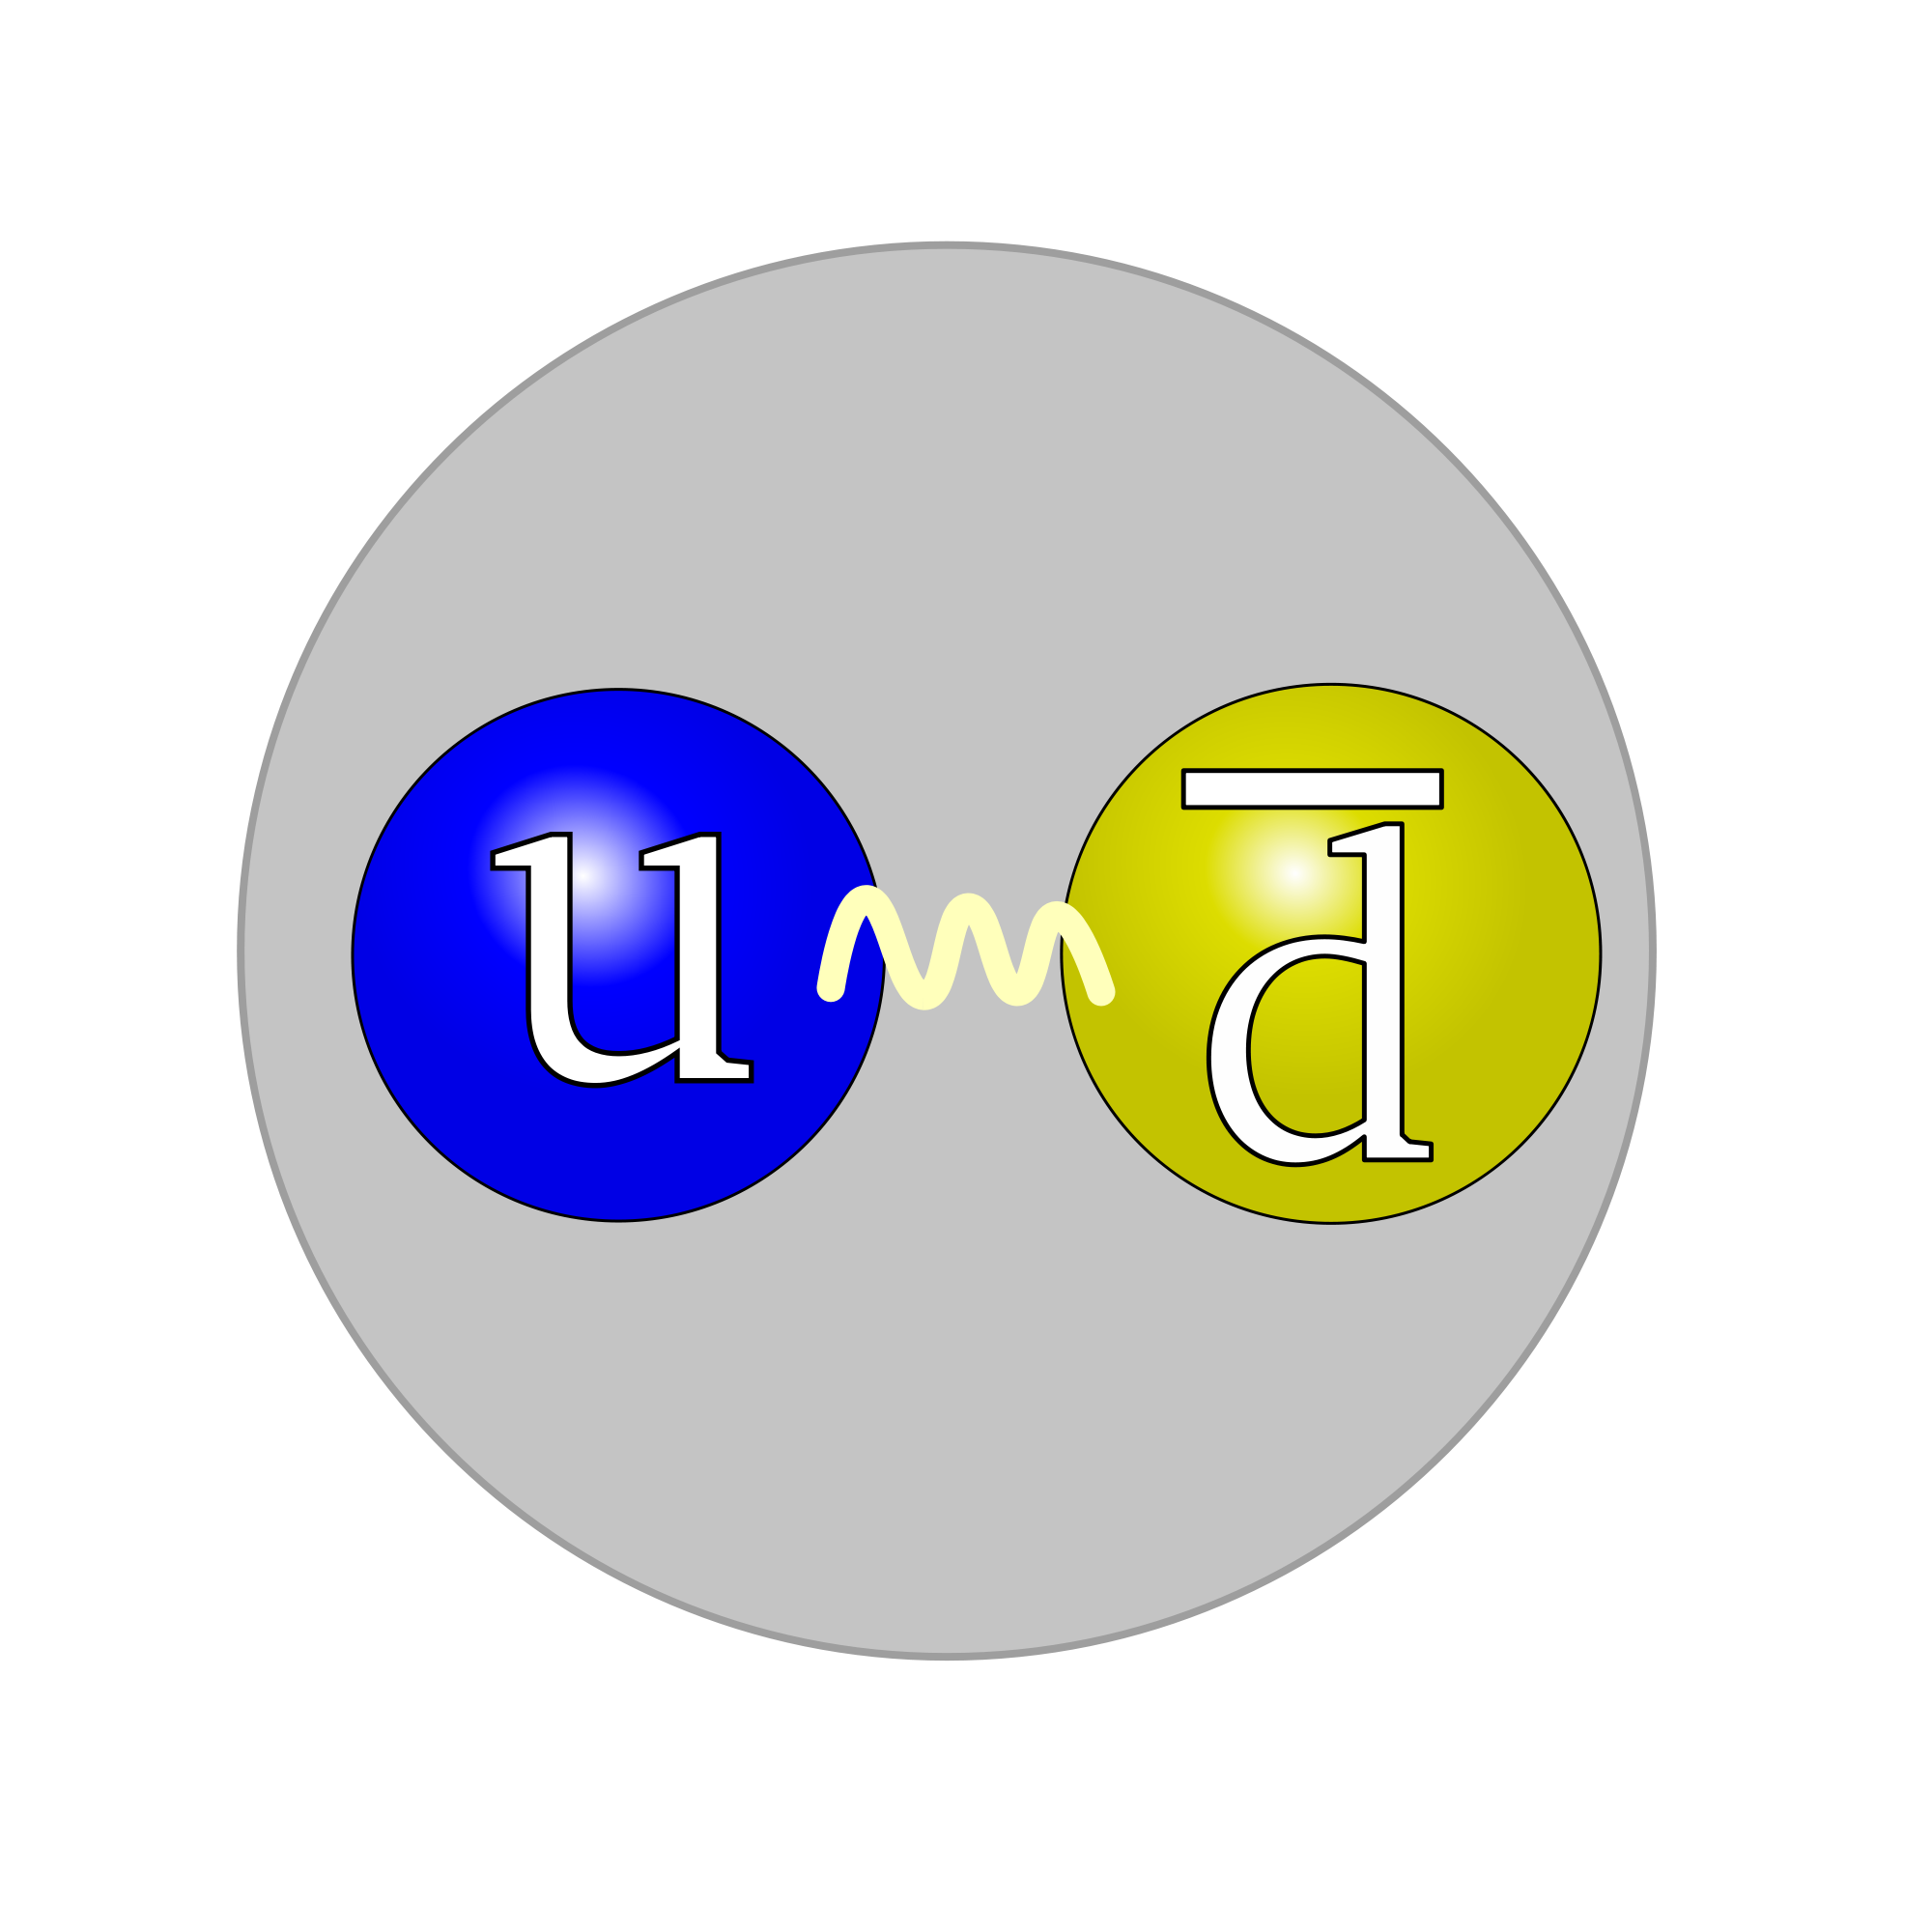
\includegraphics[width=0.5\textwidth]{ImgChap1/Meson2}
	\caption{Side view of the delta wing connector of the hodoscope}
	\label{DeltaWingSide}
\end{figure}

\begin{figure}[!ht]
	\centering
	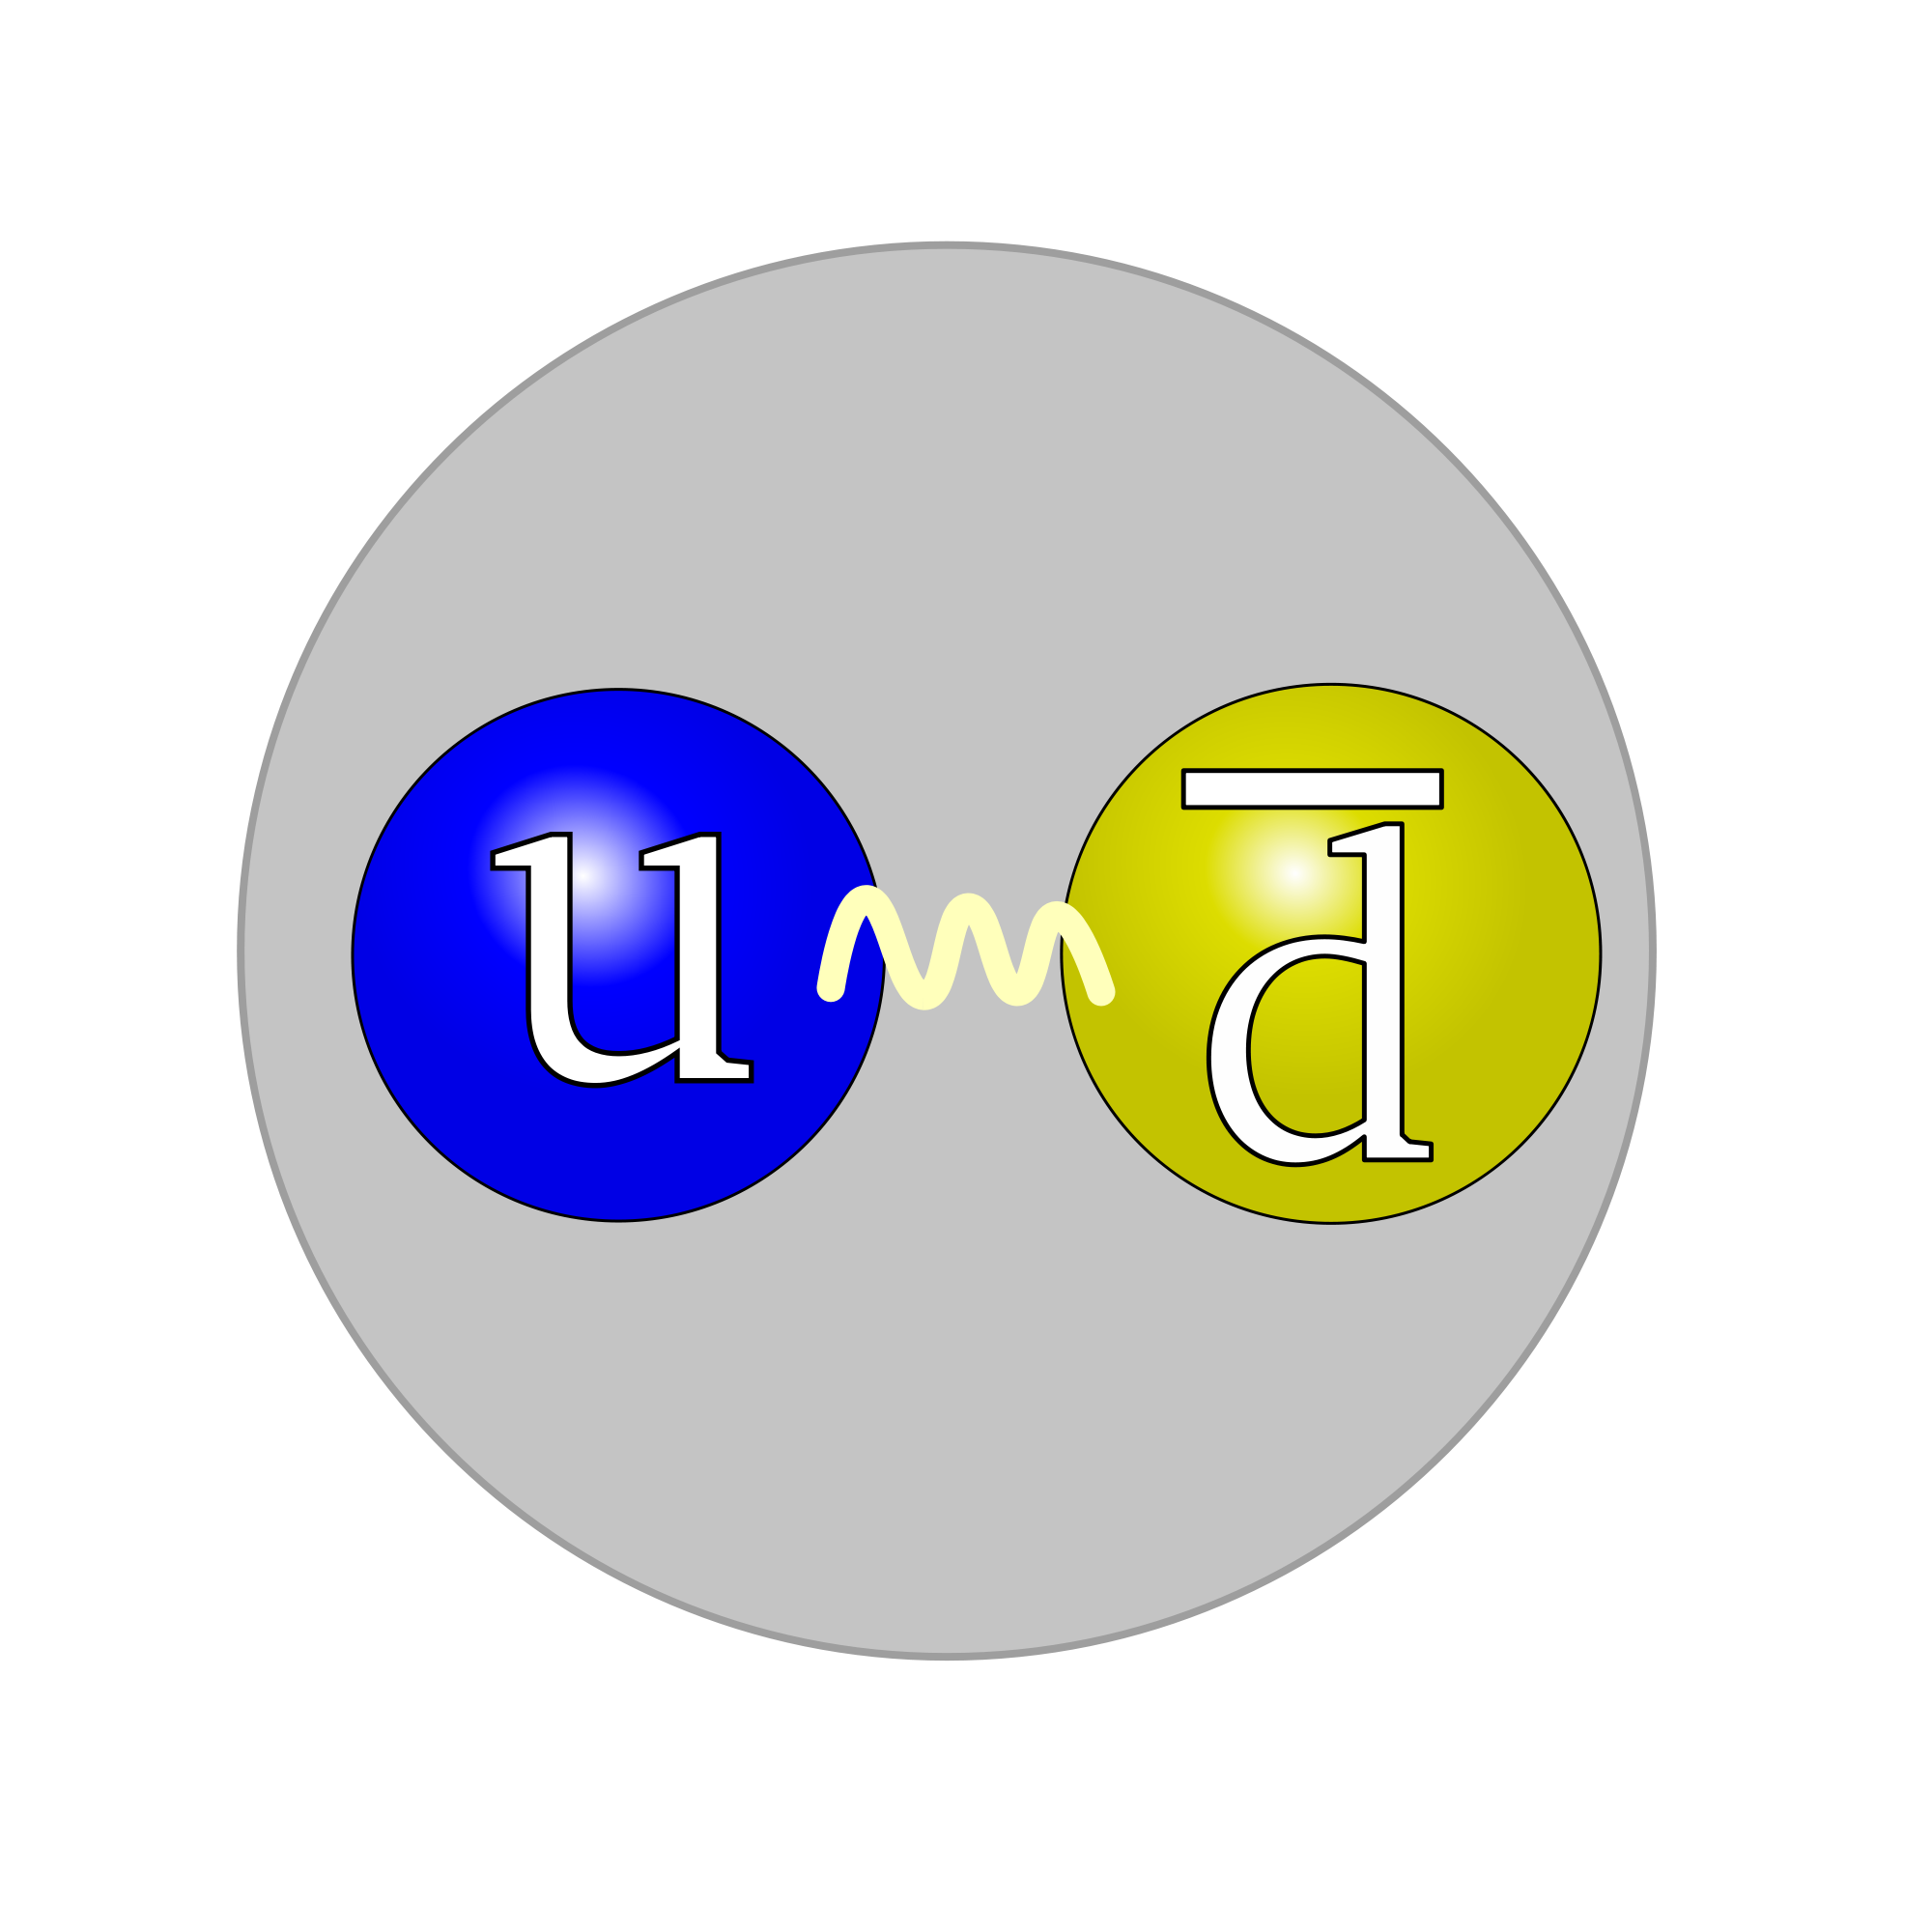
\includegraphics[width=0.5\textwidth]{ImgChap1/Meson2}
	\caption{Top down view of the delta wing connector of the hodoscope}
	\label{DeltaWingTop}
\end{figure}



\subsubsection*{Fishtale Fibre - SiPM connector}

The fishtale connections create a sealed juncture between the optical fibres and the Silicon photomultipliers. They act to guide the fibres precisely into position and maintain their optical isolation from the external environment. The connectors are 3d printed to create a consistent precise design to interface to all 30 groups of SiPMs. The fishtale connector is composed of 3 components, the main body comprising most of the length of the connector which takes in the appropriate fibres seperating from the main transport bundle of the detector. An interlocking end piece which interfaces with the electronics board and into which the fibre optic cables are glued. Finally a lipped lid which seals the construction from outside sources of noise. The fibres entry the main body through a flaired opening, which narrow to a channel just wide enough for 8 3.6mm sheaths to fit through, before curving wider, following a similar contour to a wine bottle. The flair entrance enables a wider angle of acceptance of fibre bundles. The narrow opening helps to minimise any light leaks into the component. The widening body allows the fibres to evenly spread out and be guided towards their respective SiPMs with a wide radius of curvature, minimising any loss of light and stress on the fibres. The fibre bundles pass through the main body still incased in their protective casing up until their juncture with a recess into the end piece of the connector, maintaining the isolation of fibre optics. 

\begin{figure}[!ht]
	\centering
	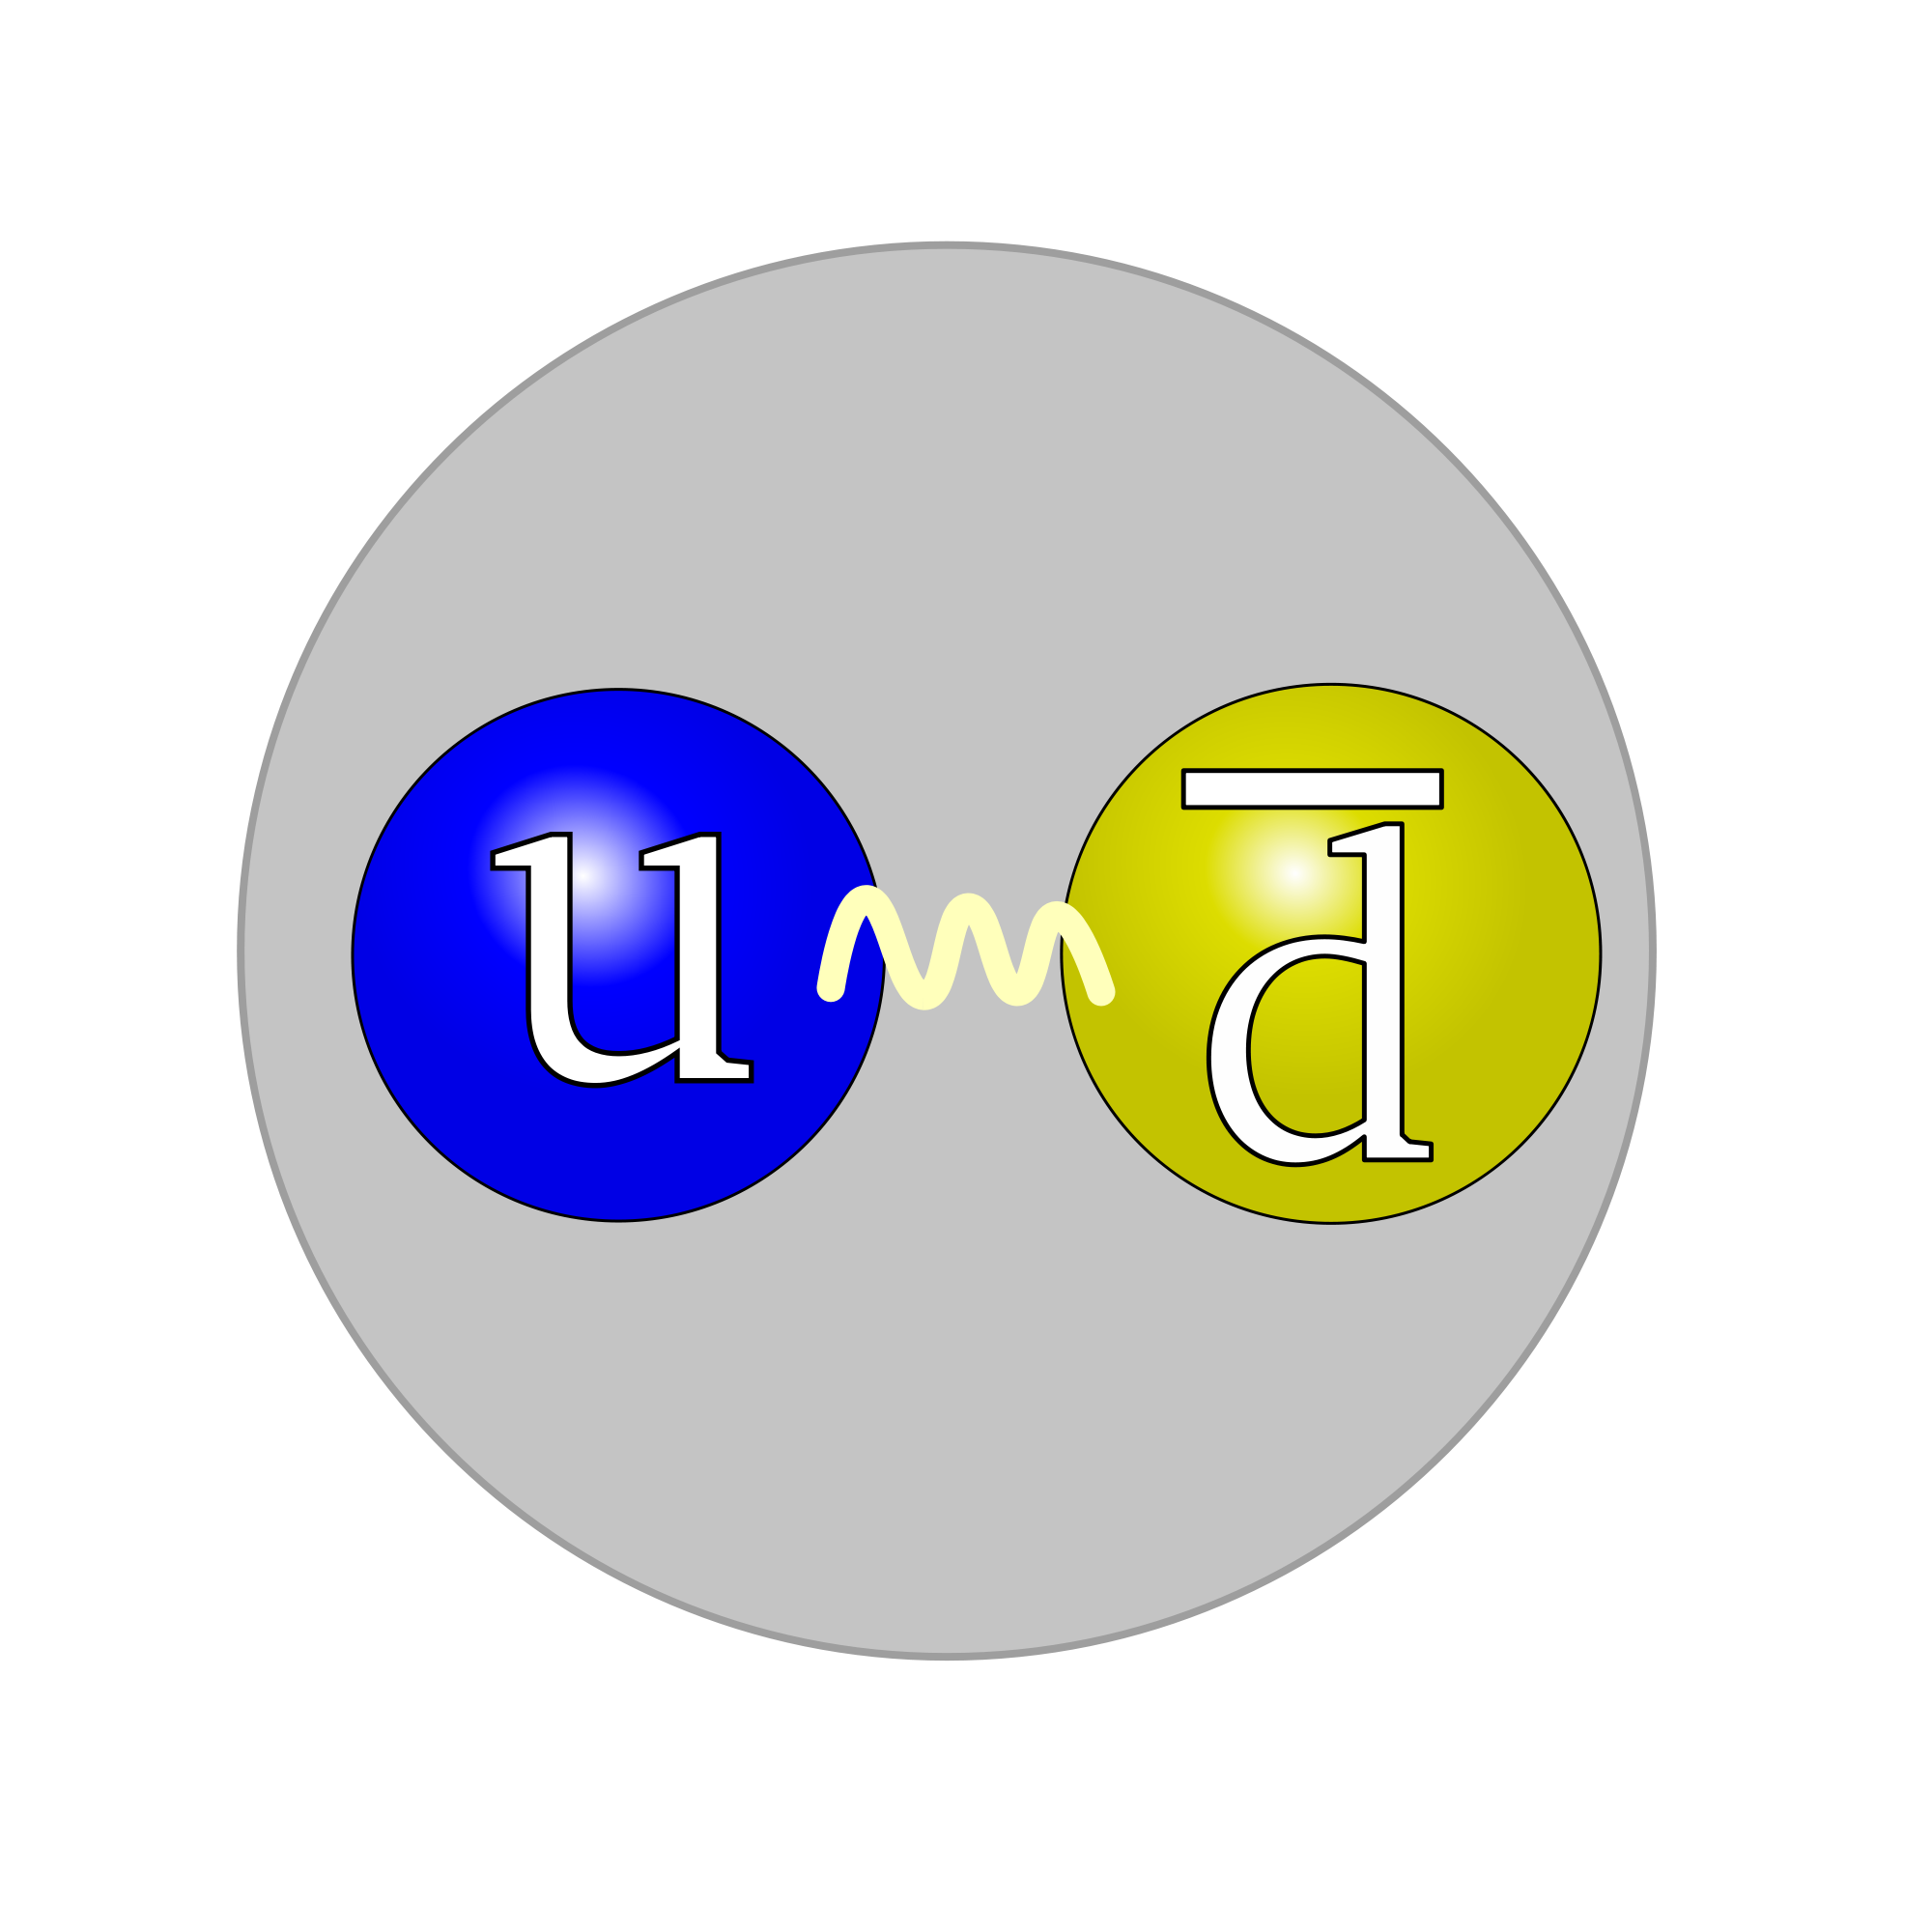
\includegraphics[width=0.5\textwidth]{ImgChap1/Meson2}
	\caption{Fishtale connector image}
	\label{FishtaleComplete}
\end{figure}

\begin{figure}[!ht]
	\centering
	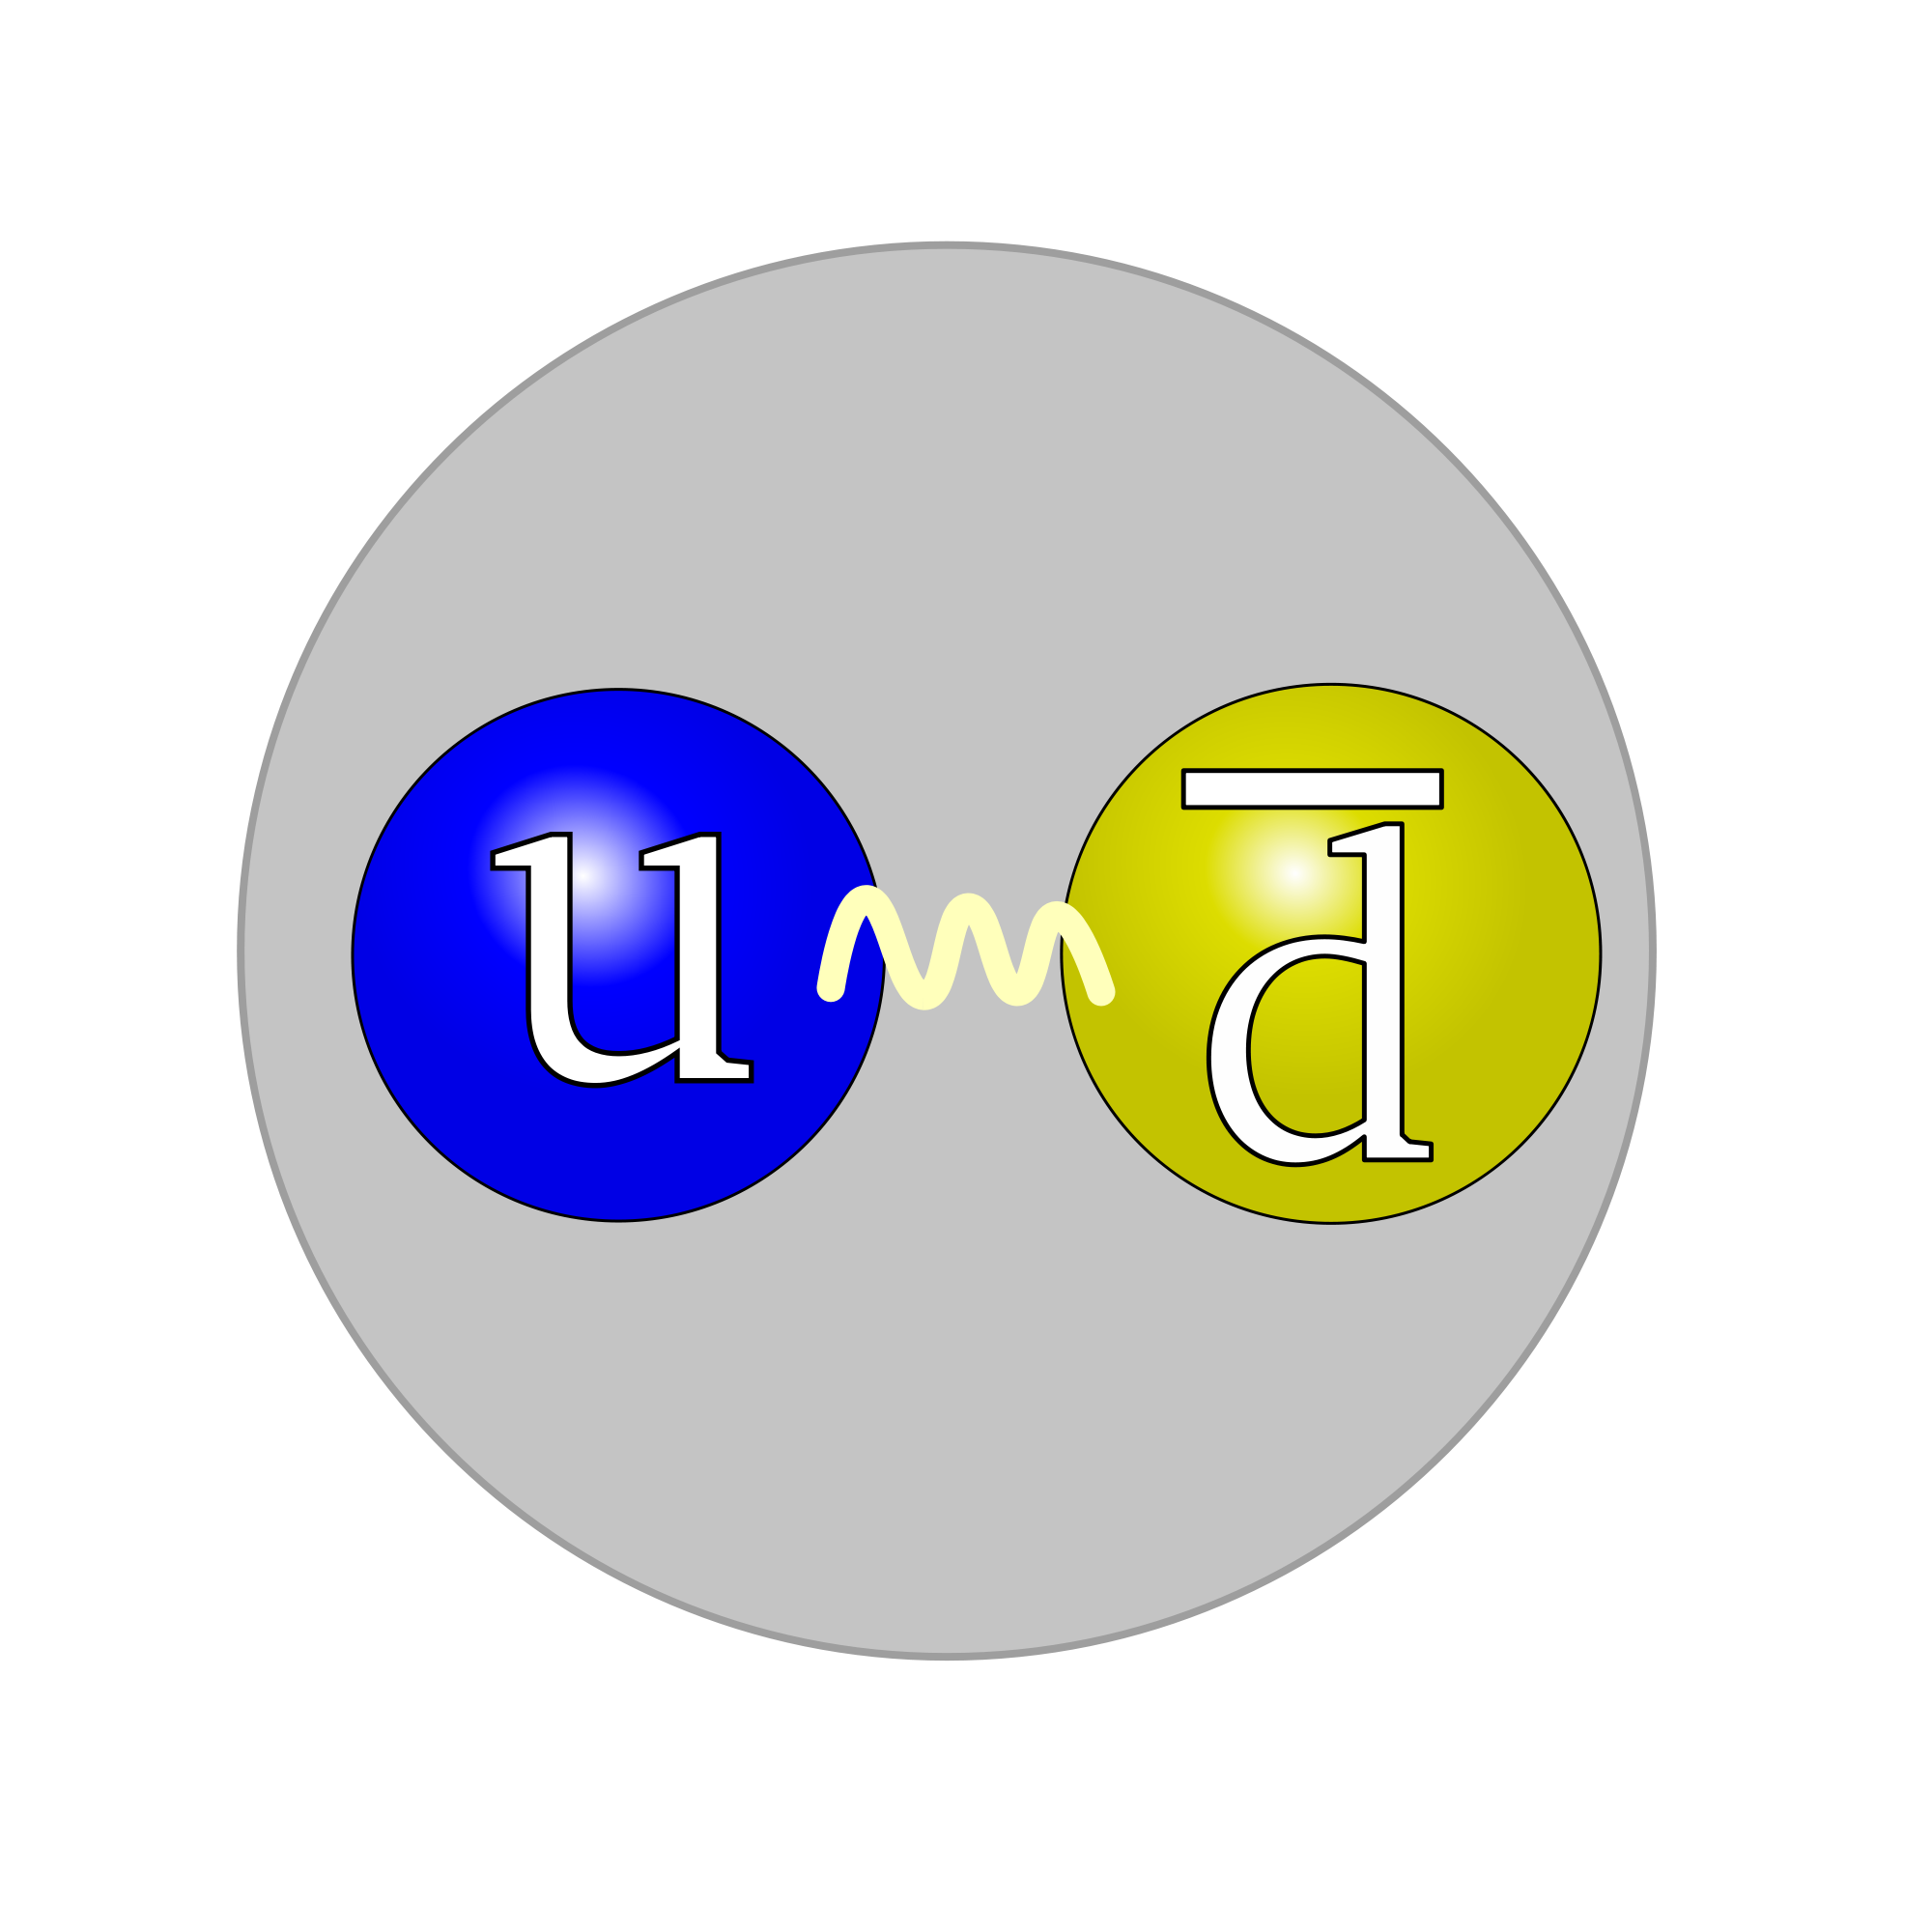
\includegraphics[width=0.5\textwidth]{ImgChap1/Meson2}
	\caption{Deconstructed fishtale connector image showing the different components of the fishtale connector}
	\label{FishtaleDeconstructed}
\end{figure}

It's critical that the optical connections formed between the connectors and the SiPMs are consistent between channels to maintain the calibration of the detector system.

\subsubsection*{Electronics Enclosure}

Carbon fibre plates
Band around the edge of the detector.
3d printed components
delta wing.
fishtail connectors
connector blocks with screws.
central ring fitting onto the tungsten pipe.
Support structure for the fibres passing through CLAS.
Electronics crate, light tight and cooled maybe.
Supastructure for construction, and transport.
etc.

\subsection{Lightsealing and protection}
How the different sections of the hodoscope are isolated from any outside sources of light and also crosstalk between elements, fibres and the electronics.


\subsection{Silicon Photomultipliers}

Silicon photomulitpliers (SiPM) are a very highly sensitive radiation detector with high efficiency and potential for very precise timing resolution. They are designed to trigger on single photons of light with high efficiency producing a signal with high gain and very low time jitter of <100ps. They are designed to be highly segmented allowing many photons to be detected simultaneously, with each element isolated from one another to avoid unnecessary background noise producing highly precise clean signals.

SiPMs consist of a matrix of highly sensitive micro cell (pixels) all connected in parallel. Each one is composed of a Geiger-Mode avalanche photon diode (GM-APD)with a connected to a resistor for passive quenching, Figure \ref{SiPMCircuit}. When operating above a certain breakdown voltage the diode rapidly discharges once triggered by a photon or another source of noise producing a signal with a high gain, before the resistor acts to quench the discharge and the cell will switch to a recovery mode where the capacitor in the diode is recharged ready to trigger again. 

\begin{figure}[!ht]
	\centering
	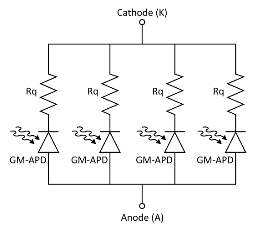
\includegraphics[width=0.5\textwidth]{ImgChap1/SiPM1}
	\caption{A schematic representation of the parallel arrangement of Geiger-Mode avalanche photo diodes with quenching resistors in a silicon photomultiplier. \cite{website:AdvanSiDSiPMpdf}}
	\label{SiPMCircuit}
\end{figure}

\begin{figure}[!ht]
	\centering
	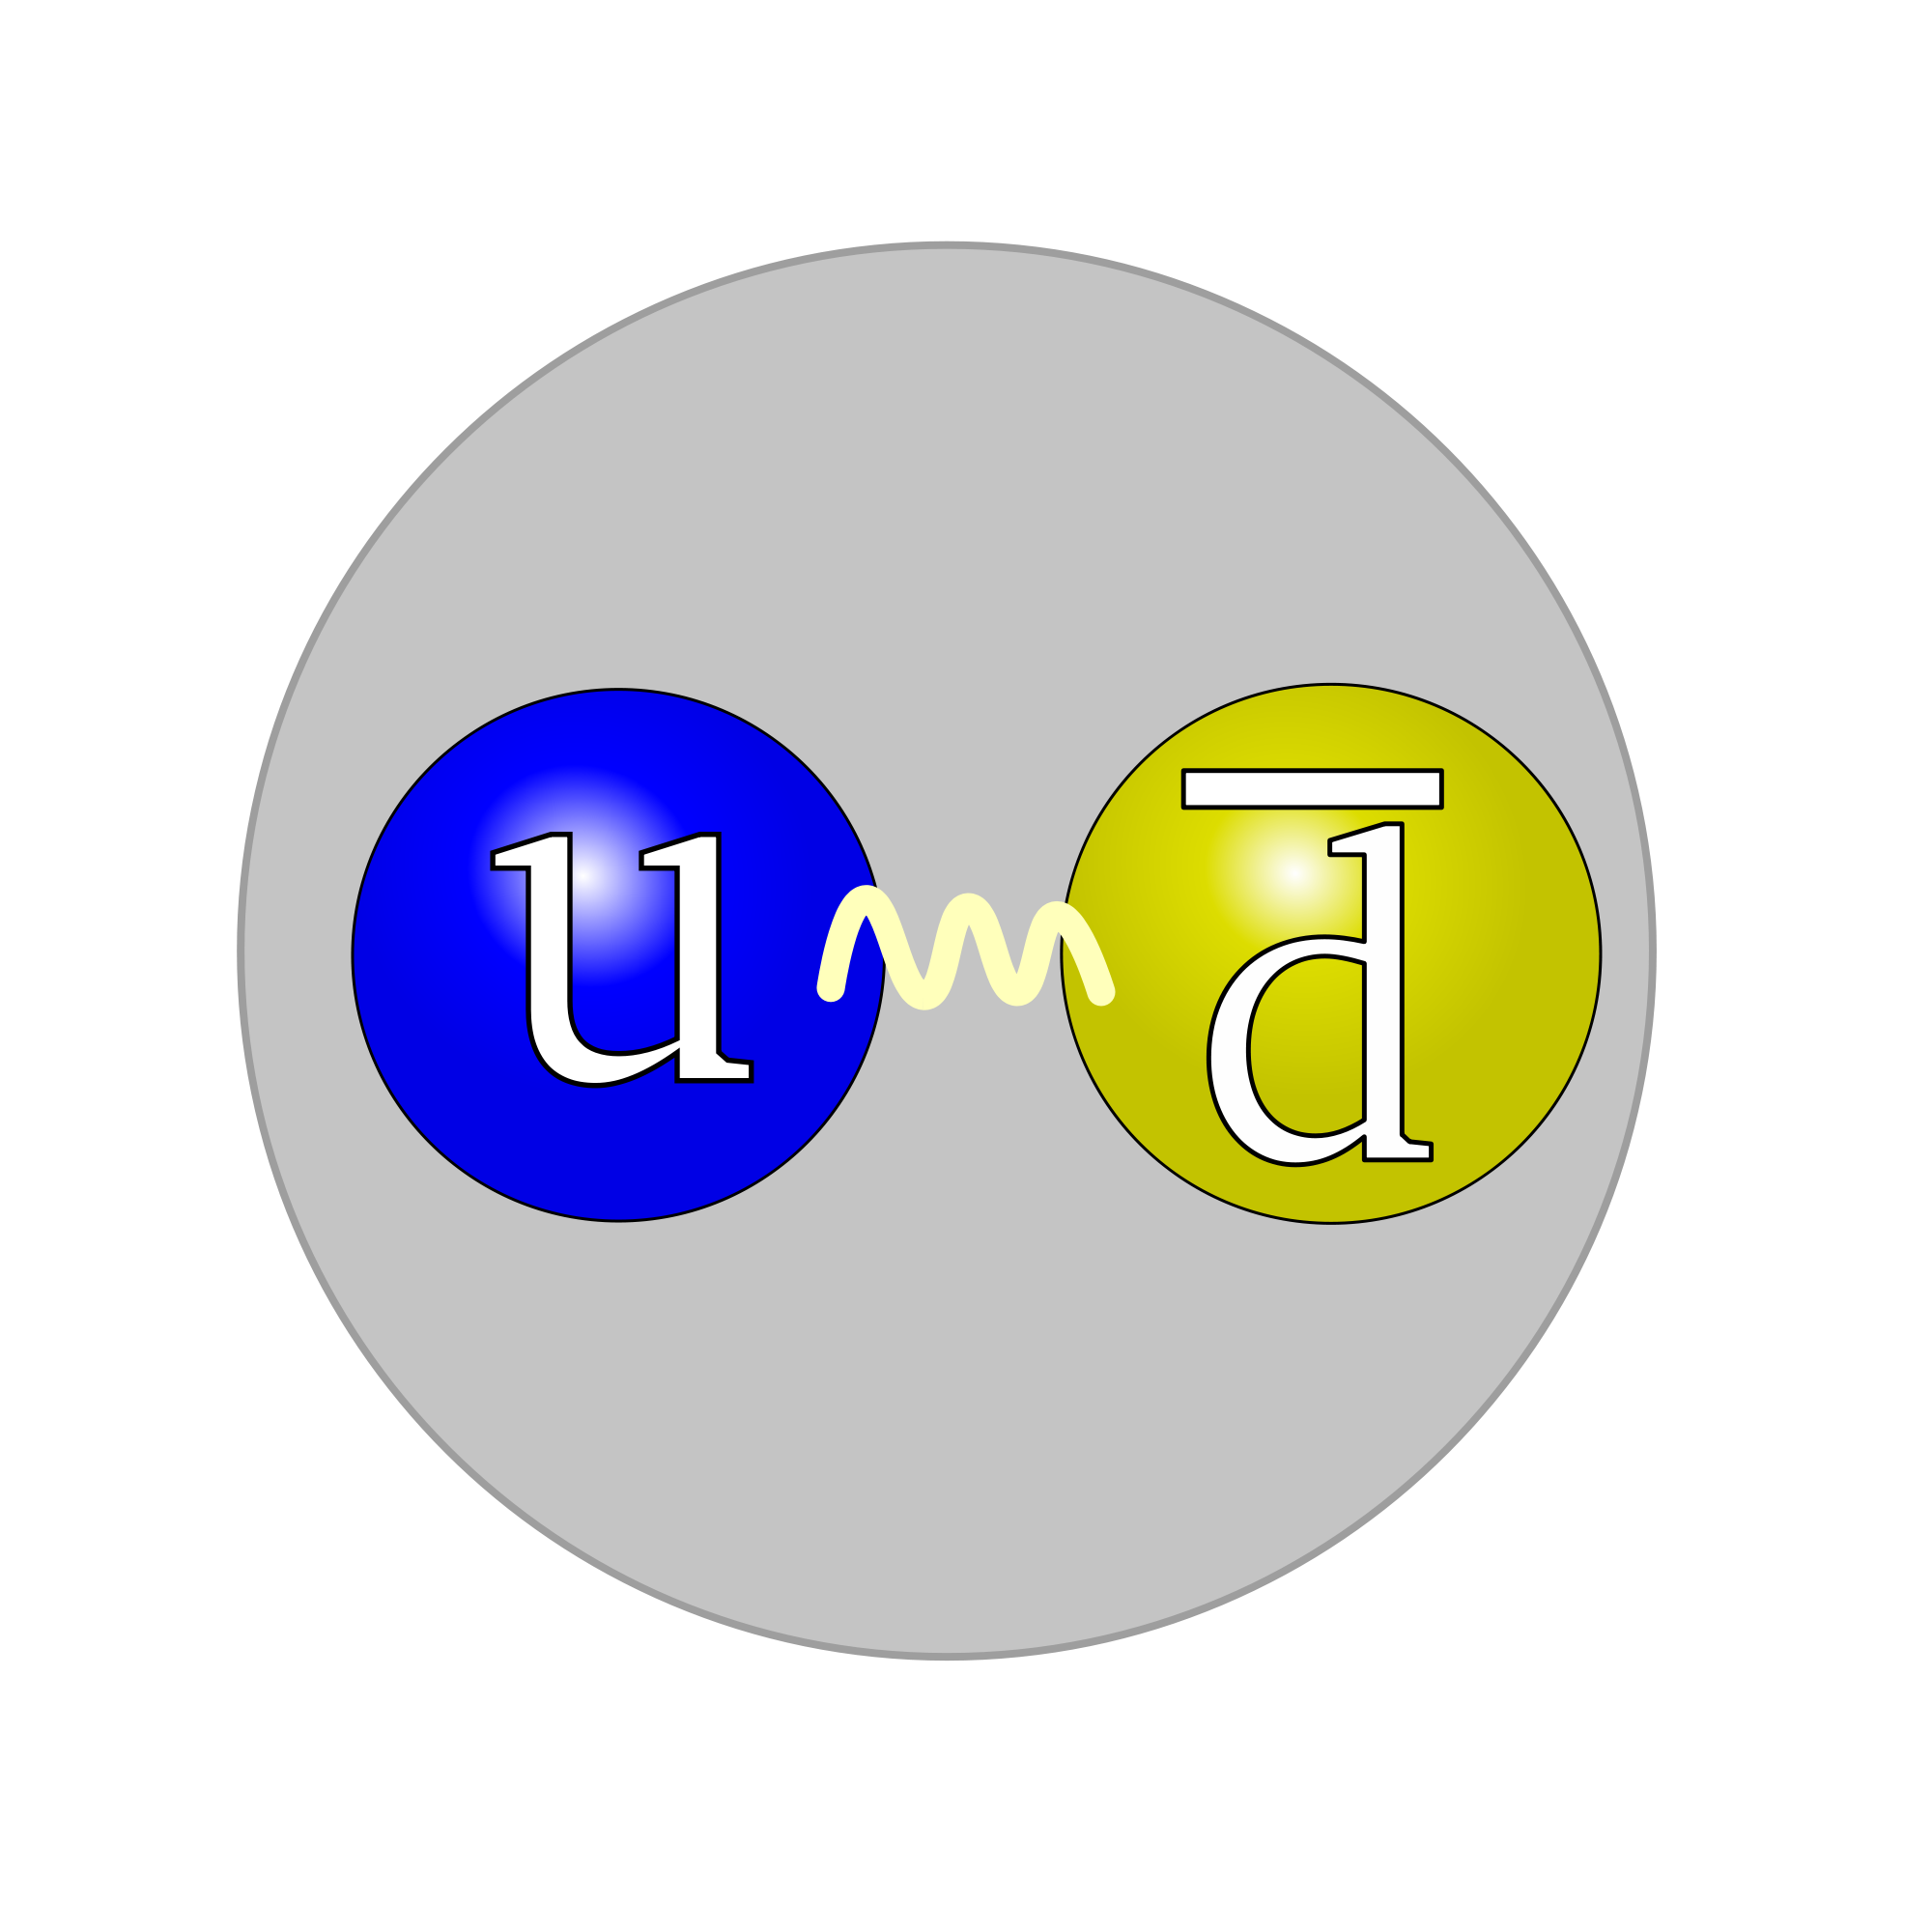
\includegraphics[width=0.5\textwidth]{ImgChap1/Meson2}
	\caption{Picture of a typical SiPM signal showing the rapid discharge phase followed by the slower recharge phase.}
	\label{SiPMDischargeRecharge}
\end{figure}

\subsubsection*{Photon Detection Efficiency}

The probability of a pixel triggering on the arrival of a incoming photon to the SiPM is known as the photon detection efficiency (PDE). This is defined as a product of three factors, quantum efficiency, triggering probability and geometry efficiency: 

\[ PDE(OV) = Qe \times Pt(OV) \times Ge \]

Quantum efficiency (Qe) expresses the probability that a photon transitions into and is absorbed by the silicon and is converted in an electron/hole pair. Qe is a function of the photons wavelength and and angle of incidence upon the SiPM. This factor is the critical reason for the wavelength shifting fibres used in the hodoscope. Triggering probability (Pt) is the likelihood that an electron/hole pair successfully triggers a sustained avalanche process resulting in a current pulse. This value is highly dependent on the overvoltage, above breakdown, applied to the circuit. Rising rapidly with increasing voltage. Pt is also wavelength dependent as the probability of generating an avalanche depends on the creation position of the electron/hole pair, which is dependent on the wavelength of the incident photon. The geometry efficiency also known as the fill factor, is a function of the amount of dead area present on the surface of the SiPM. This is a necessity to accommodate structures to isolate the pixels from one another, however with improved designs and advancing techniques for silicon lithography, the active area of the device can be optimised.

\subsubsection*{Sources of Noise}

The primary source of noise in SiPMs is the dark count rate which appear as uncorrelated pulses in the absence of light. These are a result of electron/hole pairs created by thermal excitations in the active region of a GM-APD, mimicking the appearance of a genuine single photo electron trigger pulse. The dark count rate (DCR) for a SiPM is dependent on temperature, approximately doubling every 10$^{\circ}$C. It scales directly with the area of the device and is an increasing function of the overvoltage applied to it. During operation the DCR for the hodoscope will be close to 1Mhz, however because the pulses are uncorrelated, have short rise and fall times and their amplitudes are tiny compared to a signal pulse, the dark events can be filtered with a simple discriminator at the level of 1.5 photo electrons. \cite{website:AdvanSiDSiPMpdf}

In addition to the primary noise, there are two sources of correlated noise in SiPMs. Afterpulsing (AP) and optical crosstalk (OC). Both of these types of events originate from an existing current event (Either a photon event or a dark event) and are largely dependent on the current density of the original event and the trigger probability Pt. Afterpulsing results from charge carriers trapped in silicon defects during discharge that are released later during the recharge phase of a cell. This results in a new current pulse produced on the tail of the true event, typically a few ns after the original peak. Optical crosstalk involved photons that are produced during an avalanche leaking into the active area of a neighbouring cell triggering another avalanche, known as direct OC, or is re-absorbed into an inactive region of a cell. Those in the inactive region can then diffuse back into the active region of the cell causing another pulse with a short time delay (the order of a few ns) with respect to the original signal. Both AP and OC increase more than linearly with overvoltage and quadratically with cell size, for more details see \cite{gola2012sipm}.


\subsubsection*{Operation in the hodoscope}

SiPMs high efficiency, high gain, fast timing responce and ability to trigger on single photons make them ideal for a fast timing scintillating detector such as the FT-Hodoscope. They are used in place of standard photomultiplier tubes as the detection mechanism for the photons produced in each scinillator tile. Each tile is read out by a 3x3mm array of Hamamatsu SiPMs with a pixel pitch of 75 $\mu m$ and a fill factor of 82$\%$ this provides 1600 pixels for a maximum expected signal size of 200 photons. Each tile is connected to the SiPMs by fibres, which shift the wavelength of the photons into the ideal range to maximise the quantum efficiency of the SiPMs. The gain of the detectors is very sensitive to the voltage applied, they require a supply stable to within 0.01V to maintain a consistent response level. The operating voltage for each SiPM is individually calibrated and adjusted using variable resistors assigned to each channel. 

Another consideration is the operating temperature of the SiPMs, as this affects both the dark count rate and the gain of the channels. Keeping the temperature at the lower end of the operating range keeps the dark noise to a minimum and it needs to be stable to properly calibrate the gain of the detector. At lower temperatures, that suppress the level of dark noise in the detector, higher overvoltages can be applied to the system, increasing the probability that a photon generated electron/hole pair will trigger an avalanche, increasing the photon detection efficiency of the SiPM. A typical signal from a minimum ionizing particle interacting with a detector element in the hodoscope, will result a signal with a magnitude of between 40 and 100 photoelectrons. This is far larger than the levels of signals produced through dark noise, typically 1-3 photoelectrons when crosstalk is included. As a result the signal peaks can be easily seperated from the dark noise from a simple discriminator cut at the 5-10 photoelectron level without signal loss. As a result, although desirable to maintain operation at a lower temperature, the main consideration for the hodoscope is temperature stability during operation. While in operation in hall B the detector will be maintained at a nearly constant temperature by the atmosphere control systems in the hall.

When a large number of photons arrive at the detector, several parallel cells can trigger simultaneously, the amplitude and area of the pulse generated is proportional to the number of cells that fired. This allows both the integral of the pulse and the pulse height to be used to determine the amount of photoelectrons generated in the SiPMs. A signal of around 10 photoelectrons in magnitude would be enough to have confidence that a pulse is a signal not generated through thermal excitations. However, simulations indicate that producing a signal of 40+ photoelectrons is required to produce the <500 ps timing resolution the detector is designed to surpass.





Short Paragraph about how they fundamentally work, how they recover and when they are ready for operation again. Cover breakdown voltage etc. Can talk about how this is affected by temperature here maybe?

Photon detection efficiency, what affects this etc? 

Noise sources.

How they fit into the operation of the hodoscope.

High frequency dark current.
High gain for small signal.
High signal to noise ratio when triggered.
Very sensitive to light leaks.
Very sensitive to voltage range. Requires a relatively low high voltage at around 70V. But ideally requires a HV sensitve to 0.01 V. for effective calibration.
Sensitive to temperature range.
Do not work up to a certain voltage then rise in gain quickly beyond this.
Noise peaks can be used for calibration.
Different pixel sizes. A single pixel can only fire once for each photon arriving in an event. Need enough pixels so some are not lost to double hits.
Photon conversion efficiency, Probability for a photon arriving to cause an avalanche. Function of available live area, voltage and SiPM type. Newer versions greatly improved these properties.
Output from the detector needs to be spread accross the surface of the SiPM to maximise light trigger efficiency.
3x3 arrays of sensors used for this detector system. $75\mu$m pixels. Ammount of dead area reducing with new generations.
Reduction in cross talk between pixels. Multi pixel noise mostly due to cross talk between nearby pixels causing near simulataneous firing.
Works in strong magnetic fields, not necessary in this experiment but may be of relevance in the future. Normal PMTs cannot work in that environment.
Tiny size allows them to be packed very densely allowing possibilities for extremely finely segmented detectors with individual read-out for each channel.

Fundementals, how to they work? Limited information on the electronics as this is not an area of expertise.
Focus more on their strengths and weaknesses and applications to physics.
Discuss quantum efficiency, trigger probability and fill factor combining to produce the photon detection efficiency.
Discuss gain and the factors that influence it.
Discuss noise, both primary (dark noise) and correlated (afterpulsing, crosstalk etc.)

\cite{barbosa2012silicon}
\cite{degtiarenko2011calculation}
\cite{lightfoot2008characterisation}
\cite{website:AdvanSiDSiPMpdf}

\subsection{Electronics}
Mezzanine and pre amp boards were developed and designed in Genoa with some feedback from our testing. Designed to work with the silicon photo multipliers. Levels of gain are critical to allow for the full dynamic range of signals to be captured. The extremely low levels of noise compared to the signal amplitude allow very high signal to noise ratio to be achieved with a low threshold discriminator.
Control boards. Adjusting the voltage and monitoring the temperature for each channel.
High and low voltage units, stability and precision voltage levels are critical.
Flash ADCs.

\subsection{Reflective materials}

High performance reflective materials are critical for optimising the optical properties of the detector. The material used to surround the scintillating tile elements requires the following properties:
\begin{itemize}
	\item High co-efficient of reflectivity  
	\item Consistent performance across tiles
	\item Minimal thickness
	\item Radiation Hard
\end{itemize}

These qualities are required to maximise the light collection of the wavelength shifting fibres improving the timing resolution of the detector. To provide consistent performance across individual elements and also over the lifetime of the detector. Finally to optically isolate each element ensuring there is no potential for crosstalk and minimising the affect of any light leaks into the system.

A high co-efficient of reflectivity is critical to keep photons produced through scintillation inside the detector elements and provide additional opportunities for photons that aren't quickly captured by the wavelength shifting fibres to reflect off the surfaces and be collected by the fibres. The co-efficient of reflectivity for a material is a function of the wavelength of light that it encounters. In this case the critical range is the emission spectrum of EJ-204, Figure , which ranges between 380nm and 500nm, peaking at around ~410nm. The higher the co-efficient of the material across the active range of the material, the higher than potential light yield from the tile.


\begin{figure}[!ht]
	\centering
	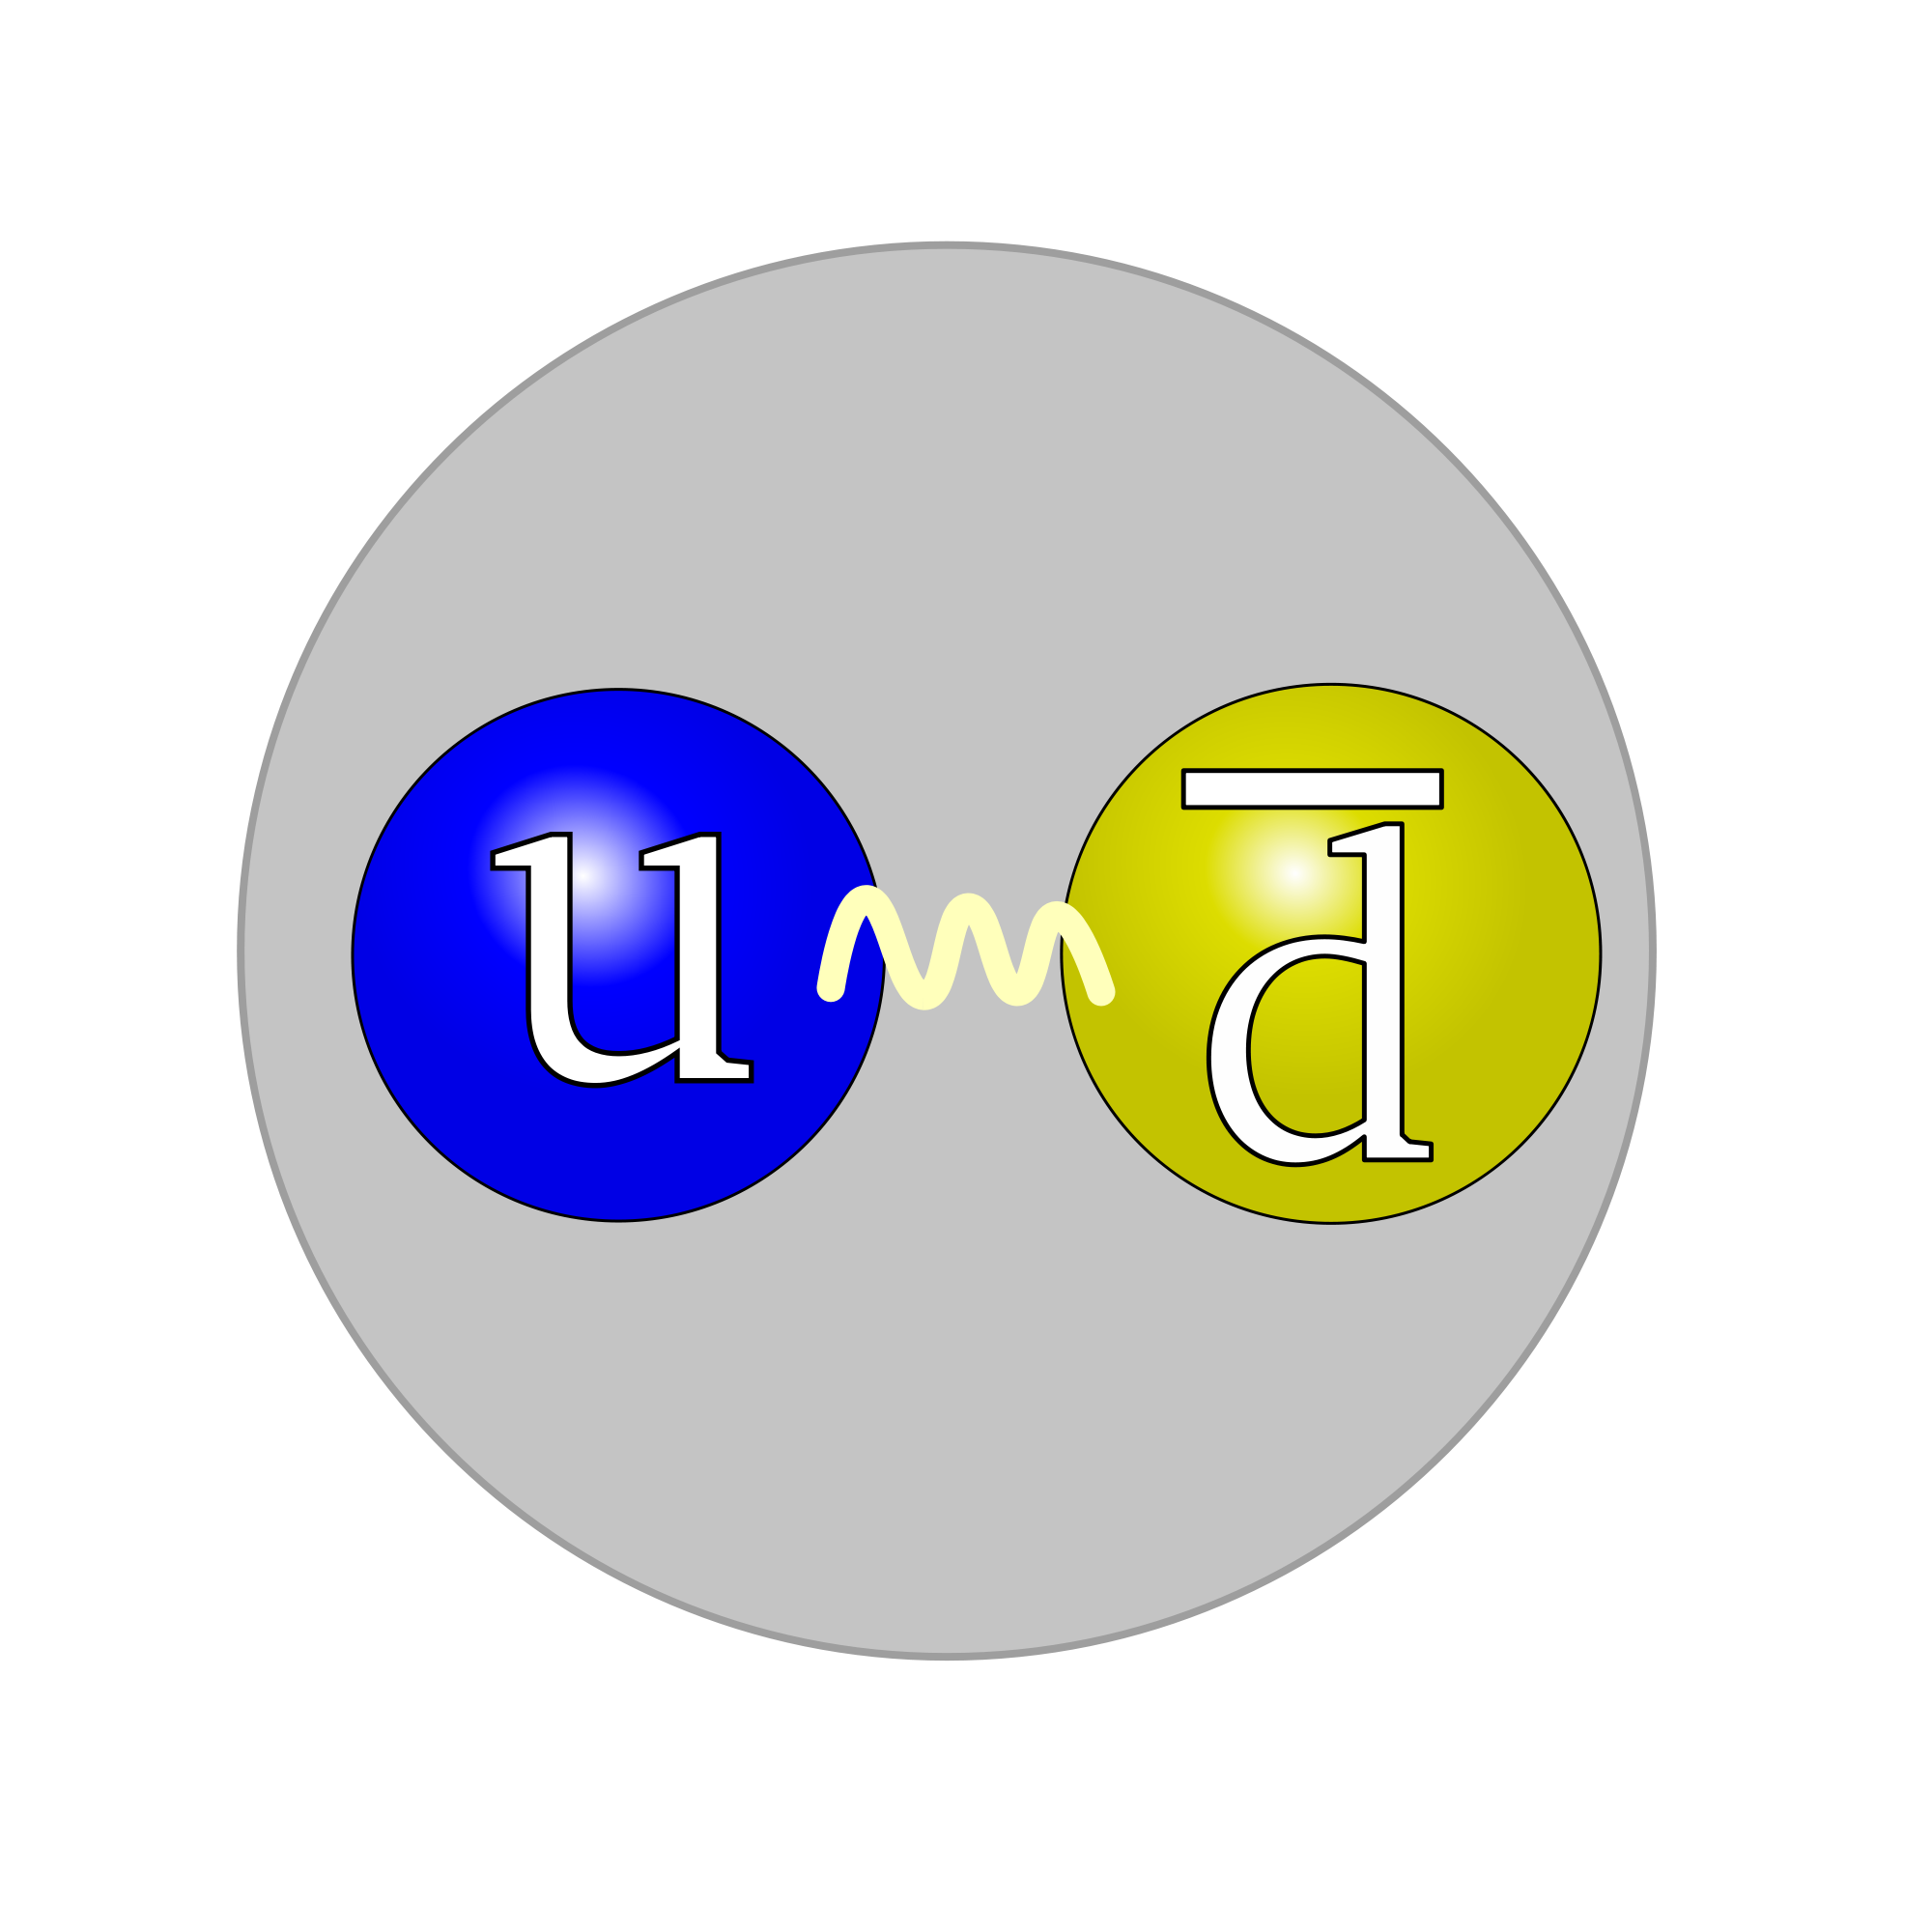
\includegraphics[width=0.5\textwidth]{ImgChap1/Meson2}
	\caption{Reflection coefficient for several reflectors as a function of wavelength.  \cite{janecek2012reflectivity}}
	\label{ReflCoef}
\end{figure}

Consistency of response to a incoming charge particle is very important in a highly segmented detector such as the hodoscope, if results from different elements are to be interpreted together. The reflective material itself must be consistent in both its response to photons but also in its juncture to the detector elements. It must be able to be moulded with precision to the shape of the detector blocks without uneven surfaces or air gaps and maintain its shape over the lifetime of the detector under the harsh radiation of the beamline. A material which may theoretically be superior in an idealised situation. May not perform or have inconsistent results when applied over many different elements. As a result systematic testing is required to ensure any materials forfill the design requirement and ease of application becomes a more significant factor than one may a priori consider.

One of the typical disadvantages of segmented detectors is a reduction in the active area of acceptance with any gaps between elements. To keep this reduction to a minimum the tiles need to be of a uniform size that will tessellate with minimal area covered by non active materials such as a reflective material. Therefore the ideal reflector is formed of a vanishingly thin layer of the material, however the reflectivity of a material is also dependent on its thickness, with multiple layers improving the co-efficient of reflectivity. In addition with minimal thickness comes fragility and often inconsistency. A balance between these factors is required.

During operation the detector and its reflective elements will be subjected to significant levels of radiation, with a typical flux of \textbf{PLACEHOLDER} krads. The reflective materials need to maintain their performance above design requirements without significant degradation over the lifetime of the detector. Replacement of the material during its lifetime will not be possible without substituting the complete detector element and possibly causing further problems with nearby elements. Only materials known to be radiation hard under these conditions were considered for use in the detector.  

Considering only materials that fulfilled the previously discussed criteria sample tiles were prepared with the reflectors shown in table \ref{ReflMatProp}. For each material tests were carried out using several samples of both p30 thin and p30 thick tiles, checking for consistency of results and any affects of the varying geometry. It also provided experience in the difficulty associated with preparing the tiles with each reflector. Considering that batch production would be required for the final system. To limit the possible variance of optical connections between the tile and the silicon photomultipliers, a simple air connection between the fibre and the tile was used which allowed the rest of the test configuration to be maintained constant for all tests. Tests were carried out using both Sr\textsuperscript{90} and Bi\textsuperscript{207} sources, both dominantly $\beta$ emitters with a range of peak energy commissions. Although data collected utilising cosmic rays would provide a more precise measure of photon output, tests conducted using sources can be completed much more quickly with statistically significant results. The trigger frequency for each tile-reflector configuration was measured for series of trigger values for a discriminator. \textbf{SEARCH OLD LAPTOP FOR FURTHER DATA ON THE RESULTS OF THESE TESTS}


	\begin{table}\centering
	\renewcommand{\arraystretch}{1.3}
	\begin{tabular}{ @{}l  c  c  c@{}} 
		\toprule
		Reflector & Reflection Coeficient & Thickness & Reference \\
		& {\small @440nm}& {\small [mm]}&  \\
		\midrule
		Titanium Dioxide Paint & 0.955 & 0.14-0.18 & \cite{janecek2012reflectivity}\\
		PTFE Tape & 0.99 & n x 0.08 &\cite{janecek2012reflectivity}\\
		Tyvek\textsuperscript{\textregistered} Paper & 0.97 & n x 0.11 & \cite{janecek2008optical} \\
		Aluminium Foil & 0.78 & 0.025 & \cite{janecek2008optical}\\
		\bottomrule
	\end{tabular}
	\caption{Properties of reflectors selected for testing}
	\label{ReflMatProp}
	\end{table}

\textbf{THE KEY RESULTS OF THE TESTS ARE SHOWN IN FIGURE}

\begin{figure}[!ht]
	\centering
	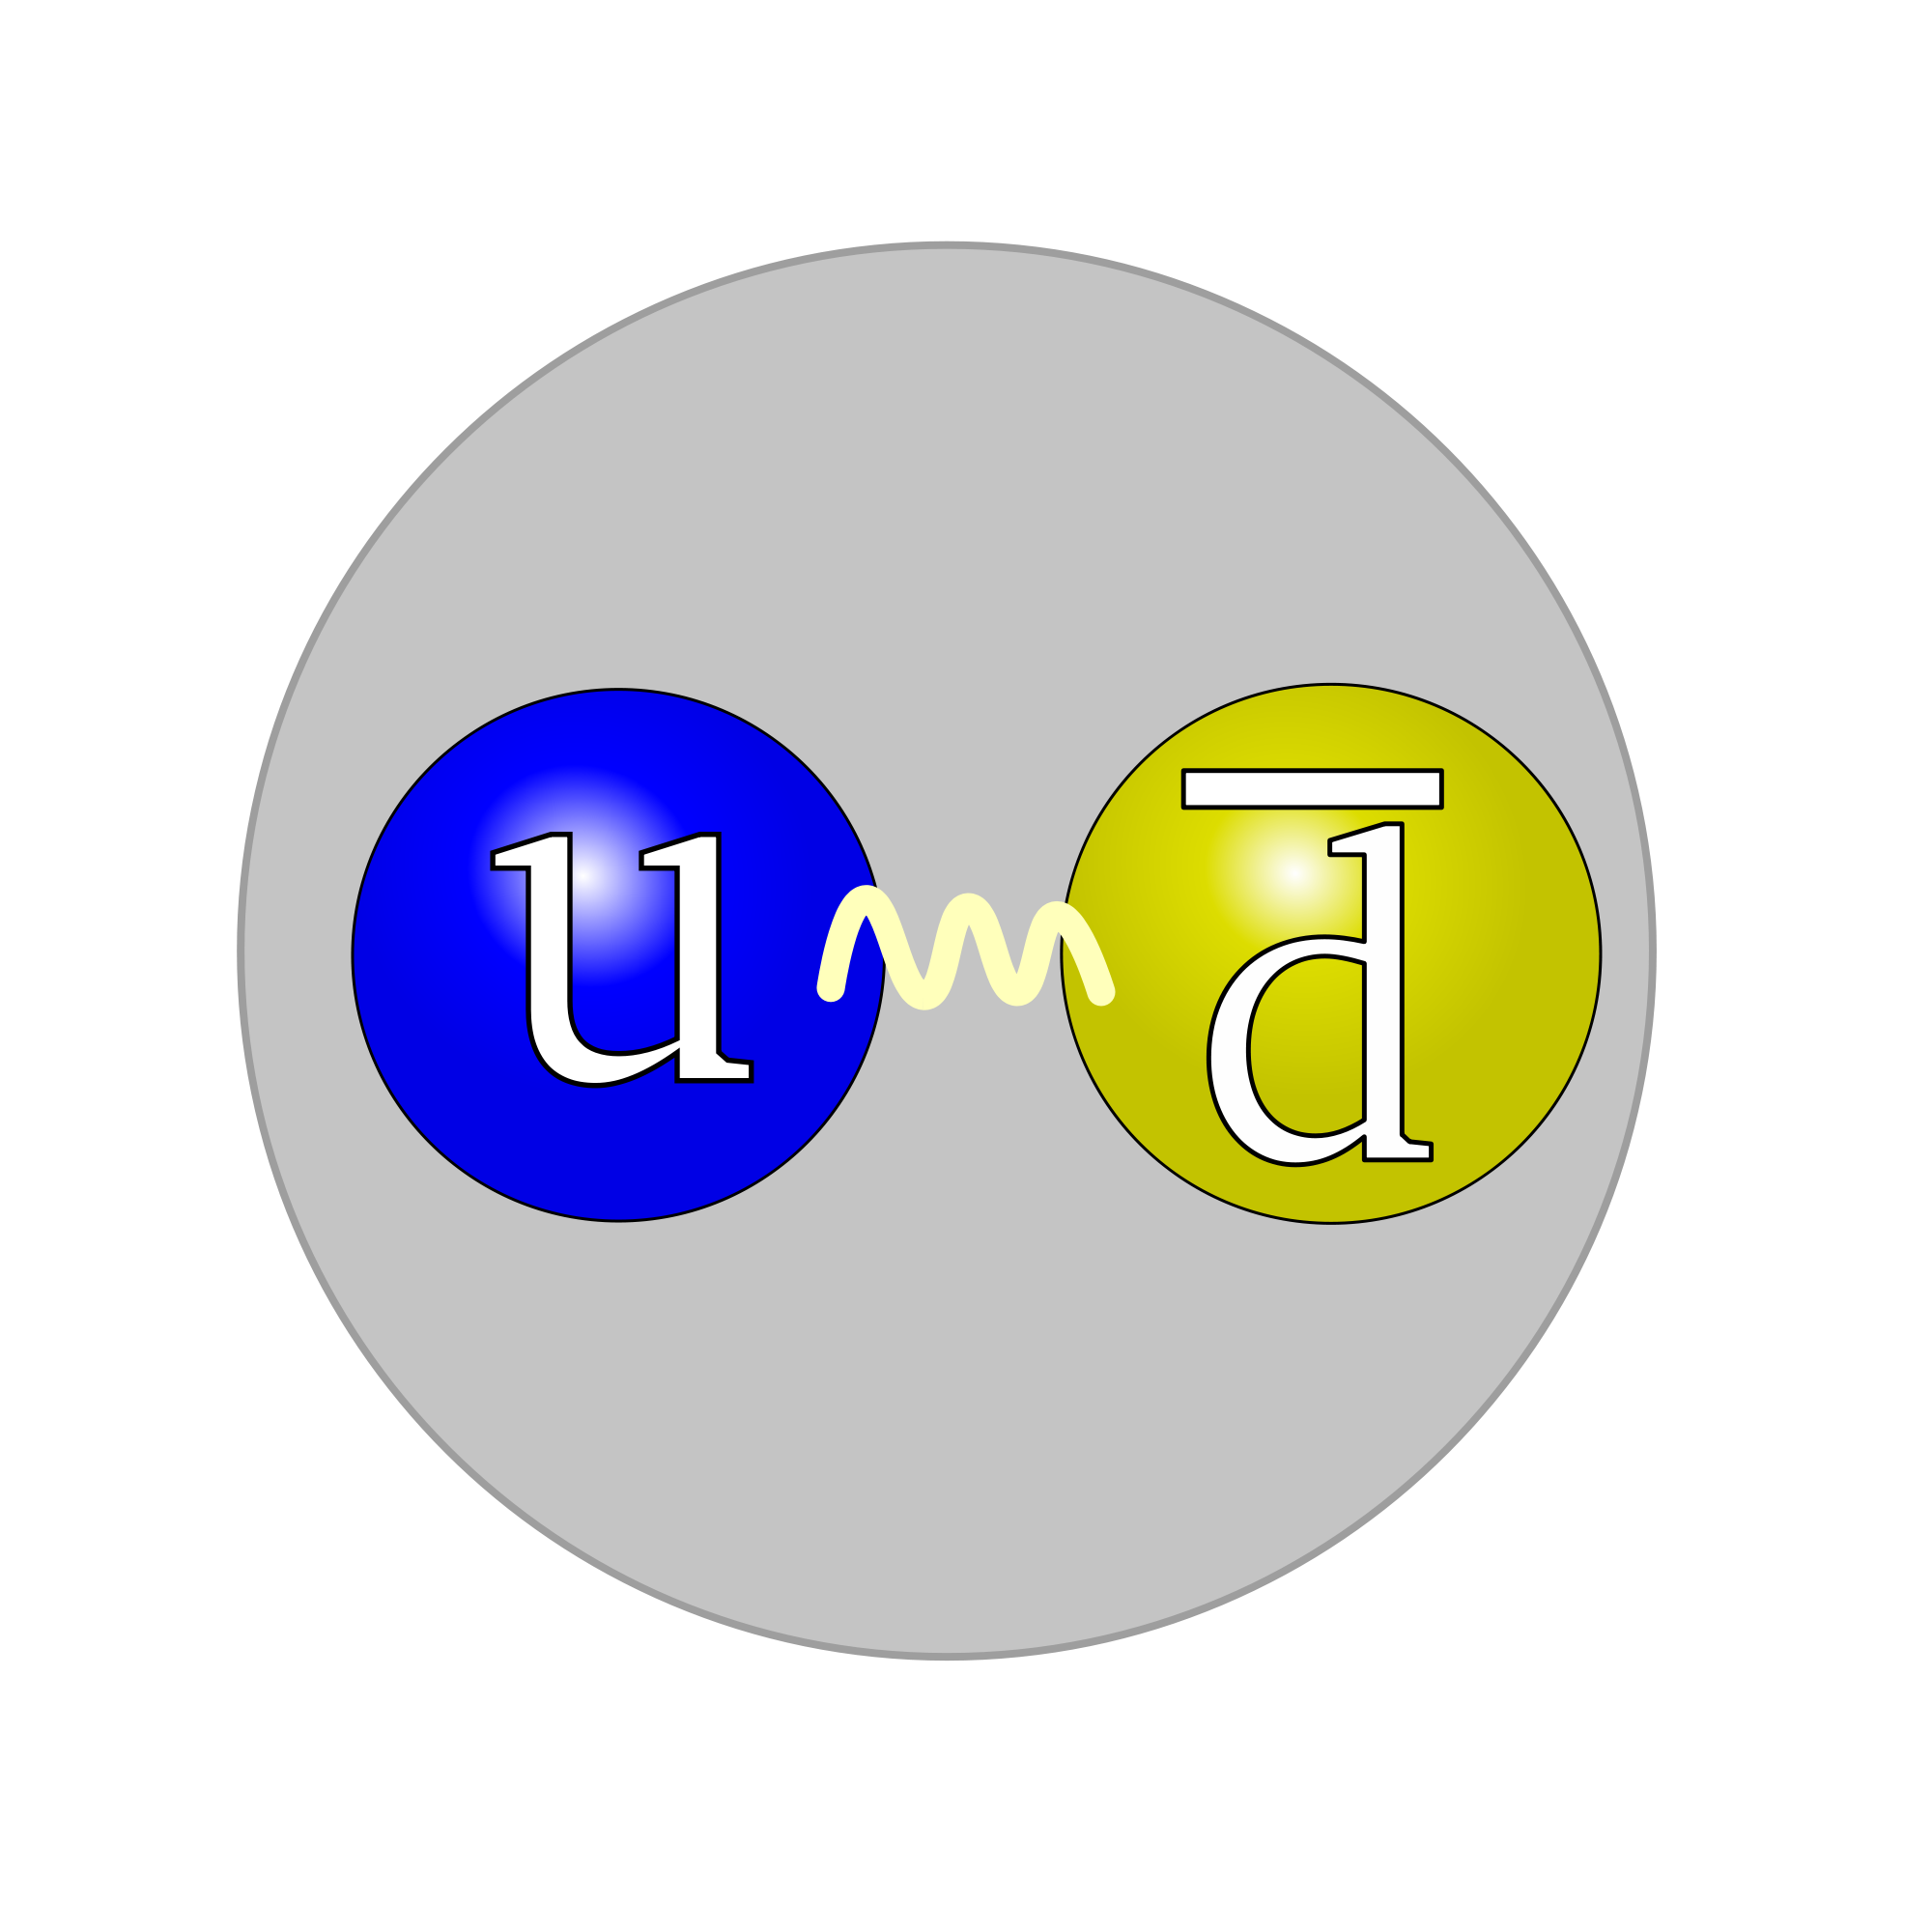
\includegraphics[width=0.5\textwidth]{ImgChap1/Meson2}
	\caption{Test results of the different reflective materials. Rate at different levels of the discriminator.}
	\label{ReflTestResults}
\end{figure}

Taking into account the literature and tests carried out the tiles. Titanium dioxide paint was selected as the material which best satisfied the demands required of the material, with a high reflective index, consistent results and ease of application. The PTFE was both thin and highly reflective, but the difficulty in wrapping the tiles with their projecting fibres in a consistent manner, was a major downside to this choice of reflector. A combination approach applying PTFE to most of the tile and covering the awkward areas with titanium dioxide paint was also considered, but discarded as the performance of PTFE was comparable to the paint in the tests carried out.

Aluminium foil was used 
Specular and diffuse reflectors.


Transition between materials important. Light loss at boundary. Change of refractive index.
Reflective paint, alumised mylar, aluminised sputtering, tyvek, ptfe etc.
Discussion of diffuse reflectors vs specular reflectors.
Issues with wrapping of the tiles.
Mirroring the ends of the fibres.
Very important to achieve consistency accross the tiles.
High reflectivity essential to achieve a large photon output after multiple reflections.
High reflectivity also essential to maintain optical isolation between elements and minimise crosstalk.
Thickness of material a major concern as this limits the acceptance of the detector. Want to be as thin as possible.
Cost also a consideration, sputtering a large number of tiles would be very expensive.
Variation of results of studies in the literature. Partly dependent on the test conditions favouring one configuration over another. Essential to carry out bespoke studies for the detector system, to ensure the right option was selected.
\cite{janecek2012reflectivity}
\cite{janecek2008optical}
\cite{weidner1981reflection}
\textbf{Need to find the other references that were used to make this decision}
\subsubsection{Mirroring of the end of the fibres}

Wavelength shifting fibres operate by absorbing a photon before remitting it in a new frequency range. For this photon to be captured and transmitted down the length of the fibre, it needs to be produced in a narrow emission of of a few degrees. The vector of re-emission is not dependent on the angle of incidence of the original photon. As a consequence, mirroring the scintillor end of the fibre, allows the angle of acceptance for capturing the photon within the fibre to potentially be almost doubled. This comes at the cost of blocking any photons that may have entered the fibre through the end of the fibre, but in a fibre of any significant length the benefits outweigh the downsides.

The ideal reflector for this purpose shares many of the same characteristics as for the scintillators, but it also has the conform to the limitations of attaching to the end of a fibre at the end of a narrow channel.  To be effective the reflector needs to cover the full area of the fibre, particularly as the multi-layered design of the fibres results in the majority of light being transported in a narrow region near the edge of the fibre. However if it is fractionally larger than the fibre it will either not fit, damage or be damaged when placed into the channel. In most examples in the literature such as the study done by Joram \cite{joram2014mirroring}. The mirrored fibres were placed in flat channels which pass all the way across the scintillator where there was easy access to the ends of the fibres. However the design of the hodoscope restricts this access and tests using an idealise reflector such as thin disks of aluminised mylar were inconsistent in tests. After these the titanium dioxide paint used as the reflector on the scintillators was considered along with aluminium sputter depsoition, which would deposit a thin layer of aluminium directly onto the fibres. However the latter option was ruled out on cost effectiveness after tests using the reflective paint proved highly effective and consistent. 

\cite{joram2014mirroring}
\subsection{Optical Connections and transport}

Transitions between transport materials are a critical element of efficient photon transport. A simplistic overview of each photons journey in a channel would start with production in the scintillating tiles, transport through the optical fibres before arrival at the the SiPMs. However there are transition points between the tile and WLS fibres, WLS fibres and clear fibres, and from the clear fibres to the SiPMs. Along with the less obvious transitions between layers in the fibres.  

Transparent materials with similar refractive indices minimise the amount of photons lost at the boundary between materials. How much of this is due to internal reflections? Consider transition radiation at boundaries, cherenkov radiation and any other effects that may contribute to the loss in signal strength.

Discussion on ideal optical properties, however these must maintain their quality under radiation and age. Affects of any annealing. Consistent properties essential for proper calibration of the equipment over time.

Possible discussion on fusion splicing could go here instead of in the optical transport section. Or could combine the two together.

Optical glues and their properties. Transmission ideal, similar refractive index, hermetic and uniform response. Radiation hard. Tested under similar conditions. Will not damage the fragile materials around it.

Comparison to an air connection, why use glue if an air connection would do? Not possible in this case due to the tension in the fibres and orientation of the hodoscope. The fibres would simply fall out of the holes! Ensuring the fibres fill the entire length of the channel, extremely important to maximise the light output of the tiles and also maintain uniform response of all the channels.

Air connection used for the SiPMs but the fibres are fixed into the connectors. Gluing the fibres to the SiPMs would make mainanence impossible. 

Glues, fibre joins, fusion spicing, fibre to SiPM.
\subsection{Glues}
\cite{kobayashi1991transmittance}
\cite{kirn1999absorption}
\cite{clements2006selection}
\cite{montecchi2001study}
\cite{cohen2003optical}
\cite{cohen2001optical}
\cite{va2014optical}

\subsection{Forward Tagger Flasher Flasher}

Used for measuring the change sensitivity of the fibres and tiles over time, by using a driver of constant manitude to radiate the system and measure the level of output throughout the lifetime of the detector.

\section{Effect of radiation on different components}
Critically the effect on the scintillator tiles and the light transport components along with the SiPM. Mostly just the components that are part of the lollypop will be under significant levls of radiation.
Discuss the annealing process for the scintillator and fibres. How this offsets the damage that the radiation will do.
The detector is shielded from much of the intense radiation by the moeller cone. 

\cite{bross1990radiation}
\cite{barsuk2000radiation}
\cite{protopopov1993radiation}
\section{Testing}
While designing each element of the detector.
Sample testing on arrival.
During construction.
Beam tests.
Photon Output.
Bend radius.
Calibration using different ratioactive sources, or cosmic rays. Problems and benefits of each method of testing.
Ideally testing the equipment with a beam similar in nature to the processes that will be carried out at JLAB. However there is limited availability of beam time and compromises are needed between rate and precision. Source vs cosmic normally.
Construction stress tests.
\section{Beamtime}
Frascati tests.
\section{Contruction}
Everything tested and built in a very low UV enviroment to protect the fibres and tiles.
Air was filtered.
Air was cooled to keep and standard temperature for testing.
Lab coats, gloves etc.


\subsection{Component arrangement and Numbering systems}
How the tiles were arranged.
Measuring the sizes of each tile to optimise the arrangement through the detector and minimise any gaps, maximising the effective coverage and this acceptance of the detector system. Focusing on the areas of highest flux where detector acceptance is most critical to be near perfect.
Arranging the position and orientation of the tiles to maximise the efficiency of the fibre packing to minimise the vertical space taken up by the fibres and reducing and pressure load on the fibres. Identifying any critical areas of strain and how to deal with these pressure points.
Arranging the fibres to fit into bundles, then how they would path through the detector, fit into the delta wing and transition through CLAS to reach the electronics.
Arranging the bundles on the way to the electronics. The bundles must fit through tight space requirements, where maximising packing efficiency is critical. The fibres must be kept protected from damage and sealed from any outside sources of light or crosstalk.
\subsection{Numbering system for the elements of the detector system}
Sections of the detector.
Fibre bundles.
\subsection{Gluing} 
Different types of glue. Studies on their transmitivity properties, effect of radiation damage, pot life (too fast and too much heat that will damage the fibres and tiles).
Precise scales and pippetes used to ensure quality and consistency of the mix. Mixed thoroughly and then put under vacuum to remove any air bubbles.
Different glues used for holding the fibres in place in the delta wings and affixing the fibres into the tiles.
\section{Detector Longevity}
Expected effect of running on the detector.
Radiation damage.
Electronic issues.

\section{Commissioning}
Calibrating, optimising, fixing any problems and resolving any unforeseen issues.
\section{Future development}
Upgrades to the electronics crate to provide fan cooling to the SiPM boards. Allowing them to be running at a higher operating voltage 
\chapter{Introduction}
A fast timing hodoscope has been developed as part of the new forward tagger to be installed as part of the 12 GeV upgrade to the Continuous Electron Beam Facility at the Thomas Jefferson National Laboratory.

Introductory section needs to illicite the key physics objectives of the program. Why these are significant and why this is the approach to determine more information about them.

Probably an introductory section focused on quantum chromo dynamics, the standard model and mesons. Providing a background for the purpose of the hodoscope and the analysis.
\section{Theory}
Probably a good idea to have a general chapter on quantum chromo dynamics, its importance and direction of research.

Quark model and its limitations. What it describes well but also what it doesn't account for. Expectations from current theory predict states beyond the simple bound states of meson and baryon.

Confinement
Complexity of the coupling constant in comparison to QED.

Why study mesons? Meson spectroscopy.

Meson Nonets produced by the possible quantum states.
Higher energy states of mesons.
Hybrid mesons, tetraquarks, pentaquarks, hexaquarks/dibarions, excited gluon couple to a meson. These states are predicted but not currently confirmed. Short lived states that allow states with normally forbidden combinations of quantum numbers.

Discussion on the observation of resonances and their place on riemann sheets in the complex plane. Resonances occuring at points of discontinuity when the function rises to infinity. Since my knowledge is limited about this area probably a brief overview would be enough.

Much of the progress in the theory in the area stalled in the 1970s limited by the experimental data available at the time. Technology has advanced in the intervening period. With new detector systems coming online, significant potential for breakthroughs in the area. Lattice QCD also providing a new avenue for progress with the growth in computation power available in parralelised cpu farms. These developments provide constraints to the theory and helping to guide the experimental search. 


Experimental facilities researching hadronic nuclear physics. Compass, JLAB, MAINZ, BES-III, CERN, SLAC etc. 

Theory and background papers
\cite{dudek2011lattice}
\cite{jaffe1977multiquark}
\cite{bali1993comprehensive}
\cite{johnson1975bag}
\cite{dombey1969scattering}
\cite{schilling1973analyse}
\chapter{Jefferson Lab and CLAS}

\section{Background}
The Thomas Jefferson National Accelerator facility, more commonly known as Jefferson Lab or JLab, is a U.S. national laboratory located in Newport News, Virginia, U.S. Its physics program is designed to probe the structure of hadrons to better understand the fundamental properties of nuclear matter. 

\begin{figure}
	\centering
	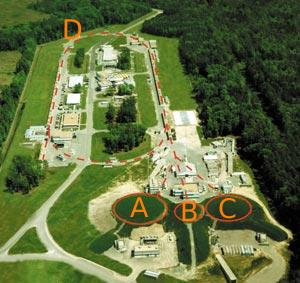
\includegraphics[width=0.6\textwidth]{ImgChap1/jlab1}
	\caption{Photograph of JLAB}
	\label{JLABAirial}
\end{figure}

The research program at the laboratory is based around the Continuous Electron Beam Facility (CEBAF) a superconducting radiofrequency based accelerator based around two anti-parallel linacs linked by 9 recirculation beam lines that allow up to 5 passes through the system. The facility produces a continuous wave electron beam with energies exceeding 6 GeV and luminosities of $< 10^{38} cm^{-2}s^{-1}$. For further information on CEBAF see \cite{leemann2001continuous}.

\textbf{Some further detail on the beamline.}

\begin{figure}
\centering
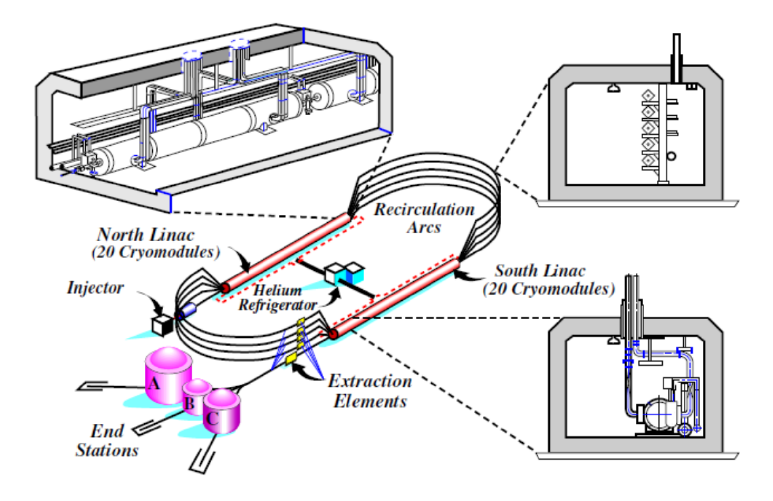
\includegraphics[width=0.6\textwidth]{ImgChap1/CEBAF1}
\caption{A schematic layout of CEBAF.}
\label{CEBAF}
\end{figure}

The primary beam is separable and the facility is capable of delivering beams to 3 different experimental halls for simultaneous experiments. Each of the experimental halls in CLAS is designed to be complimentary providing different facilities address a broad range of physics goals.

\begin{figure}
	\centering
	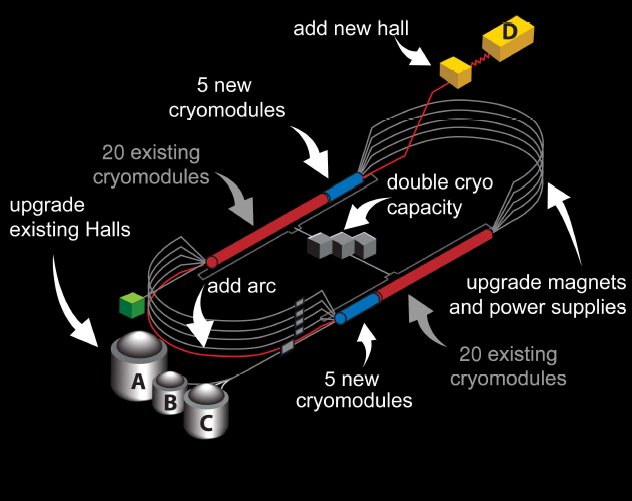
\includegraphics[width=0.6\textwidth]{ImgChap1/CEBAF}
	\caption{A schematic layout of CEBAF after the 12 GeV upgrade is completed.}
	\label{CEBAF12}
\end{figure}

In June 2010 construction began on an $\$338$ million upgrade to Jefferson Lab upgrading the beamline to a maximum energy of 12 GeV and adding a fourth experimental hall to the facility (Hall D). The investment also includes upgrades for the existing experiments in halls A, B and C. Presenting both new challenges and opportunities for the working groups. 

Hall A is equipped with a pair of identical high resolution spectrometers capable to processing luminosities $< 10^{38} cm^{-2}s^{-1}$. Its research program includes work on nucleon structure functions and nucleon form factors. \cite{alcorn2004basic}

Hall B houses the CEBAF Large Acceptance Spectrometer a wide acceptance detector designed to study electro and photo induced nuclear and hadronic reactions. The detector required efficient detection of both charged and neutral reactions products to be able to study exclusive reactions. \cite{mecking2003cebaf}

Hall C main focus is a pair of \textbf{Missing Detail for Hall C}

Hall D \cite{qiang2015detector}


The work presented in this thesis is focussed around physics undertaken in Hall B at JLab and the CLAS detector situated within it.

\section{CLAS}
CLAS is a wide acceptance detector utilising a toroidal magnetic field that is situated in Hall B at JLab. Its primary design aims are to measure the momentum of charged particles with high resolution, covering a wide geometric area up to large angles in the laboratory and keep a magnetic field free region around the target, to allow the use of dynamically polarised targets.

\begin{figure}
	\centering
	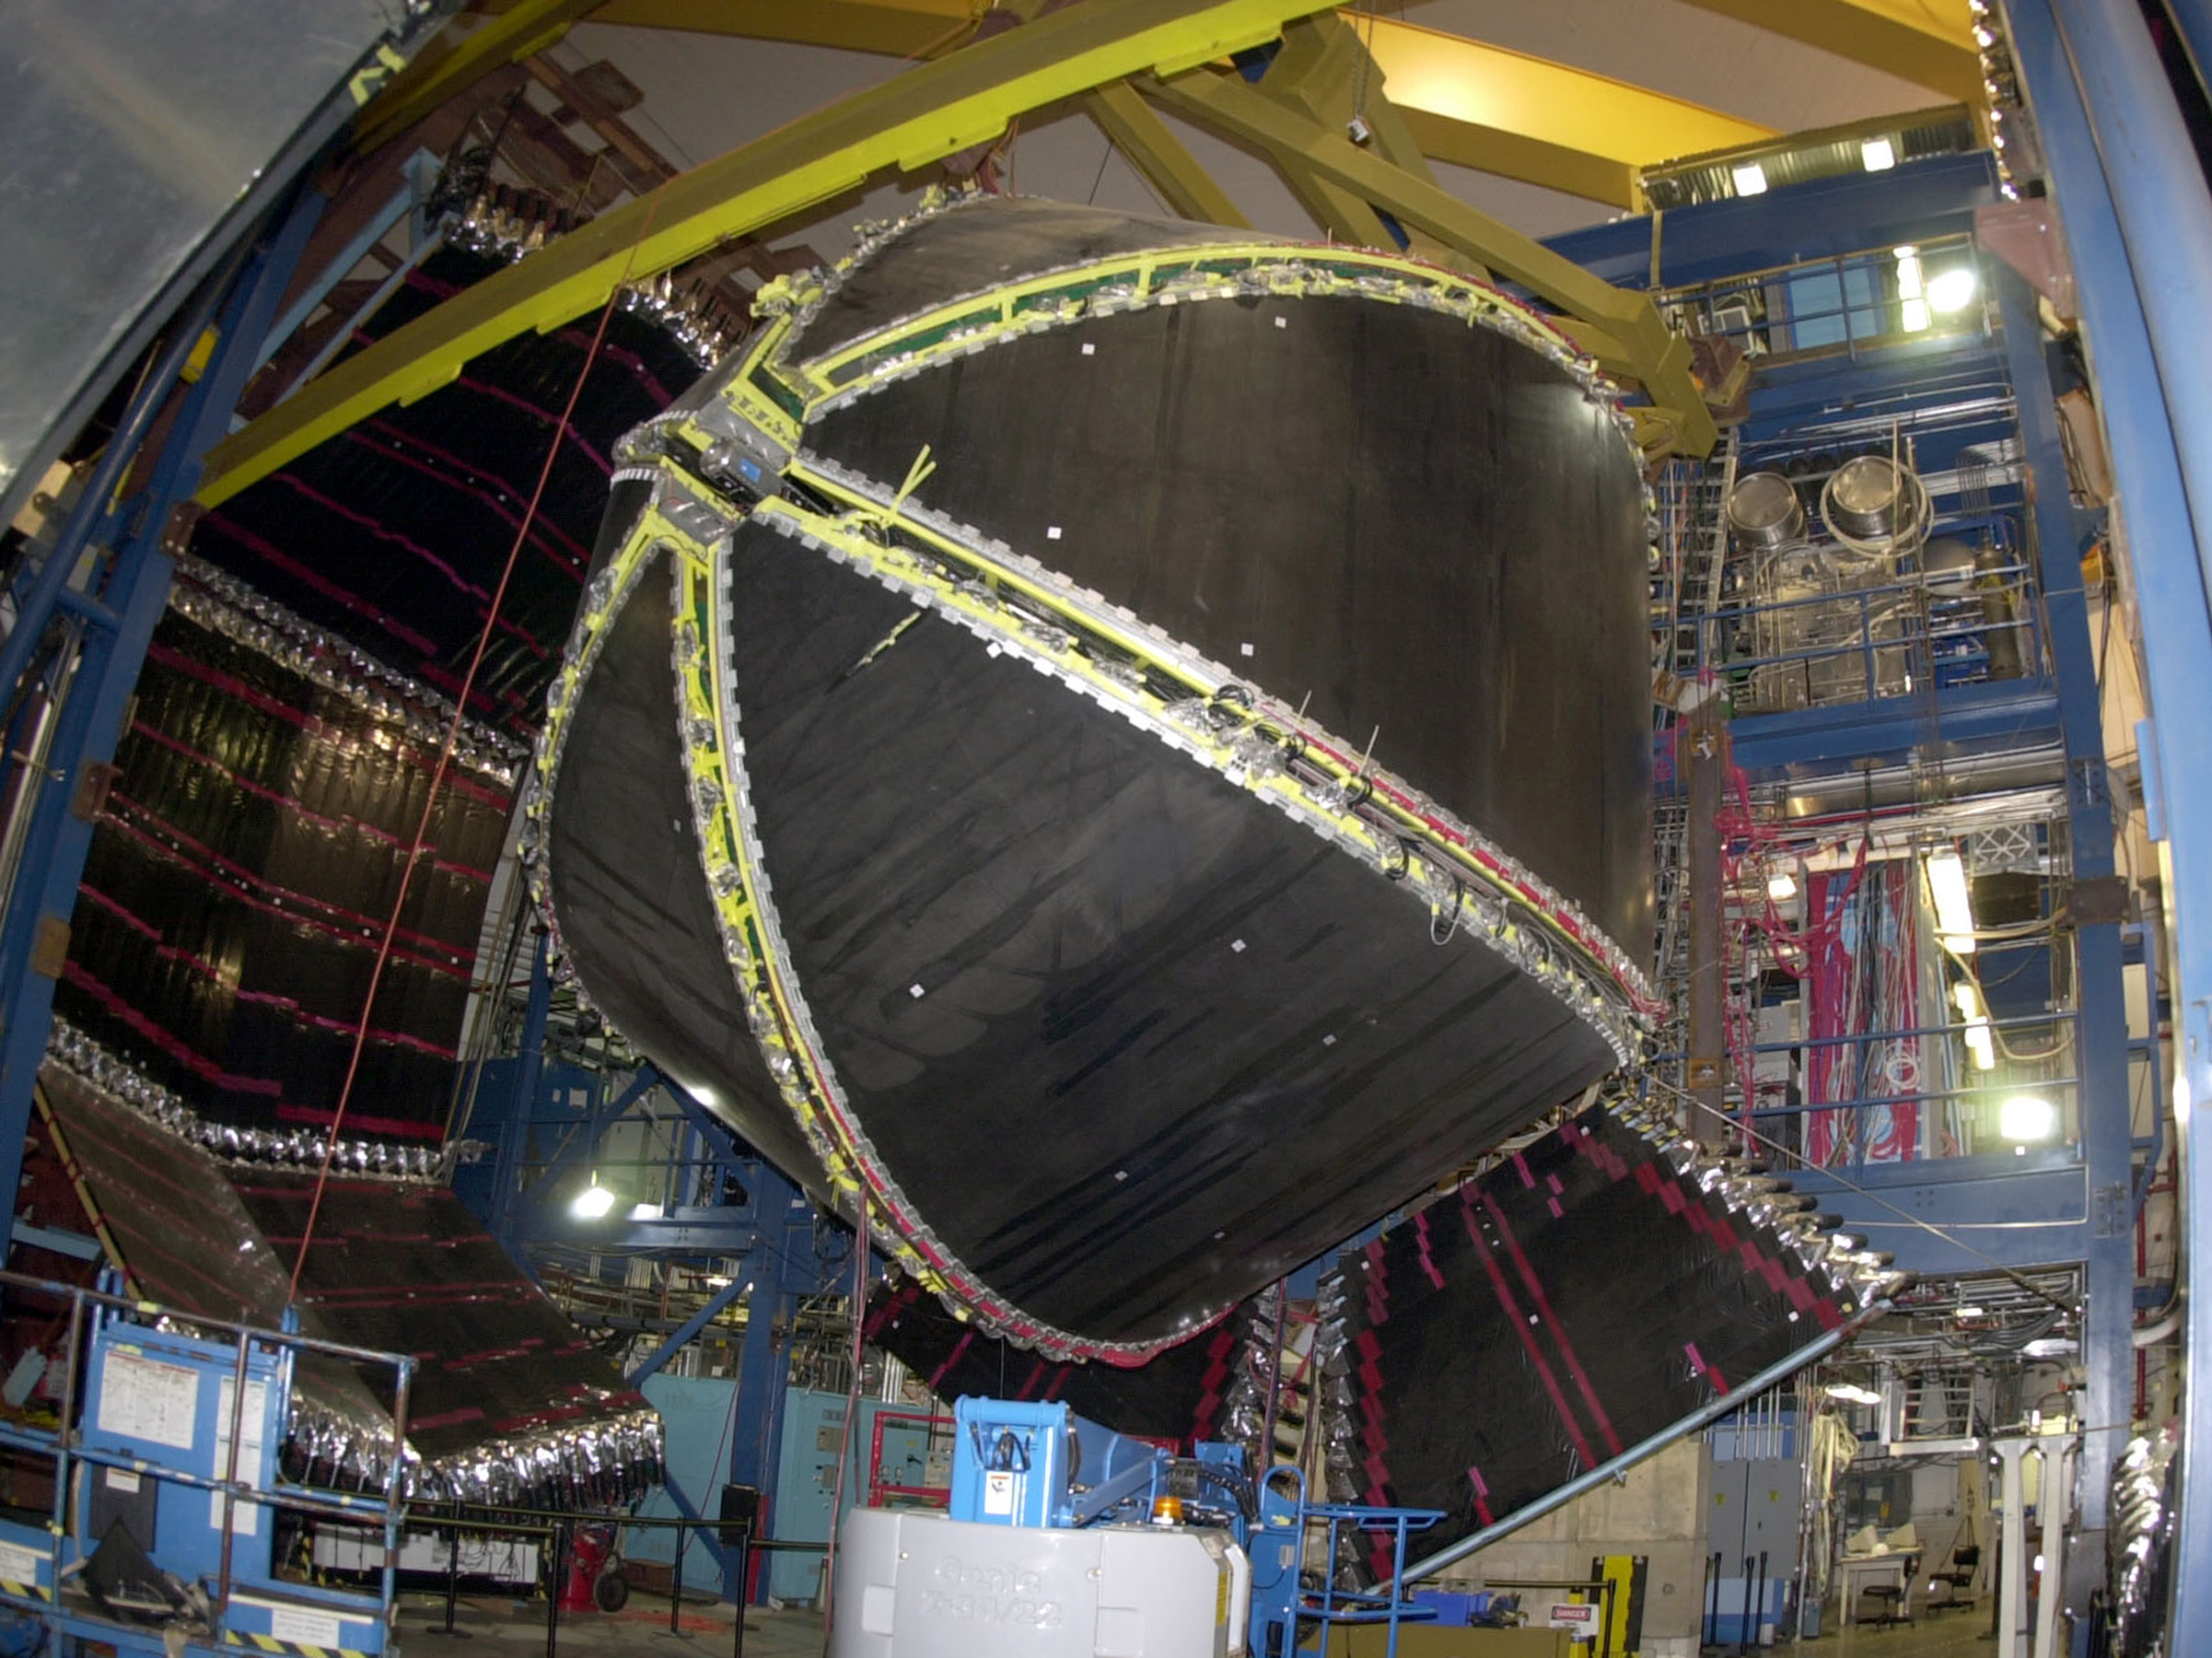
\includegraphics[width=0.6\textwidth]{ImgChap1/CLASPhoto}
	\caption{Photograph of the CLAS detector.}
	\label{CLASPhoto}
\end{figure}

The magnetic field in CLAS is generated by 6 superconducting coils that are arranged symmetrically around the beamline at $60\textdegree$ intervals. These produce a field primarily orientated in the $\theta$-direction perpendicular to the beamline.

\begin{figure}
	\centering
	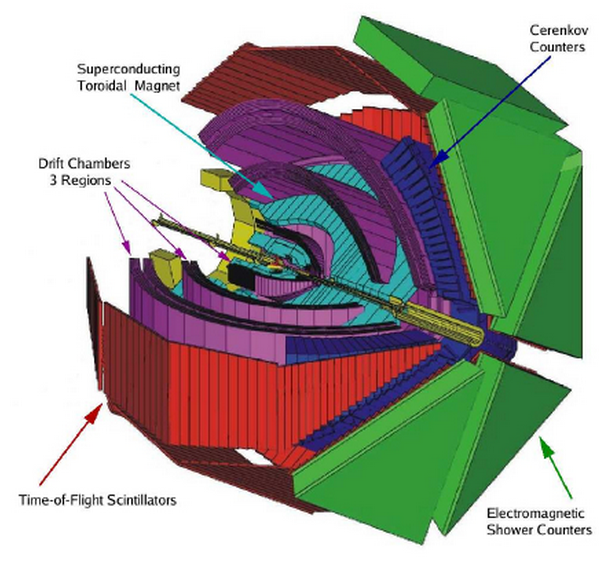
\includegraphics[width=0.6\textwidth]{ImgChap1/CLAS1}
	\caption{Schematic picture of CLAS with the different subsystems highlighted in colour. \textbf{CITATION}}
	\label{CLASDiagram}
\end{figure}

The detector makes use of drift chambers to determine the trajectories of particles. \cite{mestayer2000clas} Gas cherenkov detectors to differentiate between electrons and pions in the detector. \cite{adams2001clas} Scintillation counters for measuring the ToF of particles through the detector. \cite{smith1999time} Finally two types of electromagnetic calorimeters to determine the characteristics of the particle showers and measure the energy deposited. Forward \cite{amarian2001clas} and large angle \cite{anghinolfi2000response}.

The design means the detector is essentially composed of 6 independent magnetic spectrometers working in unison. With each sharing a common target, trigger and readout mechanism. The detector is designed to be suitable for both electron and photon beam experiments, however adjustments are made for different beam conditions. When are electron beam is in use, a 'mini-torus' is added around the target to shield the inner most drift chambers from electrons produced through M\o{}ller scattering in the target. For photon beams a start counter is added inside in the inner drift chambers to provide precision timing for reactions. \cite{taylor2001clas}


%CLAS paper \cite{mecking2003cebaf}
%
%Drift chambers for to determine the trajectories of charged particles \cite{mestayer2000clas}
%
%Gas cherenkov detectors for electron indentification \cite{adams2001clas}
%
%scintillator counters for measuring time of flight \cite{smith1999time}
%
%electromagnetic calorimeters to detect showering particles.
%Forward \cite{amarian2001clas}
%large angle electronmagnetic calorimeter \cite{anghinolfi2000response}

%Detector suitable for both electron and photon beam experiments, however a adjustment is made for the different beam conditions.
%For an electron beam a 'mini-torus' is added around the target to shield the inner most drift chambers from electrons produced through M\o{}ller scattering in the target.
%
%Start counter used for tagged-bremsstrahlung experiments \cite{taylor2001clas}

\subsection{Tagged-Bremsstrahlung}

In CLAS photon beams are produced through by passing the CEBAF electron beam through a thin target (the "radiator") positioned just upstream of a magnetic spectrometer (the "tagger") The system uses electron bremsstrahlung reactions during which an incident electron of energy $E_{0}$ is scattered by the electromagnetic field of a nucleus, causing an energetic photon to be released. The energy transferred to the nucleus during the reaction is negligibly small, so the energy conservation reaction can be written as

\begin{equation}
E_{\gamma} = E_{0} - E_{e}
\end{equation}


Where $E_{\gamma}$ is the energy of the photon and $E_{e}$ is the energy of the post-reaction electron. From this if the energy of the electron beam is known. Then the energy of the photon can be resolved from determining the energy of the scattered electron in a magnetic spectrometer. \cite{sober2000bremsstrahlung}

\begin{figure}
	\centering
	\includegraphics[width=0.9\textwidth]{ImgChap1/Brem1improved}
	\caption{Diagram of the bremsstrahlung production mechanism and the spread of electron energies measurement which allow the energy of the photon beam to be resolved. \cite{sober2000bremsstrahlung}}
	\label{CLASbrem}
\end{figure}

The production angle of the photon is dependent on beam energy and at energies great than a few MeV the photon and electron emerge at angles little deviated from the beam direction. The scatter angle of the photon is also dependent on the rest of the electron $m_{e}$ and follows the relation

\begin{equation}
\theta_{\gamma} = mc^{2} / E_{0}
\end{equation}


The corresponding scatter angle of the electron is given by

\begin{equation}
\theta_{e} = \theta_{\gamma}E_{\gamma} / E_{e}
\end{equation}

At the energies utilised at Jefferson Lab, both of these angles are of the order of 1 mr or smaller. To a first approximation it can be taken that the photon and electron travel in the same direction as the original beam. The produced photons pass through the field produced by the tagger magnet continue on towards the beam target. These are further constrained by a series of collimators placed just downstream of the tagger. Details of this mechanics and the structure of the tagger are shown in Figures \ref{CLASbrem} and \ref{CLASbrem1}.

The strength of the tagger magnet is adjusted depending on the beam energy to ensure those electrons that do not radiate will follow an arc directly into a shielded beam dump. Those that do will follow a tighter arc with a spread dependent on the percentage of incident energy transferred to the photon and the strength of the tagger field. A flat plane segmented scintillator hodoscope is positioned to cover the arc of electrons covering an energy range of $20\%$ to $95\%$ of the electron beam energy. This requires sufficient segmentation to provide adequate energy resolution and fast enough timing resolution to be able to separate the 2 ns separated beam bunches. In order to minimise the effects of re-scattering the electrons are pass through a thin exit window just after scatting into a vacuum chamber until they reach the scintillators. \cite{sober2000bremsstrahlung}


\begin{figure}
	\centering
	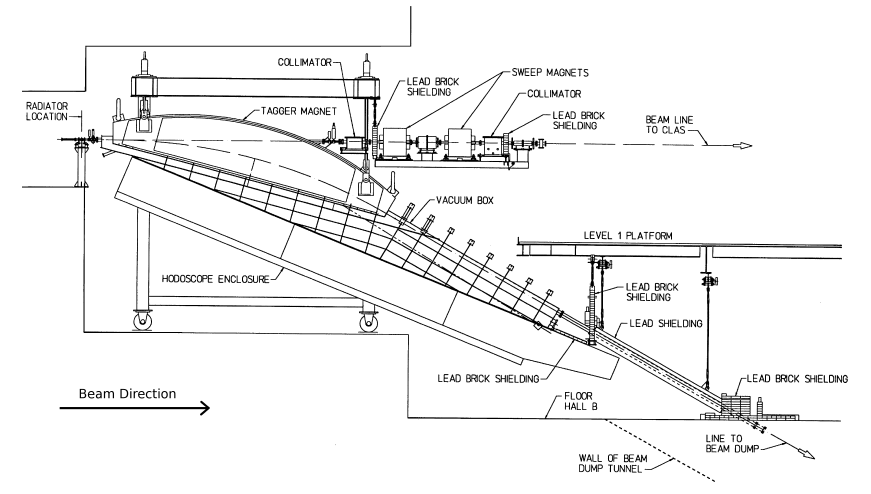
\includegraphics[width=0.9\textwidth]{ImgChap1/BremFac}
	\caption{Diagram of the contruction of the bremsstrahlung production mechanism. In particular highlighting, the radiator, vacuum chamber and collimator positioning. \cite{sober2000bremsstrahlung}}
	\label{CLASbrem1}
\end{figure}


\subsection{Detectors Systems}


\subsubsection{Torus Magnet} \cite{street1996final} \cite{o1989superconducting}

The magnetic field required for momentum analysis within CLAS is generated by 6 superconducting coils arranged in a toroidal shape around the beamline. The combined arrangement forms a system of $\sim$5m in length and and 5m in diameter. The symmetric design produces a magnetic field which is primarily focused in the $\phi$-direction, with some deviation close to each of the magnetic coils. Whilst also maintaining a largely field free region in the centre of the detector region allowing for the operation of a polarized target. Figure \ref{MagneticFields1} shows the vectors of the magnetic field from the viewpoint along the beamline. The length of the vectors are proportional to the strength of the magnetic field at each point.

\begin{figure}
	\centering
	\includegraphics[width=0.6\textwidth]{ImgChap1/meson2}
	\caption{Torus magnets.}
	\label{CLAStorus}
\end{figure}

\begin{figure}
	\centering
	\includegraphics[width=0.6\textwidth]{ImgChap1/mag}
	\caption{Torus magnets.}
	\label{MagneticFields1}
\end{figure}

Each of these coils that form the system is kidney shaped producing a field which more strongly effects particles scattered at forward angles (with typically higher momentum) with more limited effects at wider scatter angles. At the maximum design current of 3860 A, the integral of the field strength of forward angles reaches 2.5 T at forward angles dropping to 0.6 T at a scatter angle of $90\deg$. Field lines of equal strength are shown in Figure \ref{MagneticFields2} from a perspective between two of the superconducting coils.

\begin{figure}
	\centering
	\includegraphics[width=0.6\textwidth]{ImgChap1/mag1}
	\caption{Torus magnets.}
	\label{MagneticFields2}
\end{figure}

\subsubsection{Drift Chambers} \cite{mestayer2000clas} \cite{carman1998region} \cite{qin1998prototype}

The magnetic field generated by the coils bends charged particles either away or towards the beamline, with minimal effect in the azimuthal direction. The particles trajectories by a 6-way symmetric arrangement of 18 drift chambers split into 3 'regions' (R1, R2 and R3) matching the natural geometry arising from the arrangement of the 6 superconducting coils. The R1 drift chambers are positioned just outside the target area in a region of low magnetic field. The R2 drift chambers are positioned between the magnetic coils in an area high field near the point of maximum sagitta for the charged particles. The R3 chambers are positioned outside the magnetic coils in a region of lower magnetic field. Their relative positions and orientations are shown in Figure \ref{CLASdrift}.

\begin{figure}
	\centering
	\includegraphics[width=0.6\textwidth]{ImgChap1/meson2}
	\caption{Drift Chambers positions.}
	\label{CLASdrift}
\end{figure}

For optimal coverage and maximum sensitivity to the radius of curvature, the drift chambers are positioned between each of the magnetic coils at $60\deg$ intervals approximately perpendicular to the bend plane. The chambers fill the wedge shape detector volumes with field and sensing wires spaced to form a series 'layers' of concentric partial circles with wires in each layer positioned half a wire diameter along from the next. Forming an arrangement similar in geometry to hexagonal close packing throughout the detector volume. This is shown clearly in Figure \ref{CLASdriftwires}. The size of the hexagonal structures increases in proportion to the distance from the centre of the detector.

\begin{figure}
	\centering
	\includegraphics[width=0.6\textwidth]{ImgChap1/meson2}
	\caption{Drift Chambers positions.}
	\label{CLASdriftwires}
\end{figure}

For improved tracking and azimuthal information, each drift chamber is split into two 'superlayers', one axial to the magnetic field and the other with a $6\deg$ tilt to provide stereo azimuthal information. An exception to this is R1, due to space limitations it has only a single axial layer. 

For safety and detector longevity reasons the wires chambers are filled with a $88\%-12\%$ mix of argon and $CO_{2}$ which is controlled by an active feedback systems which maintains constant system conditions adjusting for any changes in the surrounding environment. 

The detector resolution is dependent on single wire resolution along with uncertainties from multiple scattering in the material, the true value of the magnetic field strength and misalignments in the geometry of the detector system. Single wire resolution is dependent on where within the cell a track passes. With increasing uncertainty when close to either the sensing or field wires and improved resolution towards the middle of each cell. This is due to ion-pair production near the sensing wire and divergence of the magnetic field and time walk affects near the field wires in a cell. The resolution for a track pathing in the mid region of a cell is 200-250 $\mu$m. With a whole cell average of $\sim$ 310, 315 and 380 $\mu$m for R1, R2 and R3 respectively. \cite{mecking2003cebaf} 


\subsubsection{Cerenkov Counters}

\cite{adams2001clas}

The Cerenkov counters serve the dual purpose of differentiating between electrons and pions and providing a trigger on electrons. They are designed to maximise the solid angle coverage in each of the six sectors up to $\theta = 45$ whilst using the minimum amount of material (To limit its effect on energy resolution). This is achieved by placing the Photomultiplier tubes and light collection cones in regions in $\phi$ which are already shadowed by the structure of the toroidal magnets and covering as much of the solid angle as possible with mirrors. Figure \ref{CLAScerenkov} shows the layout of one of the Cerenkov detectors.

\begin{figure}
	\centering
	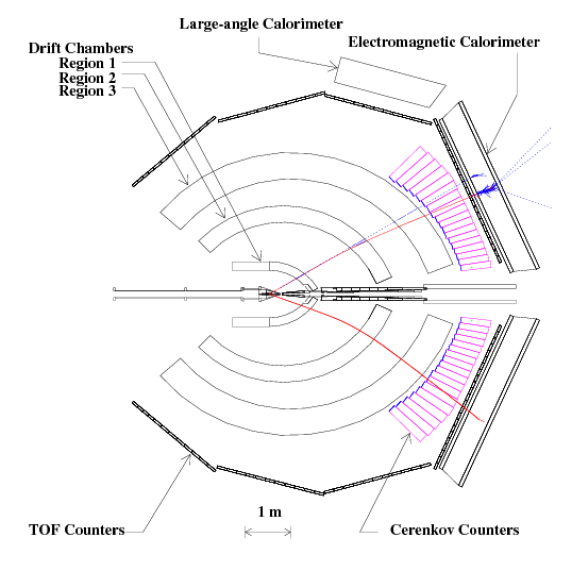
\includegraphics[width=0.6\textwidth]{ImgChap1/CLAS2}
	\caption{Cerenkov layout, get a better picture, that shows the structure of the Cerenkov.}
	\label{CLAScerenkov}
\end{figure}

Coverage of $\theta$ in each of the six sectors of CLAS is divided into 18 regions and each of these was further subdivided into two modules bisecting the centre of each of the 6 sectors. Resulting in a total of 12 identical subsectors about the $\phi$-axis for each of the 18 sections in $\theta$ for a total of 216 Cerenkov modules. \cite{adams2001clas}

\subsubsection{Time of Flight Counters}

This detector system covers the azimuthal angle $\phi$ between $8\deg$ and $142\deg$ and works in conjunction with the start counter, when using photon beams, to determine the time of flight of particles (ToF) within CLAS. Particles propagating radially outwards from the target will reach the ToF counters after passing through the drift chambers and at forward angles also the Cerenkov counters.

The detectors are composed of Bicron-408, a fast responding plastic scintillator, in sections 5.08cm thick, designed to produce signals of large amplitude from minimum ionising particles passing through the detector. Each scintillator block is positioned to be perpendicular to the mean propagation direction of reaction products, covering $\sim 1.5 \deg \theta$. The forward angle counters ($\theta < 45$) are 15 cm wide, and those at wider scattering angles are 22 cm wide in the $\Delta\theta$ direction. The forward angle counters are between 32 and 376 cm in length and the wide angle detectors are 371 to 445 cm in length, with timing resolutions of between $\sim 90-160 ps$ For scintillators of these dimensions the dominant contribution to timing resolution is the varying path length of photons produced in the materials on their way to the PMTs. The spread of these is shown in Figure \ref{CLAStof} For further information on the ToF counters see \cite{smith1999time}.

\begin{figure}
	\centering
	\includegraphics[width=0.6\textwidth]{ImgChap1/meson2}
	\caption{Spread of timing resolution for the ToF detectors.}
	\label{CLAStof}
\end{figure}

\subsubsection{Electromagnetic Calorimeters}

CLAS utilises a Forward Electromagnetic Calorimeter (FC) that covers its full acceptance range in $\phi$ and up to $\theta$ = $45\deg$ and an additional Large Angle Electromagnetic Calorimeter (LAC) that covers 2 of 6 sectors of CLAS in the range $\theta$ = $45\deg-75\deg$. This section will focus on the main FC but the LAC has a similar design and additional detail can be found in \cite{anghinolfi2000response}. The main functions of the FC detector system are identification and triggering of electrons above 0.5 GeV, detection of photons above 0.2 GeV, (For reconstruction of $\pi^{0}$ and $\eta$) and neutron detection. It covers a range up to $\theta$ = $45\deg$ and is constructed from alternating layers of lead and scintillator in a 0.24 ratio. 

The system is split into 6 sectors positioned between the coils of the torus forming a shape approximating an equilateral triangle. There are 39 layers in the detector system, comprised from 10mm of scintillator followed by 2.4 mm of lead. These layers follow a "projective" geometry directed towards the nominal target position, with each subsequent layer progressing radially outwards, covering a linearly increasing area.  Each layer is composed of 36 strips rotated through $120\deg$ with respect to the previous layer and readout at one of the three edges of each sector. Depending on their orientation the 39 layers are split into 3 groups (U,V and W) to provide stereo information on the location of the energy deposited. These groups are further subdivided into an inner (5 layers) and outer (8 layers) stack for greater longitudinal information to improve hadron and electron separation.

\begin{figure}
	\centering
	\includegraphics[width=0.6\textwidth]{ImgChap1/meson2}
	\caption{Picture of the forward EC and the LAC.}
	\label{CLASForwardEC}
\end{figure}

Hit reconstruction requires a hit in U,V and W layers of the detector in either the inner or outer potions of a sector. Positions are calculated by reconstructing the intersection points of strips triggered above threshold, weighting appropriately for the timing an energy response depending on the position of the hit in the detector system. Hits recorded within 10cm of the edge of the detector volume are discarded to ensure the full electromagnetic shower is contained within the sensitive region of the detector. Using electrons as an example for the performance of the detector; for those above 3 GeV the sampling fraction of the system is $\sim 0.3$. Below this the rate decreases falling to 0.25 for electrons of 0.5 GeV. For electron showers that deposit more than 0.5 GeV in the scintillator the rms position resolution is $\sim 2.3 cm$. Finally, the timing resolution for electrons averages 200 ps across the detector system. For further information on the forward electromagnetic calorimeter see \cite{amarian2001clas}.

\subsubsection{Start Counter}

%General overview of the subsystems of clas
%Calorimeters
%Drift Chambers
%Start Counter
%Magnets
%etc

\section{The upgrade to CLAS12}
System upgrades
System additions like the forward tagger covering the forward angle of the beamline.

What the upgrade will mean for the physics programs in Hall B.
\chapter{The Forward Tagger}

\section{The MesonEx Program}

\subsection{The MesonEx Program}
Meson spectroscopy
Quark model describes baryons and mesons as bound states of 3 quarks and a quark anti-quark pair. Desbribes well many of the features of the hadron spectrum. However recent developments have shown that the hadron mass cannot simply me describes in terms of the masses of the constituent quarks, but it mainly due to the dynamics of the interacting gluons that bind the system together. The simpler 2 or 3 quark bound state desciptions is a simplification of the much more complex ever evolving quark-gluon plasma present in all hadrons. Studying the spectrum of hadrons and measuring the properties to learn more about their inner stucture is crucial in developing a deeper understanding of the mechanics of the strong nuclear force.


\textbf{Notes for the rest of the section} 

Mesons, composed of a quark and a anti-quark pair, are the simplest bound quark state and form an ideal environment to study the interactions within hadrons. 
Study confinement.
The role gluons play in QCD.
Quark model predicts the existence of multiplets of mesons with differentiated by the properties of total angular momentum J, parity P and charge conjugation C.
Most of the lowest mass states have been identified and studied.
Some issues still remain.
Models of QCD and lattice calculations predict that states beyond a simple $q\bar{q}$ configuration such as tetraquarks$(qq\bar{q}\bar{q})$, hybrids (qqg)and glueballs, should also exist.
If this is the case we should expect to see a much richer and varied spectrum of hadronic states than is predicted by the quark model.

\subsection{Electroproduction at very small $Q^2$}
%At 11 GeV/c the previous method of producing real bremsstrahlung photons tagged by a magnetic calorimeter is no longer possible due to the limitations of the existing magnet. Instead the plan is to use quasi-real photons produced when electrons are scattered at very small angles (low $Q^2$). This technique has been previously used 


\section{The Forward Tagger}
A new detector system designed to measure particle properties at forward angles, between 2 and 4.5 degrees from the beamline. It has been designed to optimally detect the properties of electrons scattered at very small angles with an acceptance exceeding $99\%$. \cite{FTTDR2012} The new detector will be placed between the High Threshold Cherenkov Counter (HTCC) and the torus suppport within CLAS, in a limited space at most $\sim$ 40 cm in length, just under 2m downsteam of the (nominal) target position. The detector is composed of three major sub-systems:

\begin{itemize}
	\item	Electromagnetic Calorimeter (FT-Cal)
	\item   Scintillation Counter (FT-Hodo)
	\item   Tracker (FT-Trck)
\end{itemize}

The FT-Cal will detect the electrons, measure the energy of the electromagnetic shower and provide a fast trigger for other detector systems in CLAS. The FT-Trck will measure the scattering angles ($\theta_{e}$ and $\phi_{e}$). The FT-Hodo provides e/$\gamma$ separation and further background reduction by taking measurements in coincidence with the calorimeter.

The limited region available for the detector and the close proximity to the beamline (2.5\textdegree coresponds to $\sim$ 8 cm) necessitates compact detector systems that are able to process the very high flux present while remaining highly resistant to radiation damage. All components are contained with a region \textless5\textdegree from the beamline, to minimize interfere with any of the other systems in CLAS. 

A brief overview of the main subsystems of the detector will be given in the following section before going to explore in more depth the design of the FT-Hodo which is the main focus of this thesis.

\begin{figure}
	\centering
	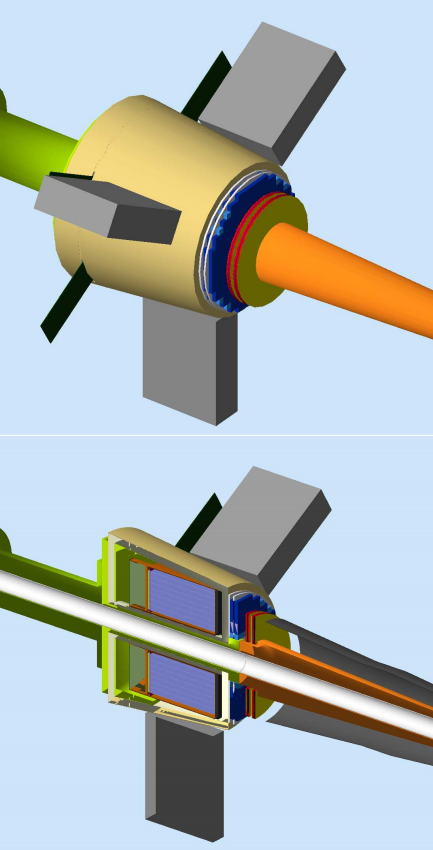
\includegraphics[width=0.6\textwidth]{ImgChap1/FTcross}
	\caption{Cross section of the forward tagger. \cite{FTTDR2012} }
	\label{FTcross}
\end{figure}



%Give some background and context to the work.
%Define the relevence of the area and why there is interesting work to be done there.
%Give some context of the current state of research and where JLAB fits into this.
%Discuss about CLAS, then about CLAS12, then about the forward tagger.
%Go on to discuss the purpose of the hodoscope and overall design contraints.
%General overview of the design key elements of interest.
%Discuss the key decision areas in detail. Tiles, Fibres, SiPMs, Reflective materials etc.
%Discuss the ongoing testing and literature research that lead to the decisions made.

\subsubsection{FT-Cal}
The FT-Cal is a highly segmented lead tungstate based electromagnetic calorimeter that has to fulfil demanding requirements in a limited space. The detector requires, high light yield and a fast recovery time ($\sim$ 10 ns) for high energy resolution and minimal pile up within the detector. Excellent timing resolution for tagger events in conjunction with other systems within CLAS. Finally it requires high radiation hardness, combined with a small radiation length and Moliere radius within the detector.

To achieve these objectives the detector was designed to be highly segmented in the transverse direction to maintain a sustainable output rate from each pixel. In addition the traverse size of each element should be comparable to the typical Moliere radius of the electromagnetic shower produced in the detector. This will minimise unnecessary pixel firing by containing the shower to a limited number of crystals. A simple diagram of the FT-Cal is shown in Figure \ref{ftcalo} with the showing the arrangement of the crystals.

\begin{figure}
	\centering
	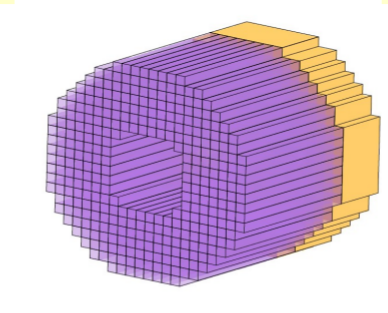
\includegraphics[width=0.6\textwidth]{ImgChap1/ftcalo}
	\caption{A simple schematic of the geometry of the forward tagger calorimeter. With each of the individual lead tungstate crystals highlighted in purple and the readout systems in yellow. \cite{FTTDR2012}}
	\label{ftcalo}
\end{figure}


Lead tungstate ($PbWO_{4}$) has been extensively studied and used in several large scale detectors in recent years. \cite{zhou2007phos,erni2008technical}It was selected for crystals due to its fast scintillation decay time (6.5 ns), a small radiation length (0.9 cm), and limited Moliere radii (2.1 cm). The main disadvantage of the material is its limited light yield ($0.3\%$ of NaI(TI)). However recent improvements to manufacturing processes and cooling of the material below 0\textdegree{C} has shown an improvement in this by a factor of 6-8. With this configuration an energy resolution of $2\% / \sqrt{E(GeV)} \oplus 1\%$ is expected. \textbf{Need to understand this better} \cite{FTTDR2012}

The readout from the detector is required to operate in a high magnetic field excluding standard photomultiplers. Instead Avalanche Photo Diodes (APD) were selected as they have been shown to be both radiation hard and perform well under such conditions. Further information on the design and properties of the FT-Cal can be found in the forward tagger technical design report. \cite{FTTDR2012}.


\subsubsection{FT-Hodo}

The main design objective of the hodoscope is to differentiate between photons and electrons in the calorimeter. The two particles produce indistinguishable electromagnetic showers in the FT-Cal and additional information from the scintiallator tiles in the hodoscope is required. Electrons will be identified by observing near simultaneous hits correlated in both position and time in the FT-Hodo and FT-Cal. To achieve this objective the FT-Hodo must provide highly efficient charged particle detection with similar spacial and timing resolutions to the calorimeter.

The forward tagger comprises a two layered array of fast response plastic scintillator tiles, a thicker layer for improved timing resolution and a thin layer for enhanced background rejection. The positioning of the detector elements in the hodoscope will mirror the layout of the FT-Cal, ensuring uniform coverage across the two detector systems. The restrictive geometry of the volume occupied by the forward tagger precludes the use of standard light guides and photomultipliers. Instead each element is read out using embedded wavelength shifting fibres (WLS) which are flexible and enhance the performance of the readout silicon photomultipliers (SiPM). Similar systems have been used in the past to achieve the sub ns timing resolution required \cite{stepanyan2008clas}. Figure \ref{fthodo} shows a simplistic depiction of the hodoscope in relation to the calorimeter.

\begin{figure}
	\centering
	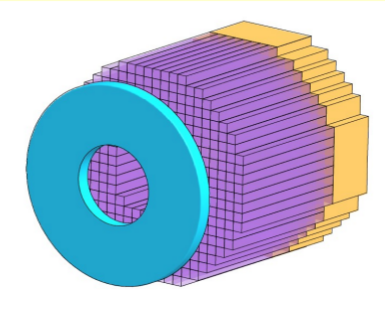
\includegraphics[width=0.6\textwidth]{ImgChap1/fthodo}
	\caption{A simplistic representation of the hodscope, highlighted in light blue, is shown in relation to the calorimeter. \cite{FTTDR2012} }
	\label{fthodo}
\end{figure}

The vast majority of particles incident on the hodoscope will be highly relativistic leaving a fixed minimum ionising deposition in the detector regardless of particle type. As a result having high energy resolution for the energy deposited in each elements is not critical for the detector performance. The main requirements for high detection efficiency and high timing resolution are the number of photons that reach the SiPMs and the efficiency of these detectors to convert these into measurable signals.

%Designed to discriminate between and electrons and photons arriving at the forward tagger with sub nano-second timing accuracy.
%Segmented design composed of two laters of fast responce plastic scintillators coupled by wavelength shifting fibres to Silicon photomultipliers.
%Works in conjuction with the calorimeter and tracker to provide accurate tagging information.
\subsubsection{FT-TrcK}

The role of the FT-Trck is to provide precision positional information to reconstruct the vertex angles of particles entering the forward tagger. It is composed of two doubled layers micromegas detectors with a spatial resolution of $\pm 200\mu{m}$. Each will provide an independent measurement of the (X,Y) co-ordinates and act in conjunction with hits in the hodoscope and calorimeter to improve background rejection. Figure \ref{fttrck} shows the position of the FT-Trck in relation to the FT-Cal and FT-Hodo.

\begin{figure}
	\centering
	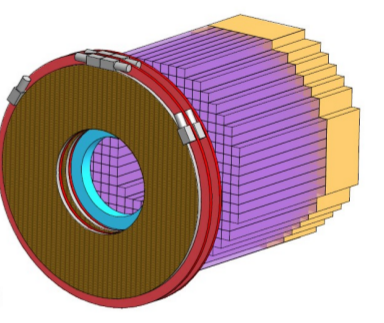
\includegraphics[width=0.6\textwidth]{ImgChap1/fttrck}
	\caption{The three major subsystems of the forward tagger are shown with the FT-trck, highlighted in brown and red, superimposed in front of the FT-Hodo and FT-Cal. \cite{FTTDR2012} }
	\label{fttrck}
\end{figure}

This configuration of the FT-Trck is expected to achieve angular resolutions of $\sim$ 1.7$\%$ and 2.8\textdegree in $\theta$ and $\phi$ respectively.
Further information on the design and properties of the FT-Cal can be found in the forward tagger technical design report. \cite{FTTDR2012}.



\section{Design of the Hodoscope}

This section will discuss in more detail the design of the hodoscope based on the contraints and aims of its construction. Critical points will be highlighted and the interconnected nature of different elements elaborated upon. However deeper discussion into the developmental decisions made and their consequences in the operation of the hodoscope are reserved for Chapter \textbf{TBC} where important sub-systems will be covered in more depth.

As discussed in the previous section the main requirement of the hodoscope is to differentiate between electrons and photons hits in the calorimeter which produce nearly indistinguishable electromagnetic showers. Whilst minimising photon misidentification and suppress false events created through photon conversion. As discussed in \textbf{section SOMETHING} this required a two layered design. The design aims to achieve this with sub-nanosecond timing resolution, to function as part of the trigger system and to not compromise the timing of the calorimeter. It will achieve $>99\%$ particle detection efficiency for the lifetime of its use and achieve this under conditions of high radiation flux and 5T magnetic fields.


The hodoscope is positioned upstream of the FT-Cal fitting within the volume of a circular disk, no more than, 330mm in diameter and 40mm depth. This limited space and harsh operating environment required an innovative approach to its development to optimise the performance of the detector system. However the initial design from which the evolution of the detector design developed is based on proven and tested detector systems. \textbf{Some discussion of literature here?}


Here are general papers on similar detectors.
\cite{reiche2001studies}
\cite{wojcik1994embedded}
\cite{cohn1993scintillating}
\cite{budd2001cms}
\cite{artikov2006new}
\cite{albrow1987uranium}
\cite{barsuk2000fiber}
\cite{adloff2010construction}

The design of the FT-Hodo is based around a segmented array of plastic scintillator tiles (EJ-204) embedded with Wavelength shifting (WLS) fibres (Kuraray Y-11) and read out by 3x3mm Silicon Photomultipliers (SiPM) (Hamamatsu S13360-3075PE). 


\subsection{Plastic Scintillator Tiles}
The plastic scintillators provide fast timing, sufficient light yield and resistance to radiation necessary in the high flux environment of the forward tagger. The limited space, radiation and magnetic fields present in the detector volume required signals to be read out externally. WLS fibres were selected for their flexibility, excellent optical characteristics and radiation resistance. These fibres shift the wavelength of light outputted by the scintillators into the ideal operation range for the SiPMs, however their attenuation length is relatively short at \textbf{<3.5m Check this}. Due to the geometry of CLAS and the enviroment whilst the beam is active the light needs to be transported more than 5m to reach the SiPMs. To resolve this after $\sim$ 10cm, still within the volume of the detector, the WLS fibres are fusion spliced to clear optical fibres which have an attenuation length \textbf{>10m Check this}. This combination allows the scintillation photons to be transported to the readout SiPMs with a light loss of less than $<40\%$. \cite{FTTDR2012}

Each layer of the forward tagger is comprised of 44 15x15mm (P15) and 72 30x30mm (P30) plastic scintillator tiles arranged with 4 fold symmetry about the axis of the beam, covering the same acceptance as the FT-Cal, shown in Figure \ref{hodotilelayout}. At the centre, nearest the beamline, there is a continuous ring of P15 tiles where the flux is expected to be at its highest. Outside this the majority of tiles are P30 type, with each one covering the same area as 4 crystals in the calorimeter. This configuration provides greater resolution in the area of greatest flux while increasing acceptance throughout the rest of the detector. 

\begin{figure}
	\centering
	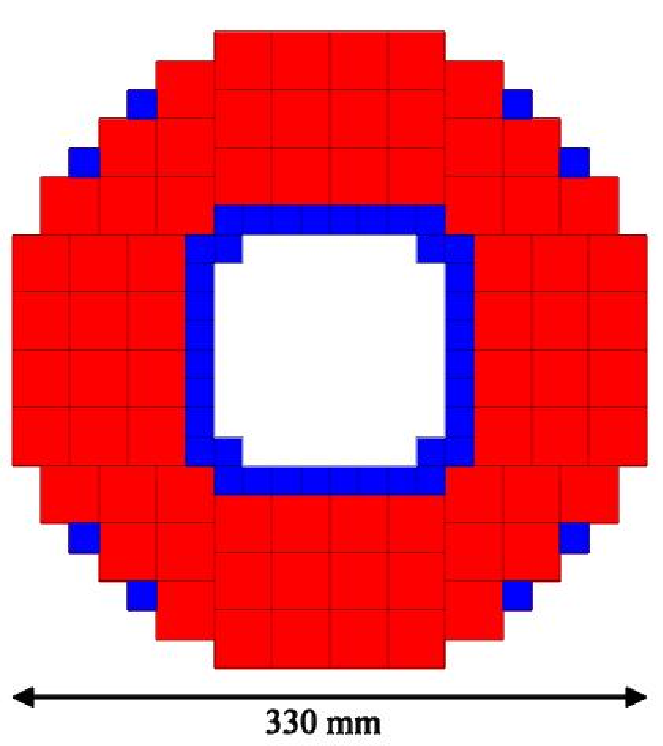
\includegraphics[width=0.6\textwidth]{ImgChap1/hodo}
	\caption{Layout of the plastic scintillator tiles in the hodoscope. 15x15mm elements are shown in blue with 30x30mm elements in red. \cite{FTTDR2012}}
	\label{hodotilelayout}
\end{figure}


\subsection{Wavelength Shifting Fibres}

The photons produced in each of the 116 tiles in each layer of the forward tagger are read out using embedded WLS fibres. These fibres absorb the typically $\sim 400nm$, photons produced in the scintillator tiles and re-emit them in green, $\sim 470nm$ optical range. The ideal operating range for the SiPMs. Each tile has diagonally drilled channels just larger than the 1mm diameter of the fibres, 4 for a P30 tile and 2 for a P15. The channels are aligned to maximise the area fibre length inside each tile, increasing the photon capture cross-section. They also allow for the fibres to feed out naturally from each tile, while maintaining close to complete acceptance of the detector system.  Figure \ref{diagonalholes} shows a photograph of a P30 tile, where the channels can be clearly observed along with the passing of the fibres out from the element.

\begin{figure}
	\centering
	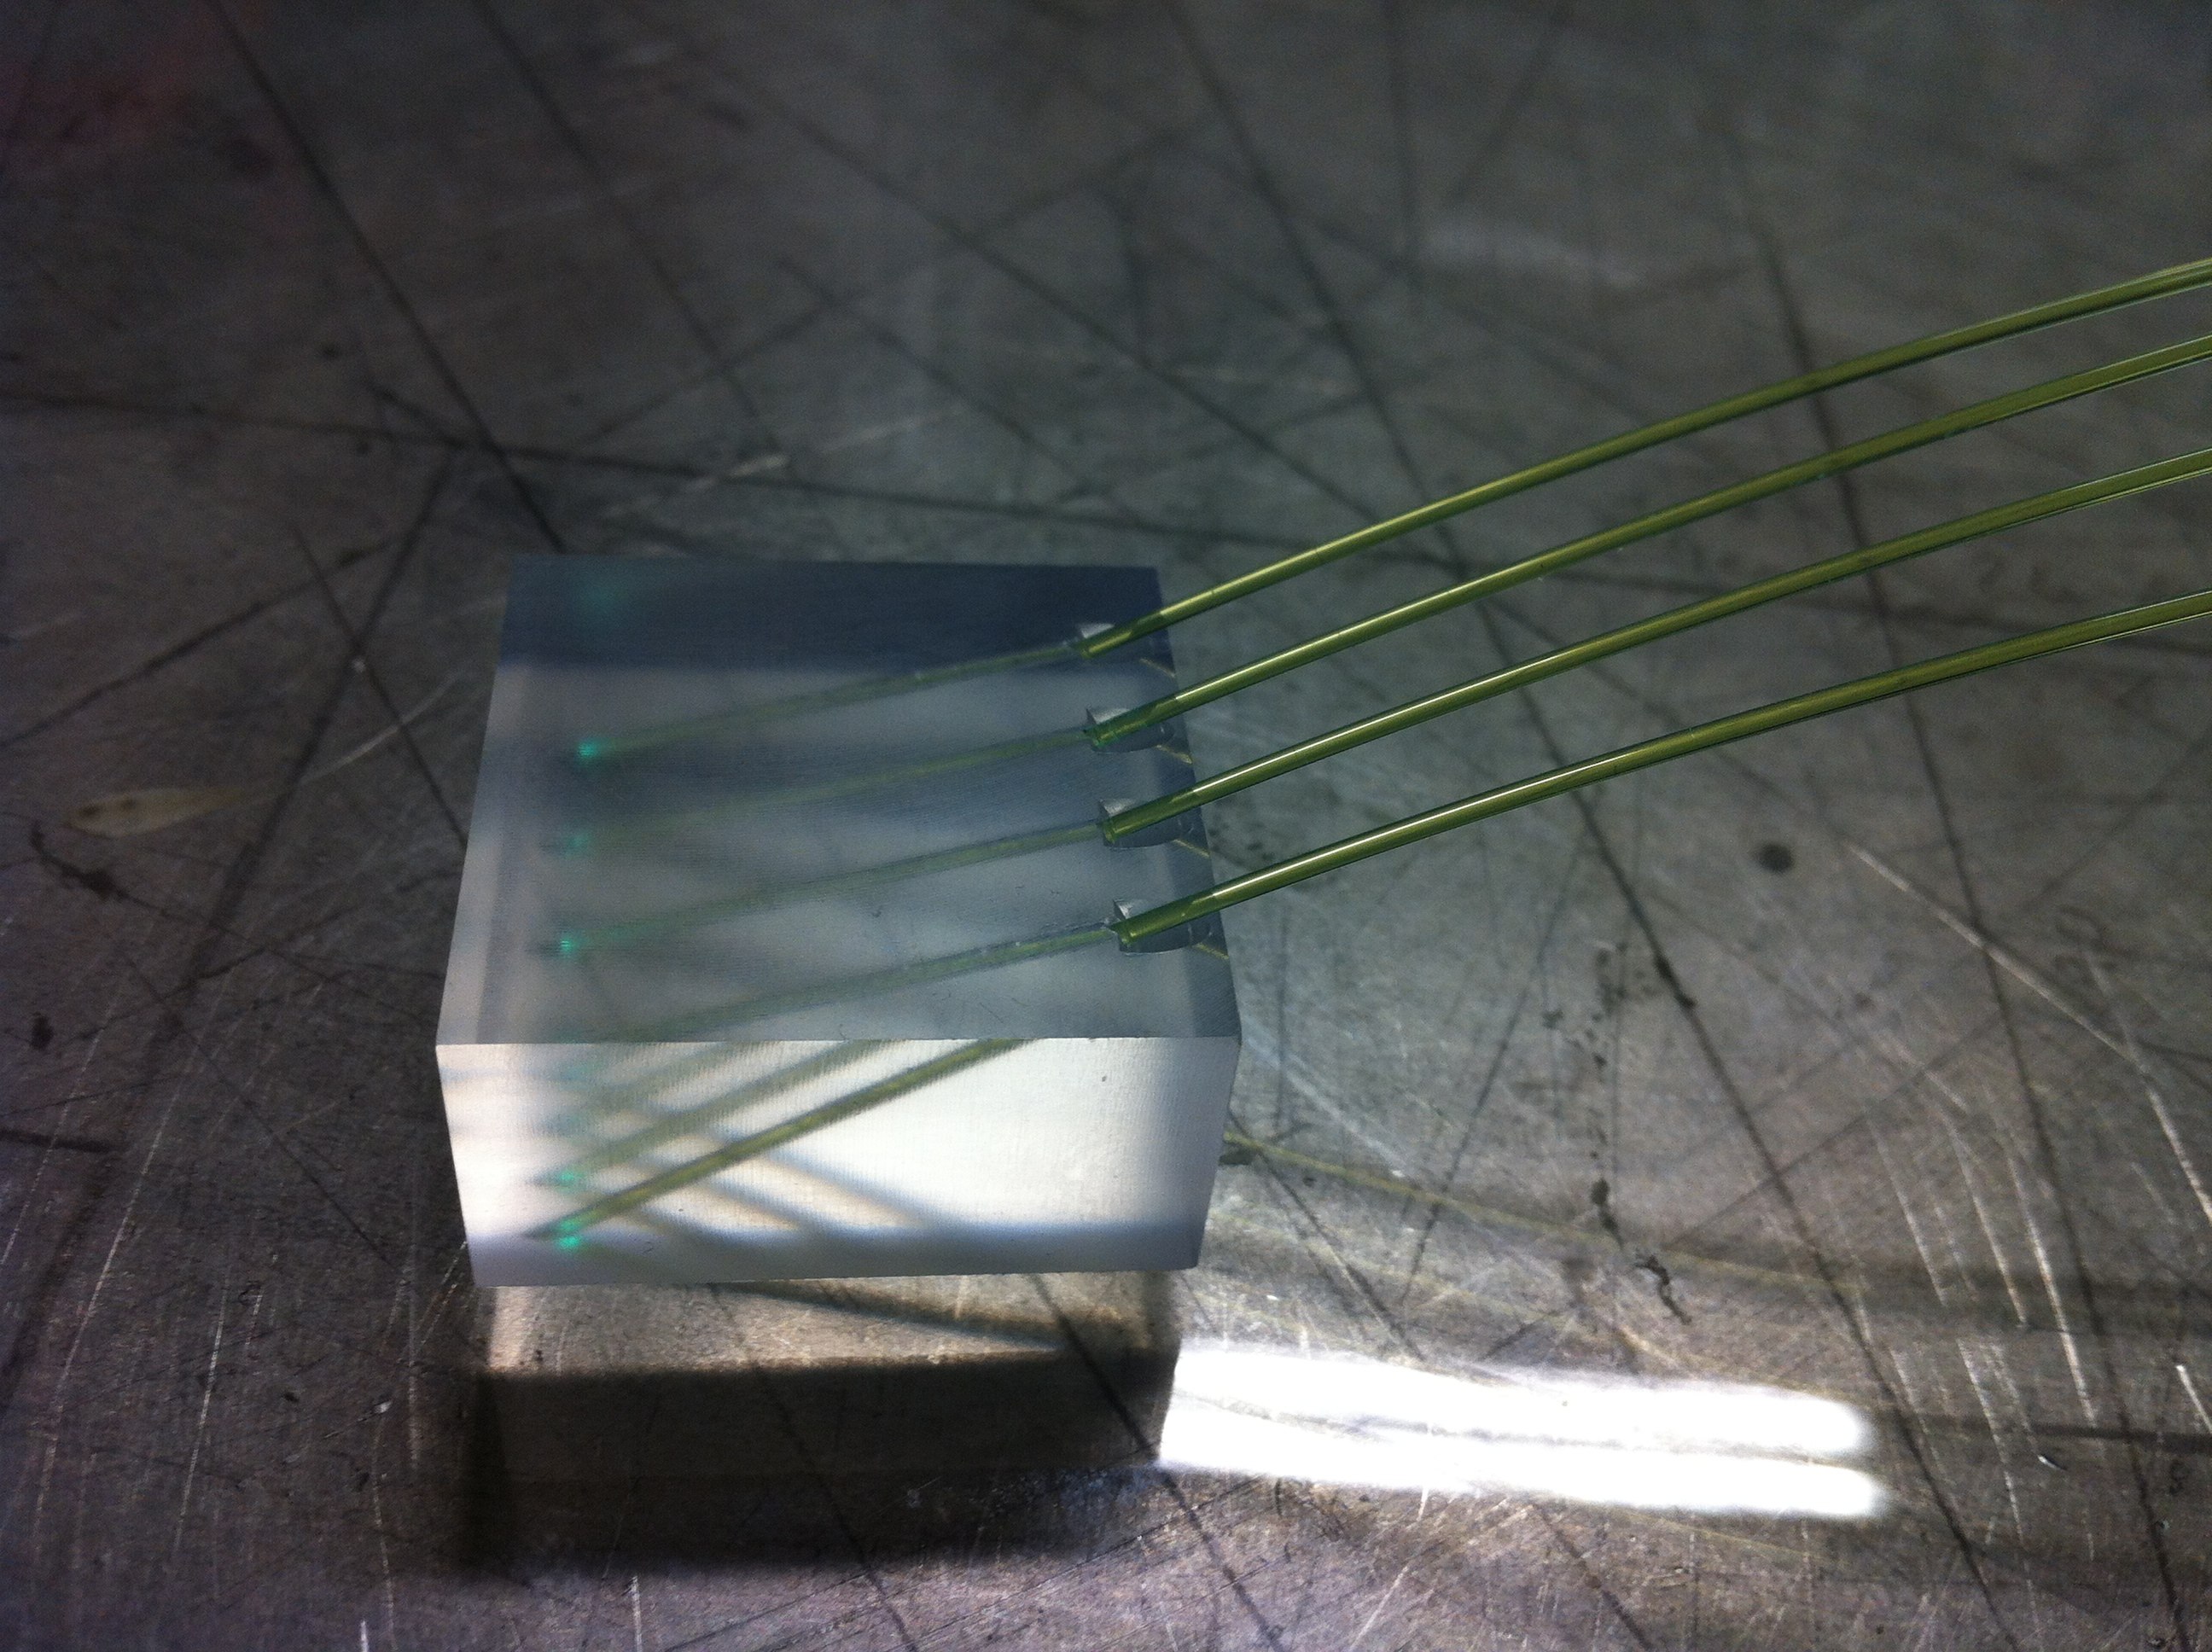
\includegraphics[width=0.6\textwidth]{ImgChap1/diagonalholes}
	\caption{A photograph of an unprepared 15mm thick p30 tiles occupied with 4 wavelength shifting fibres. The diagonally drilled channels for each fibre can be clearly seen.}
	\label{diagonalholes}
\end{figure}

The WLS fibres used in the detector are Multiclad Kuraray Y-11(200) S-Type fibres 1mm in diameter. This type of fibre has shown consistently excellent performance accross a wide array of academic studies. \textbf{need to put in the fibre references here}. The multiclad fibres produce significantly higher lightyield than traditional singleclad fibres as the two layers of differing refractive index outside the core have a much greater photon trapping efficiency. The S-Type fibres were selected for their significantly increased resistance to crasing and transmittance at smalling bending diameters ($<40mm$). This comes at the cost of transparency, leading to a $\sim 10\%$ reduction in attenuation length. Insignificant to the short lengths of WLS fibre used in the detector.

\begin{figure}
	\centering
	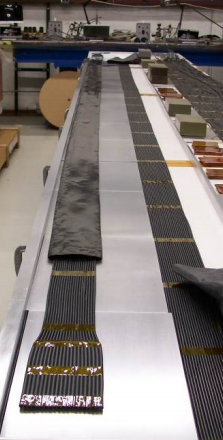
\includegraphics[width=0.5\textwidth]{ImgChap1/fibrelength}
	\caption{A photograph of the full length spliced fibres, put into groups of 4 and placed into protective black PVC sheething.}
	\label{Longfibres}
\end{figure}

The WLS fibres inserted into the tiles are fixed into place using radiation hard optical cement of similar refractive index to the scintillator and fibre. This approach minimises the photon loss across the transition and holds the fibre in place in any orientation of the hodoscope. After 10 cm each WLS fibre is fusion spliced to $\sim 5m $ long section of kuraray doubleclad clear plastic fibre, with again minimal loss of light but now transporting the photons through fibre with much greater attentuation length. This process was carried out at Fermi National Laboratory, with 10cm lengths of WLS fibre spliced to 6m lengths of clear fibre. A photograph of the sliced fibres laid out on laboratory benches is shown in Figure \ref{Longfibres}. 
  
\begin{figure}
	\centering
	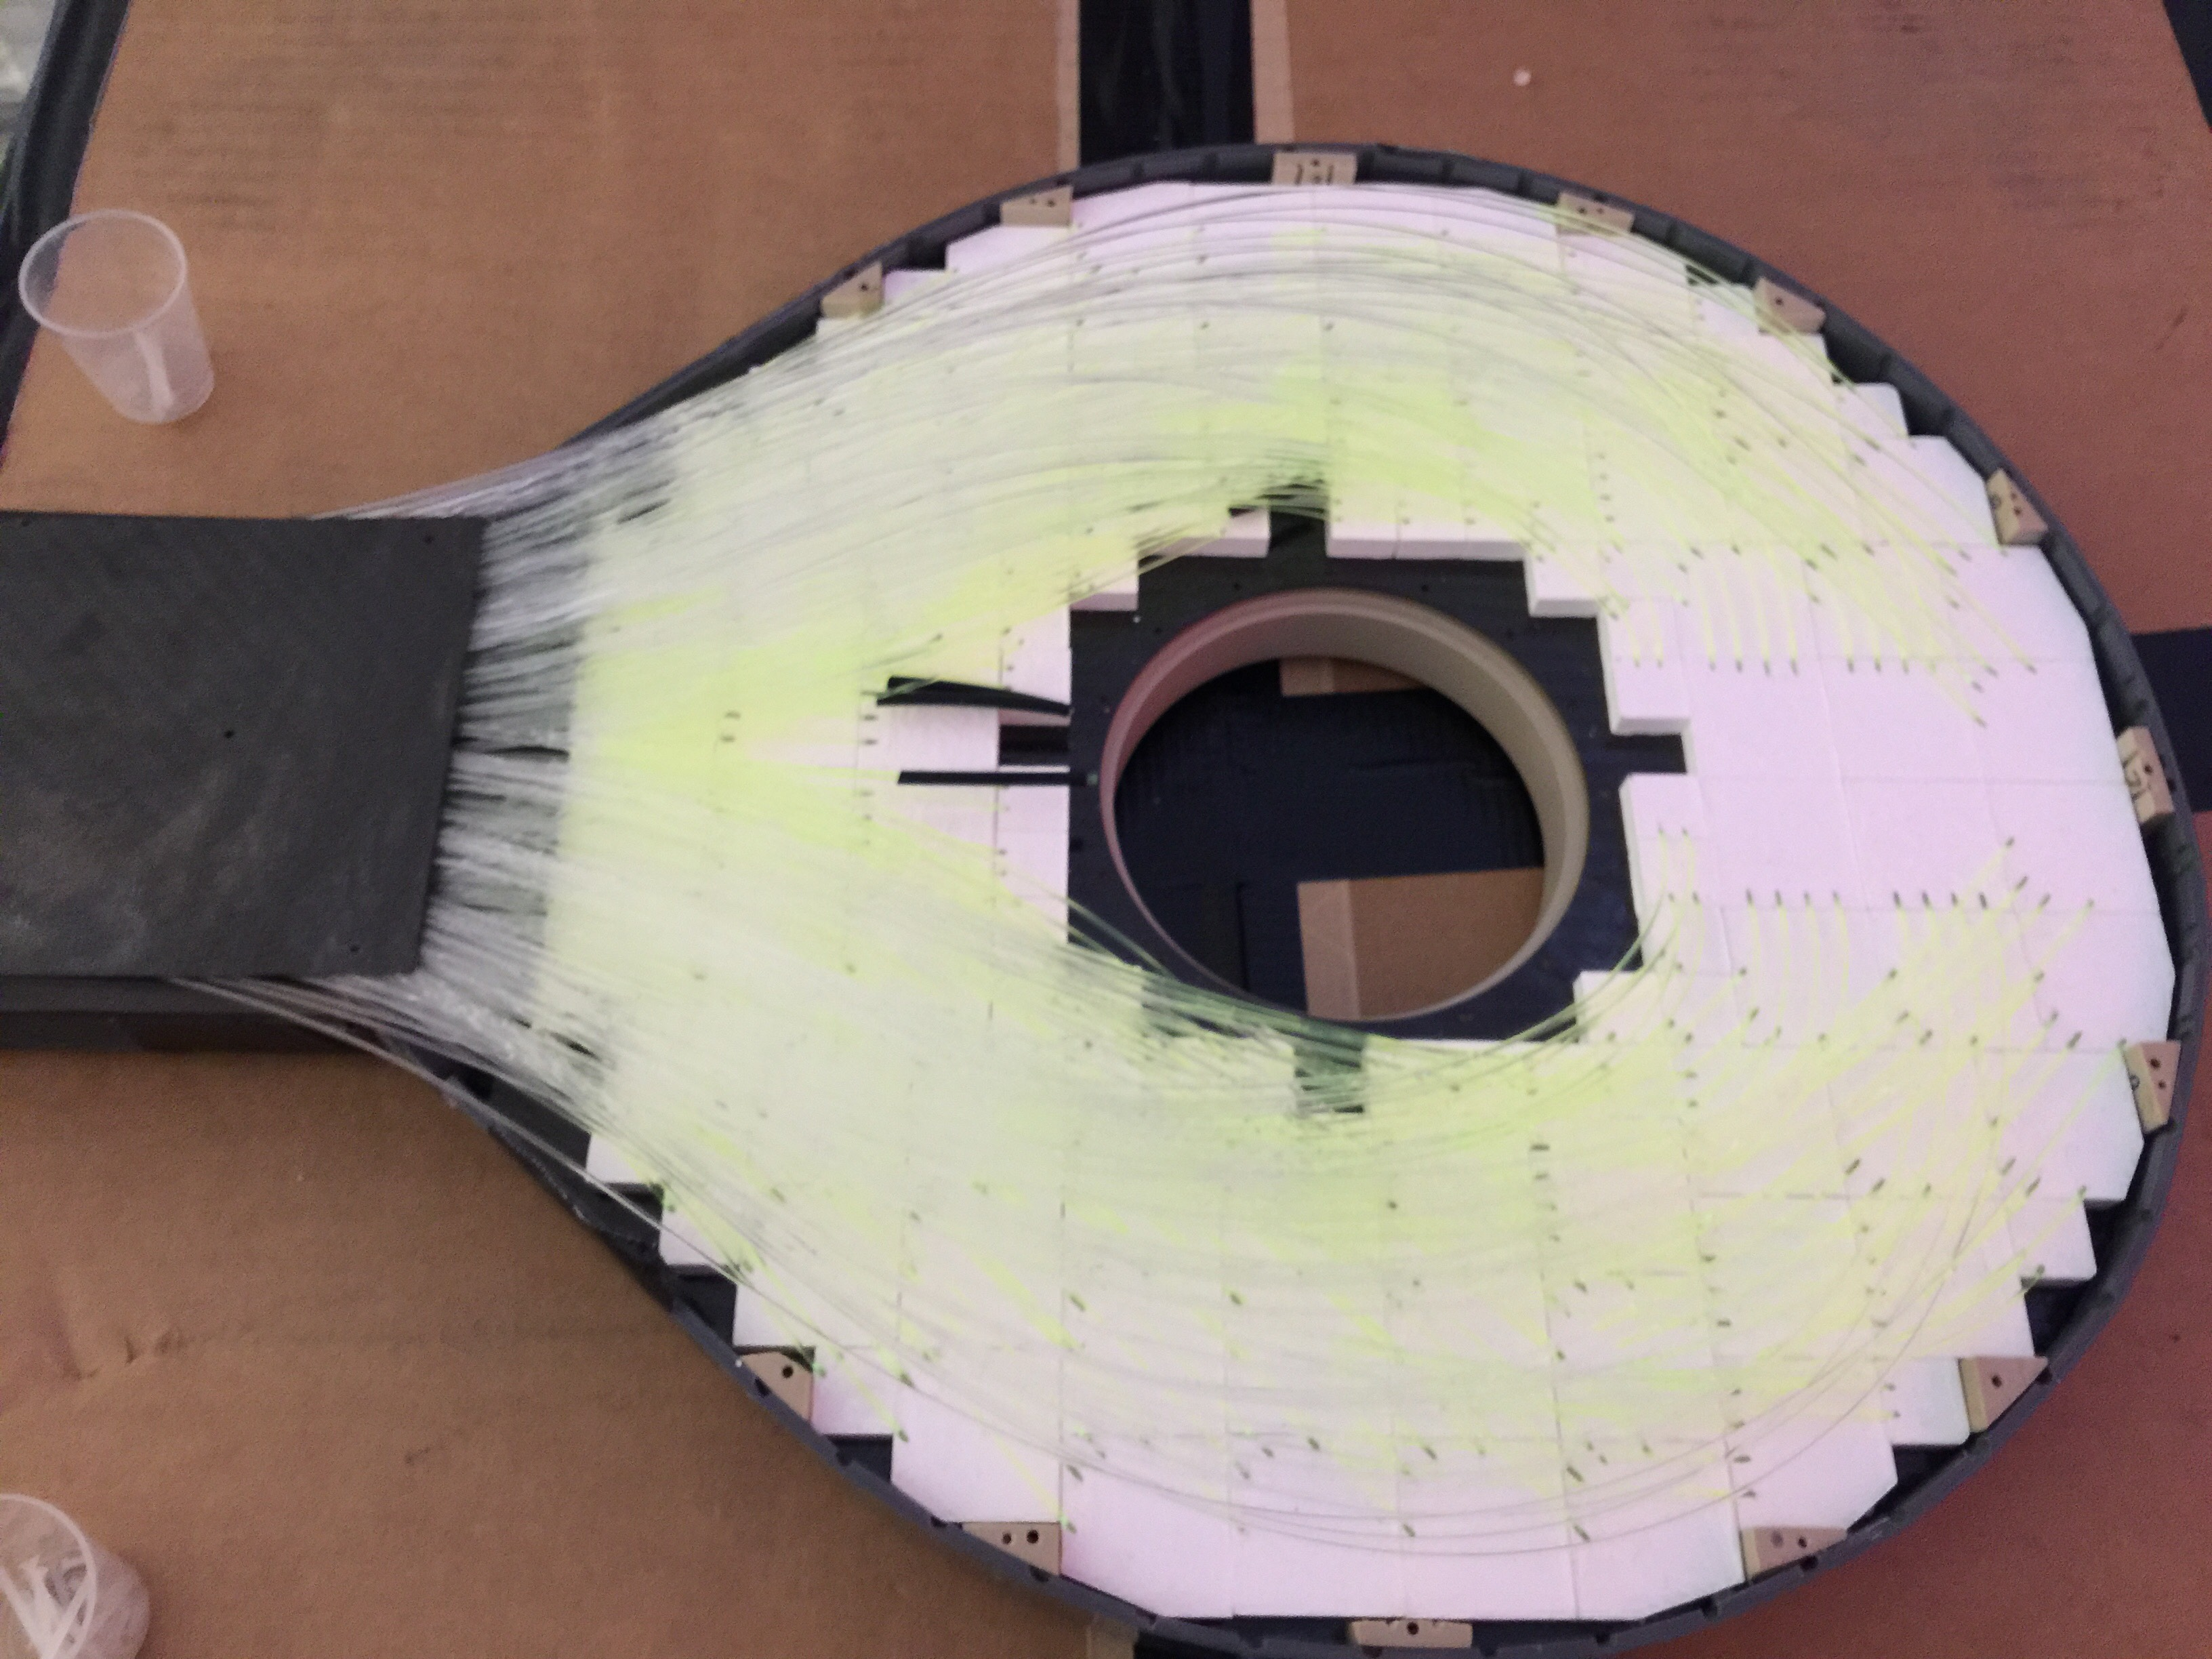
\includegraphics[width=0.6\textwidth]{ImgChap1/hodooverview}
	\caption{A photograph of the hodoscope with the lid from one of the layers removed, exposing the tiles and fibres beneath.}
	\label{hodooverview}
\end{figure}
 
\subsection{Fibre Routing}

After exciting the tiles the fibres are constrained by the limited space available above the tiles across the body of the detector. Ideally each fibre would be allowed to wide smooth curve as possible on its route out of the detector, minimising the light loss due to the curvature of the fibre. However there is limited space available for fibre routing within the detector. Necessitating careful planning to avoid areas of overdensity resricting the fibres exiting tiles, or too much crossover limiting the ammount of fibres that can pass through an area. These constraints are most significant in two areas. First near the bottom of the detector where all the fibres have to pass on their route to the SiPMs. Secondly near the centre of the detector where the density of fibres exciting tiles is highest. 

\begin{figure}
	\centering
	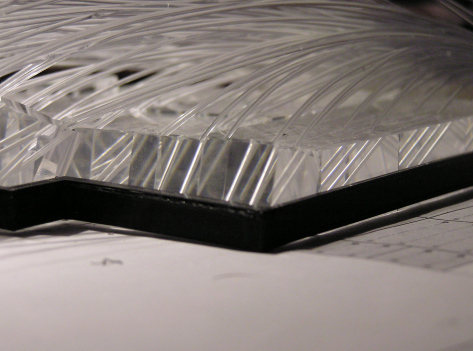
\includegraphics[width=0.6\textwidth]{ImgChap1/fibretest}
	\caption{A photograph of a fibre routing test being carried out to optimise pathing within the detector. The test utilised length of clear fibres inserted into plastic tiles.}
	\label{fibreroutingtest}
\end{figure}

\subsection{Detector Enclosure}

The enclosure that supports the detector elements is based around 4  

The base and lid of each layer of the detector is formed by a sheet of 1mm thick black carbon fibre shaped like an elongated disk with a diameter of 330mm, extended towards at the bottom of the detector, shown in Figure \ref{CarbonFibrePlate}. 

\begin{figure}
	\centering
	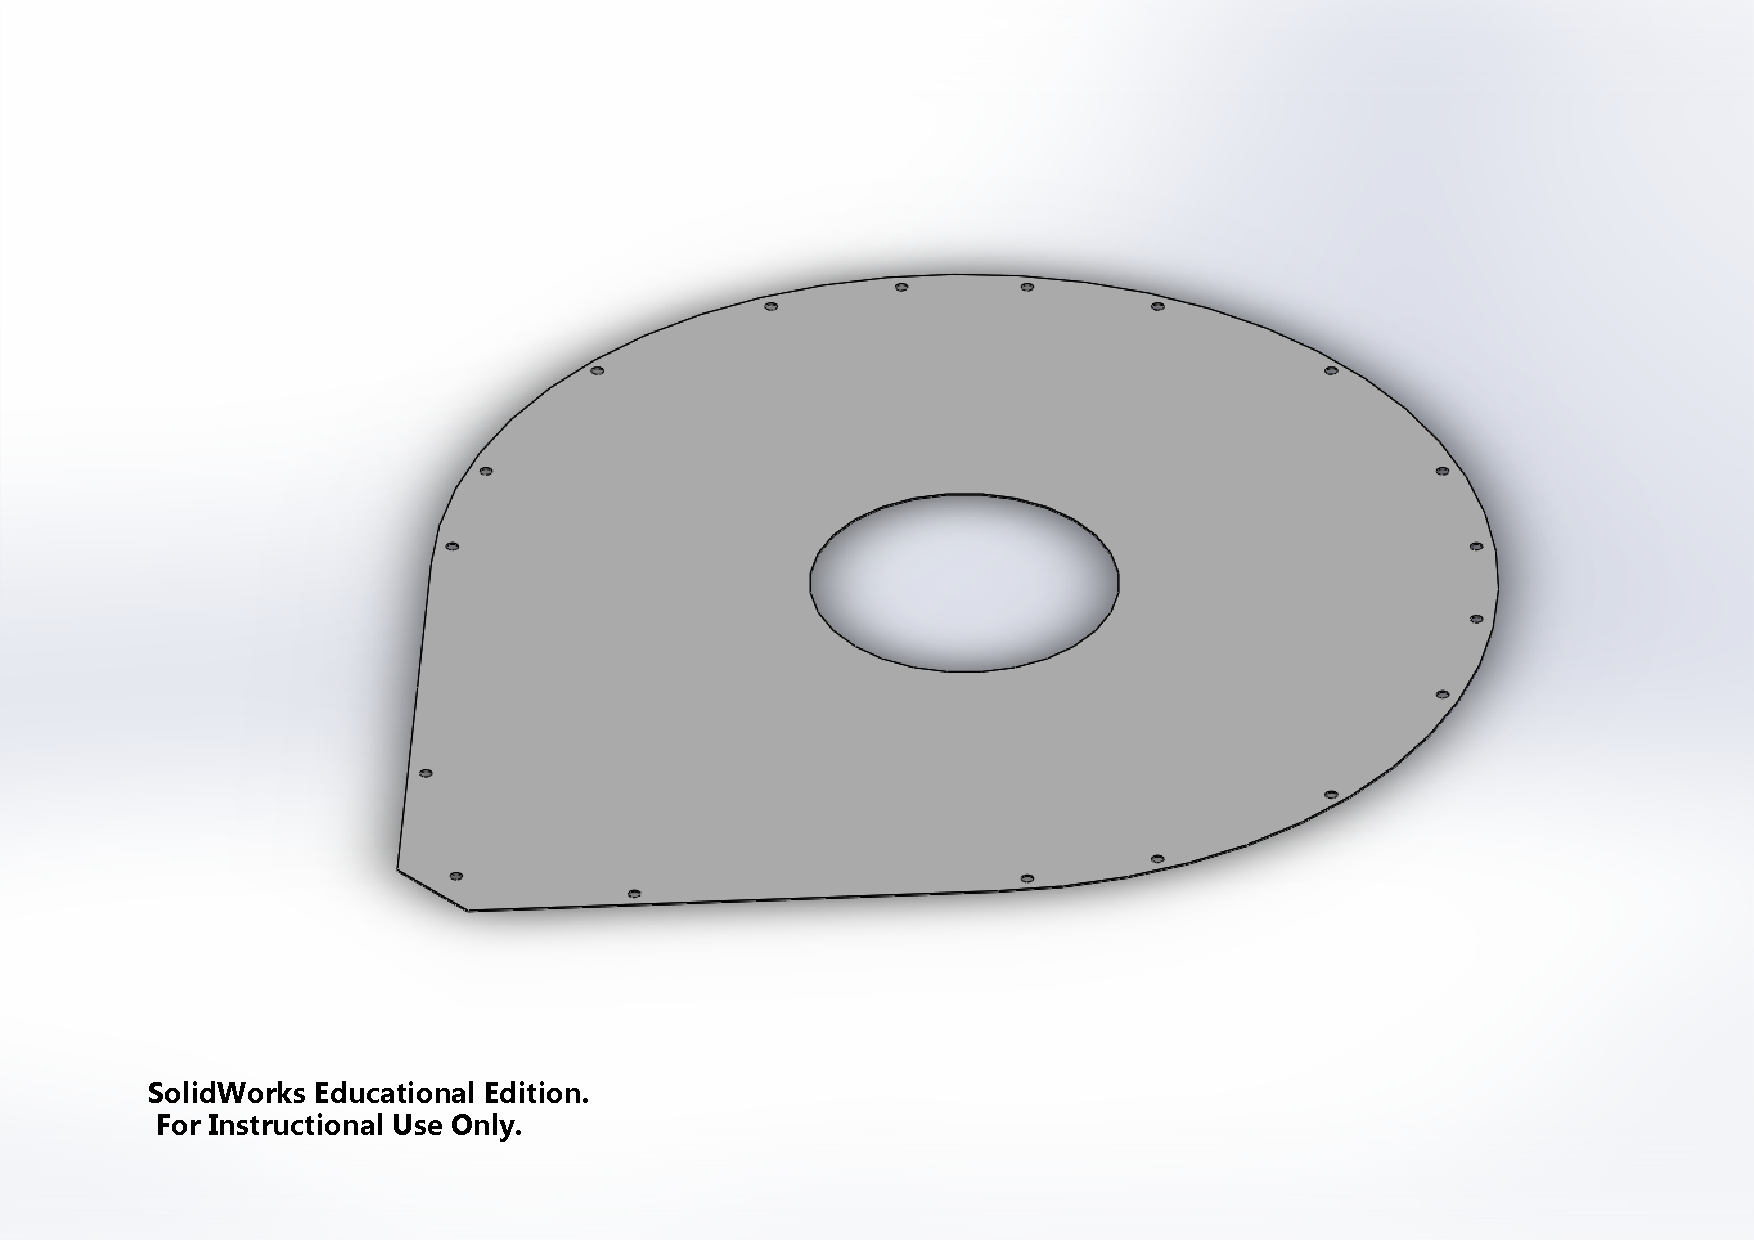
\includegraphics[width=0.6\textwidth]{ImgChap1/CarbonFiberPlateDerek}
	\caption{A CAD diagram of one of the 1mm thick carbon fibre plates used in the hodoscope. \textbf{FIX THE PICTURE}}
	\label{CarbonFibrePlate}
\end{figure}

Between the carbon plates a central \textbf{plastic} support ring and at the outer edge 13 \textbf{plastic} support pillars space the carbon fibre plates, and provide locations for countersunk screws to hold the outer and inner plates in place. Alternate holes pass directly through one layer into the layer below allowing the two layers to helm firmly together by the supporting pillars. The outer pillars are positioned and individually shaped to fill the limited gaps between detector elements and not interfere with the operation of the detector, see Figure \ref{Spacers}.

\begin{figure}
	\centering
	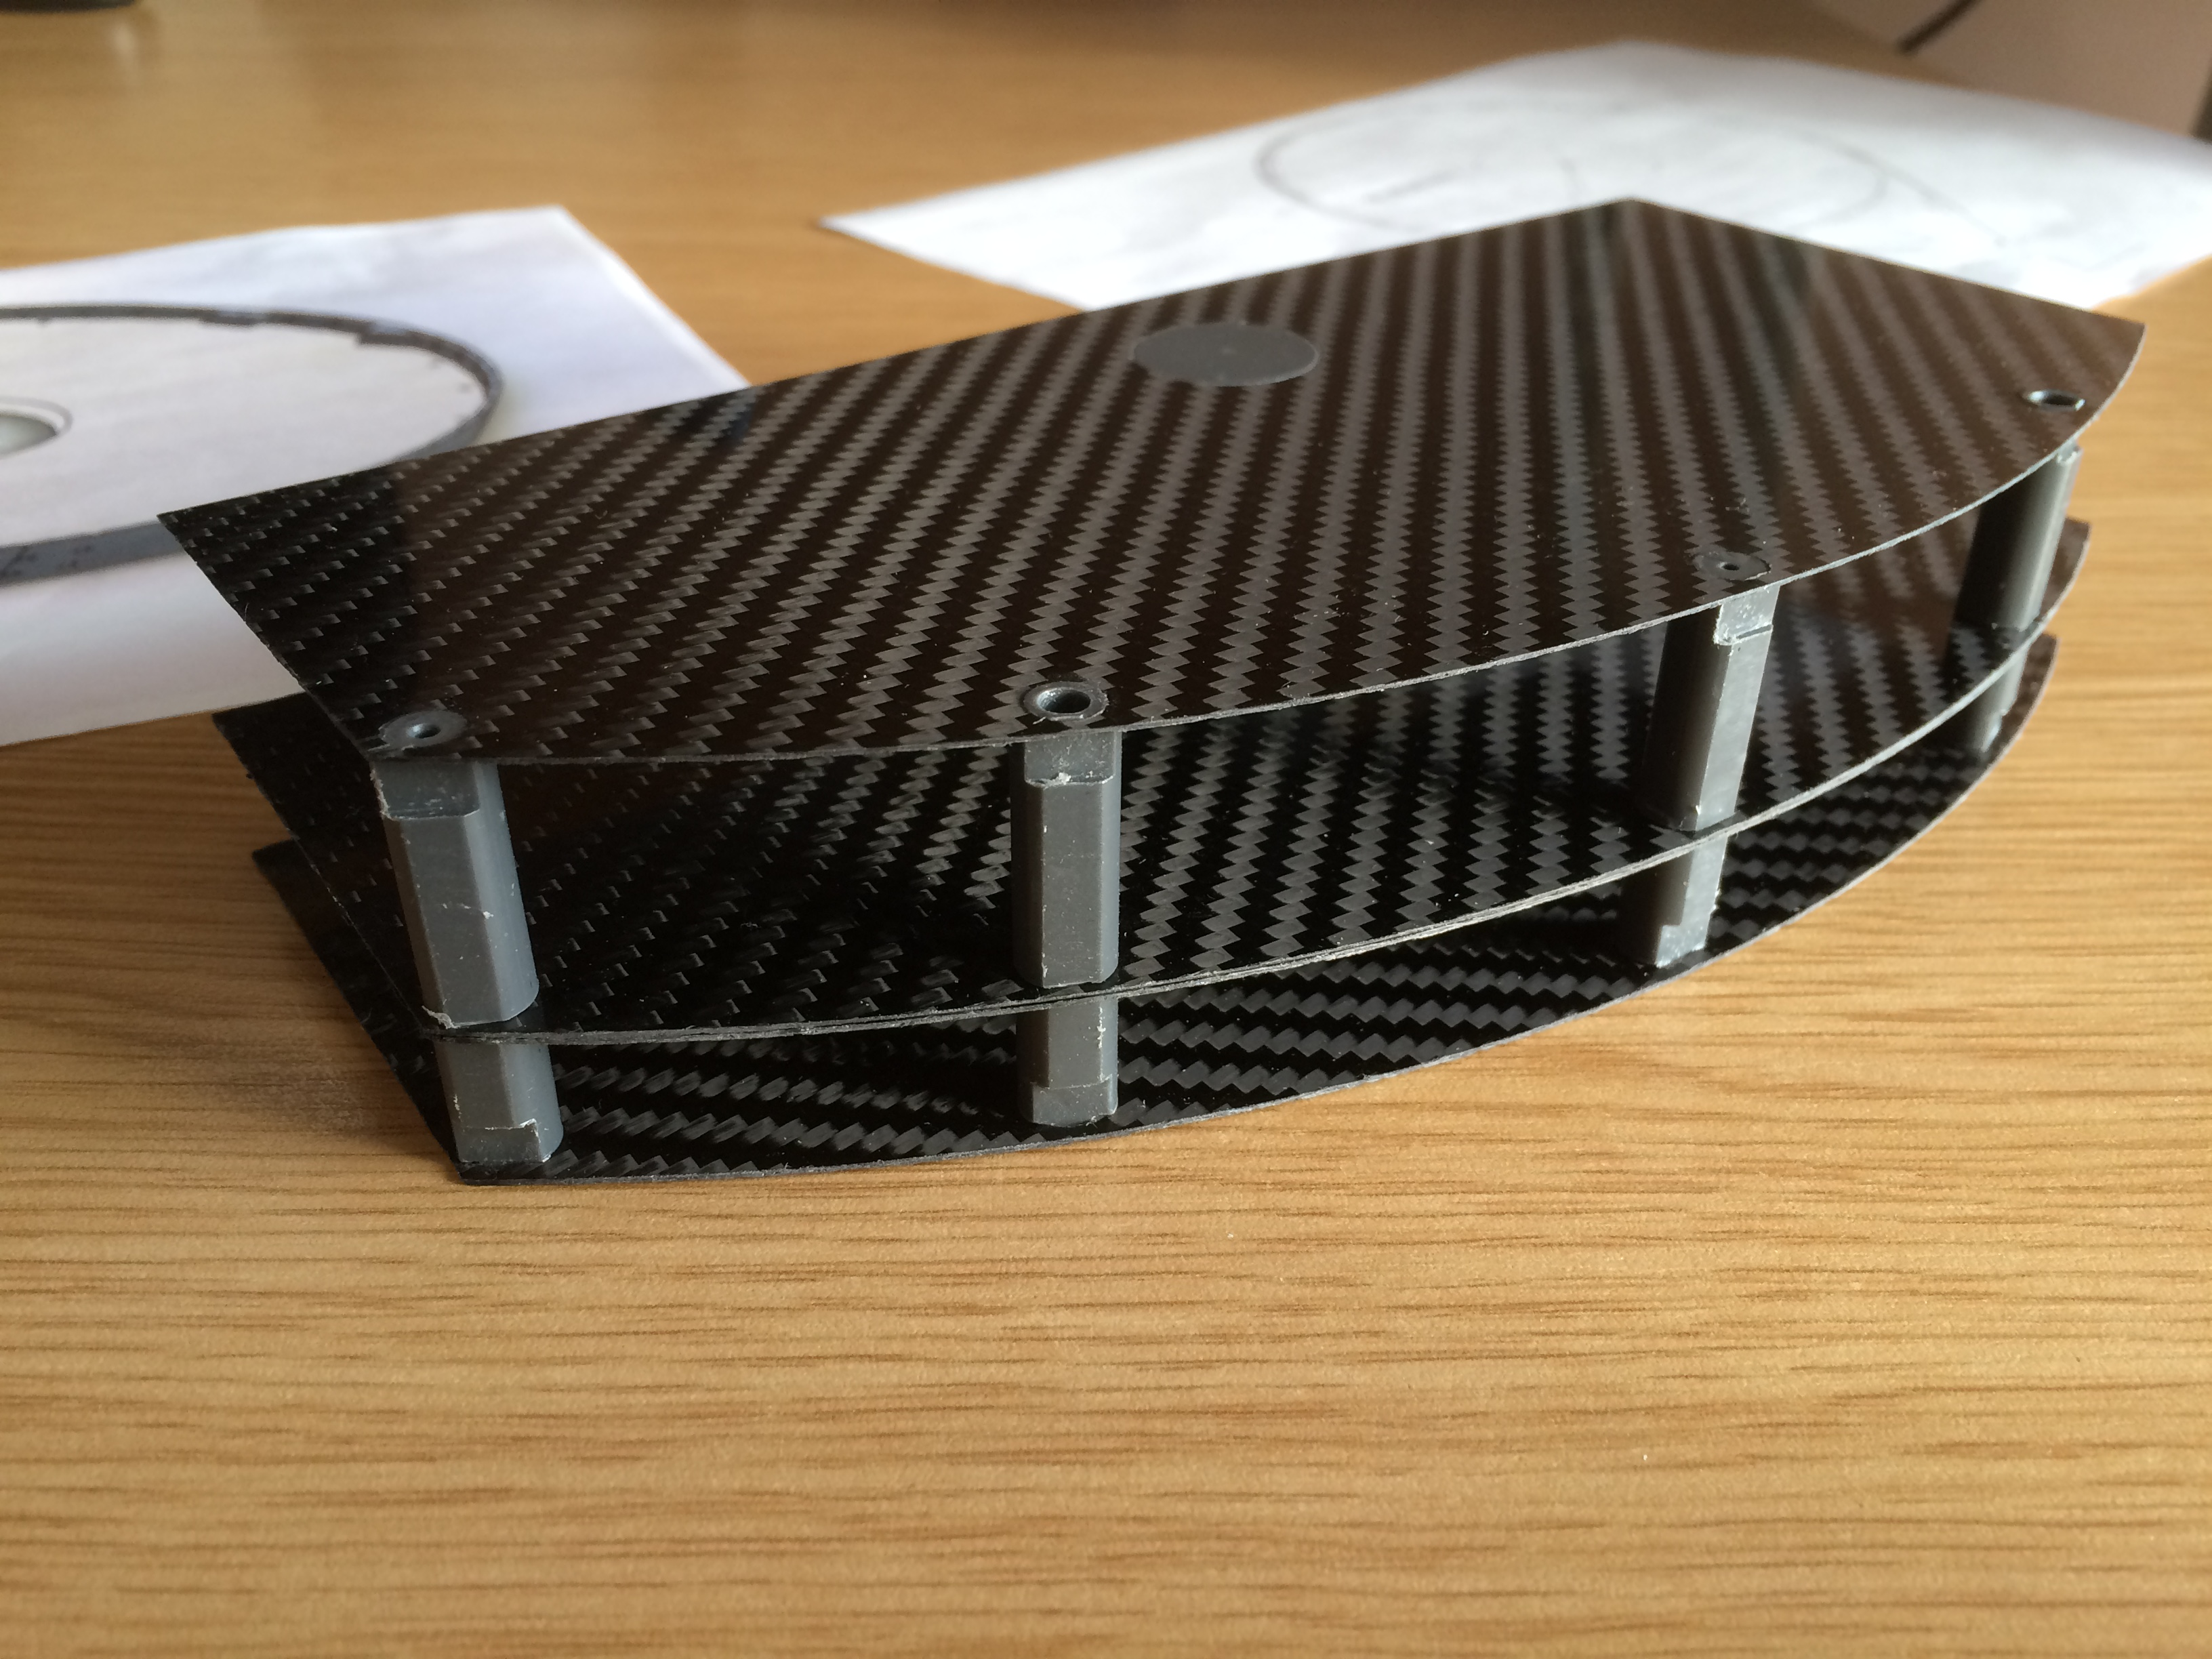
\includegraphics[width=0.6\textwidth]{ImgChap1/enclosure_hodoscope7}
	\caption{A cutaway showing a prototype of the outer spacers used to hold in place and support the carbon fibre disks in the hodoscope.}
	\label{Spacers}
\end{figure}

The fibres in the detector exit each layer through 3D printed component called the delta wing. This critical component acts to channel the fibres out of each layer of the detector, holding them in place and helping to facilitate a light tight seal for the internal components in the detector. It also acts as part of the supporting structure for the detector replacing any supporting pillars at the base of each layer. The fibres are held in place by lacing cords that thread through holes in the base of each side of the delta wing. The component is split into two interlocking pieces, one for each layer of the detector, with greater depth closer to the detector tiles for the layer of thick tiles, before transiting to provide equal square for both sets of fibres along its length. This is shown in Figure \ref{Deltawingsummary}. Just like the main body of the detector, each side of the delta wing is covered by a sheet of 1mm thick carbon fibre secured by countersunk plastic screws, sealing in the fibres it protects. 

\begin{figure}
	\centering
	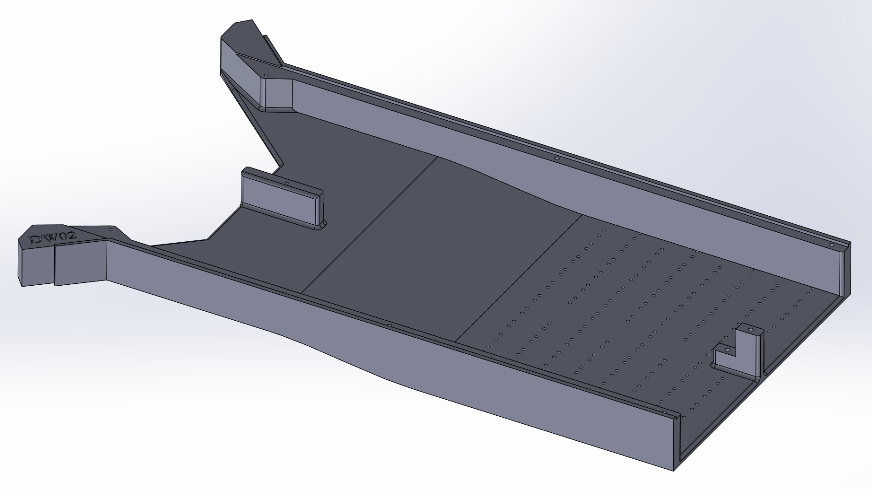
\includegraphics[width=0.6\textwidth]{ImgChap1/deltawingside}
	\caption{A CAD drawing of the hodoscope delta wing section connected to the thin layer of the detector.}
	\label{Deltawingsummary}
\end{figure}

The outer edge of the detector is a flexible plastic strip that bridges the two layers of the detector and is designed to allow the carbon fibre disks to slot seamlessly into channels that run along its length, 2 back to back in the centre and one at the top and bottom, shown in Figure \ref{OuterBelt}. It attaches to the detector system though countersunk screws that fit into the outer pillars of the detector and the delta wing at its base.

\begin{figure}
	\centering
	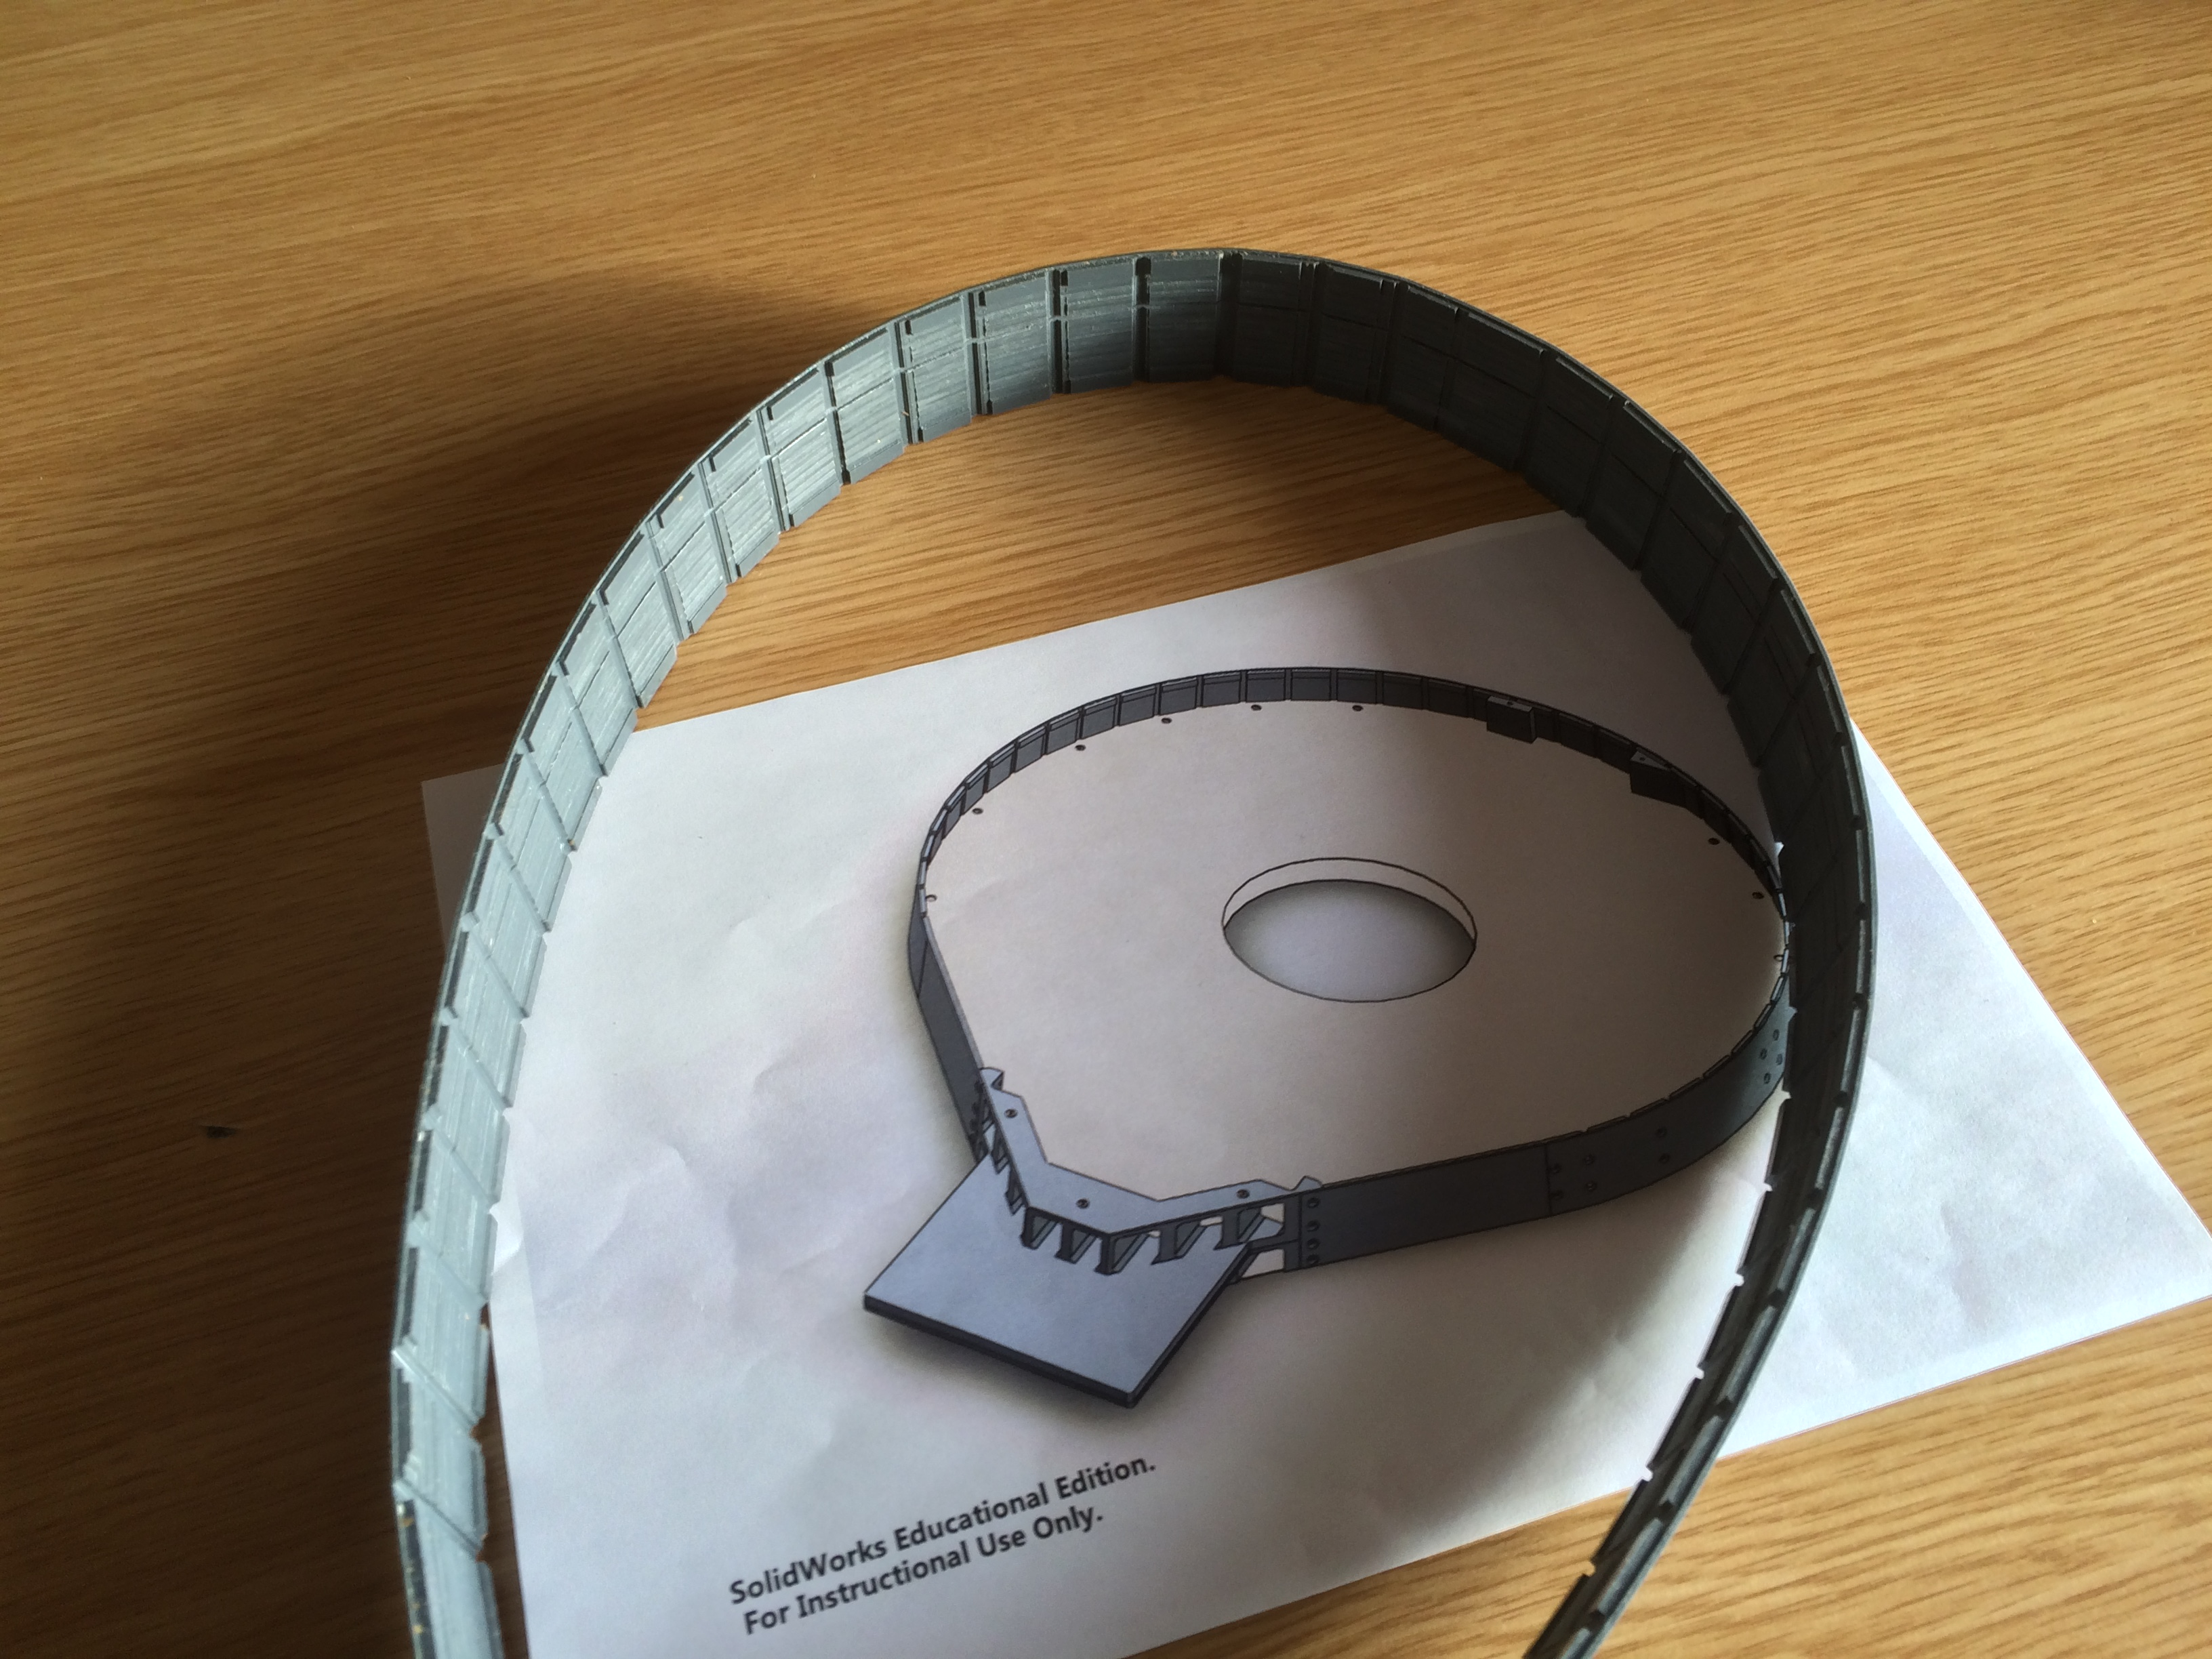
\includegraphics[width=0.6\textwidth]{ImgChap1/enclosure_hodoscope6}
	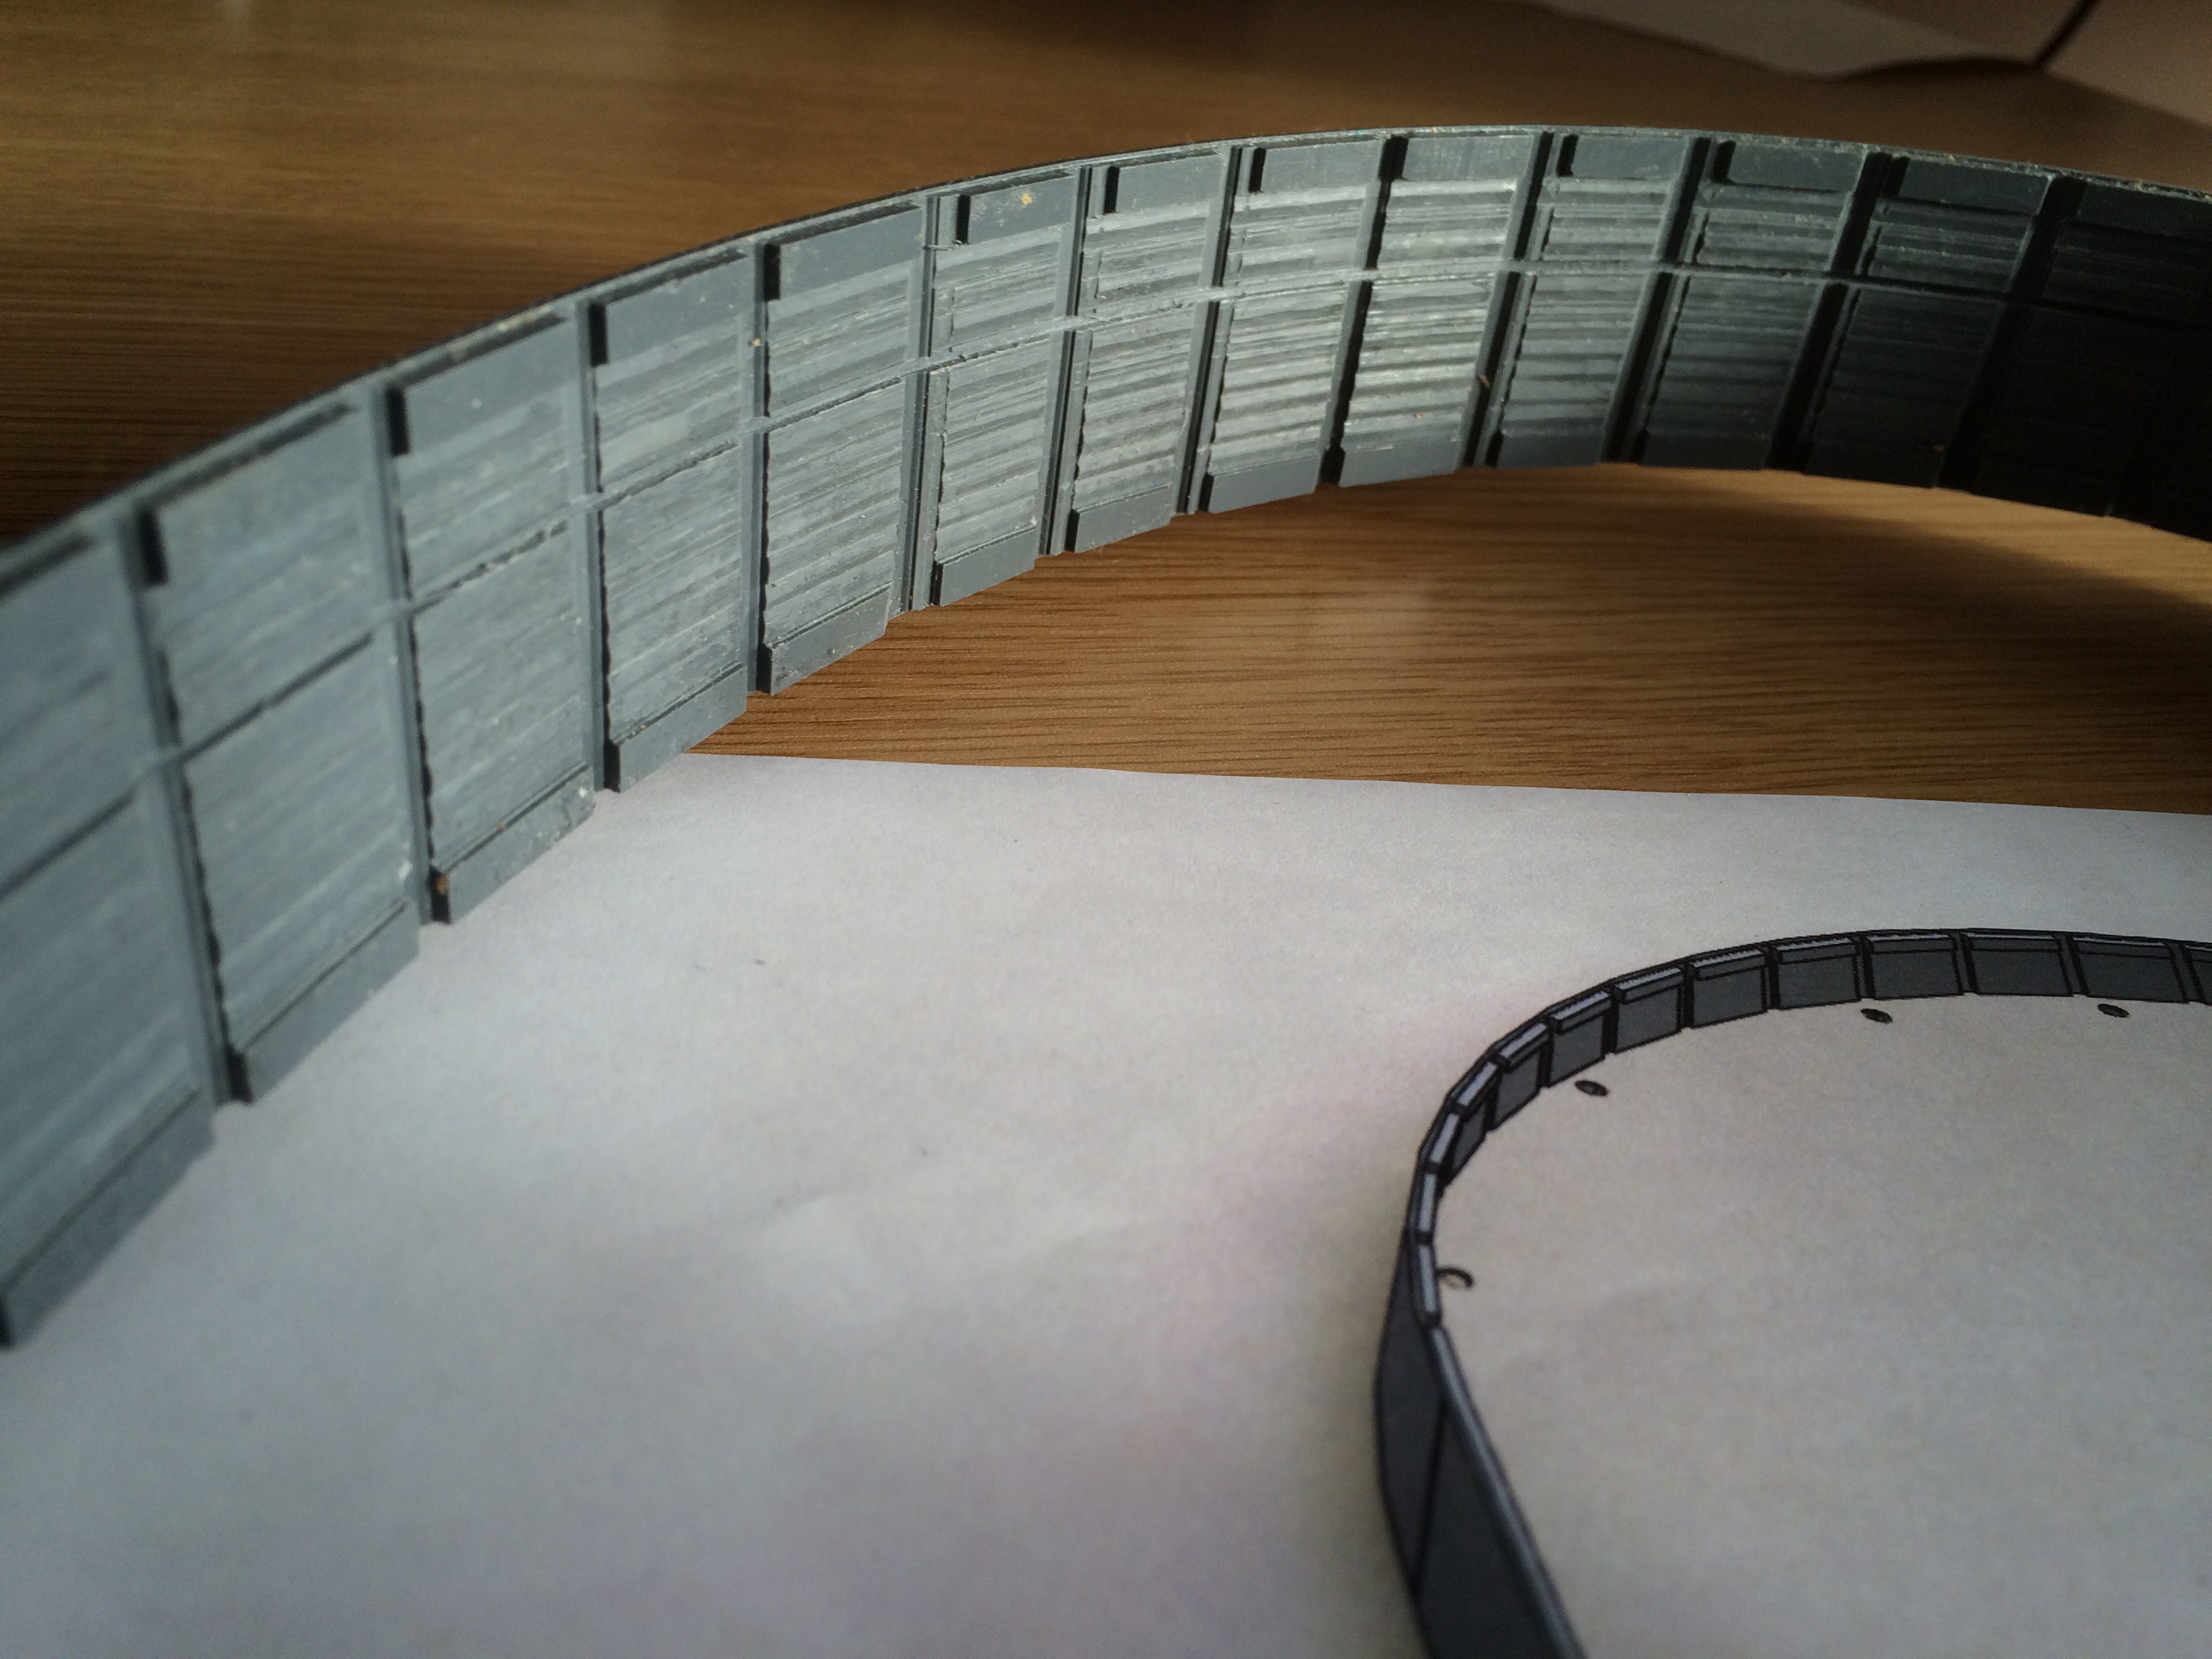
\includegraphics[width=0.6\textwidth]{ImgChap1/enclosure_hodoscope4}
	\caption{Photographs of the flexible plastic strip that forms the outer edge of the hodoscope. The channels for the outer and central carbon fibre disks can be clearly seen. }
	\label{OuterBelt}
\end{figure}

The combination of the pillars and carbon fibre sheets combine to produce a lightweight but rigid and strong construction. The Carbon fibre plates is very strong in the direction of the weave of the carbon fibre, but it is inextensible and brittle in the transverse direction. The pillars, outer rim and delta wing help to offset these issues and the interlocking design spreads any weight bearing accross the entire structure. The structure is also completely composed of materials with low atomic numbers minimising the chance of any rescattering being caused by the detector system.

In between the delta wing connector and the electronics the optical fibres are groups into bundles of 4 that are sealed from light and protected by flexible black PVC sheathing with an internal diameter of 3mm. These are grouped together and pass through CLAS in cables trays, with weight bearing tethers strategically positioned to ensure the weight of the bundles is not bourne by the fibres themselves.


\subsection{Silicon Photomultipliers}

The optical fibres juncture to the SiPMs via a 3D printed 'fishtale' connector which spreads and positions the fibres in ideal locations for optical transmission. Each connector junctions fibres to supply 8 different SiPMs, up to a maximum of 32 optical fibres. The connectors are composed from 3 interlocking pieces, a smoothly widening body, a light sealing lid and end piece into which the fibres are glued, cut and polished. The separate end pieces allow for easier insertion, repairs and replacement of fibres. A CAD drawing of this is shown in Figure \ref{FishtaleDeconstructed}.



\begin{figure}
	\centering
	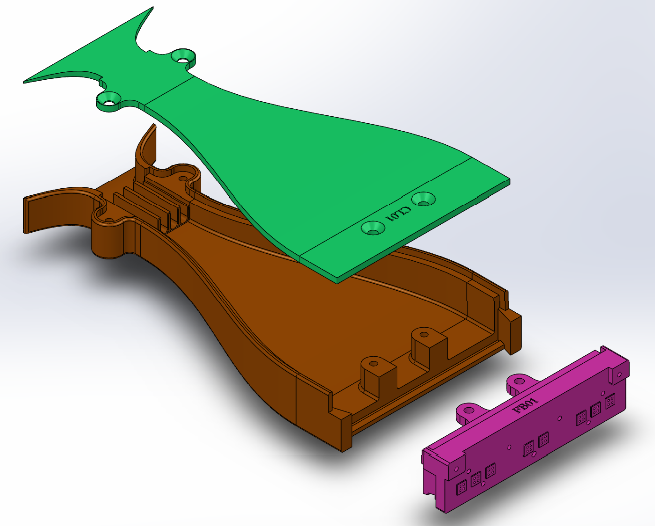
\includegraphics[width=0.5\textwidth]{ImgChap1/fishtail}
	\caption{A deconstructed 'fishtale' connector image showing the different components from which it is formed.}
	\label{FishtaleDeconstructed}
\end{figure}

The fibres from each tile are read out by an individual SiPM. These have high efficiency, high gain, fasting timing response and are sensitive enough to trigger on single photons. These properties make them well suited for a fasting timing detector such as the FT-Hodo. SiPMs are highly sensitive to input voltages requiring high voltage supplies stable to 0.01V for stable operation. However their high gain allows for beautiful clean signal separation from a high energy electron event and their main source of background, thermal noise. With a signal from a thick tile typically 20-30 times the magnitude of the background. To achieve a timing resolution $<0.5ns$ simulations indicated that at least 55 photons to produced by an event need to reach and be accepted by the SiPMs. This is one of the keys goals to surpass when optimising the detectors design and operation. 

The FT-Cal selected APDs over SiPMs because of concerns over possible radiation damage. In the hodoscope they are operating a considerable distance away from the beamline and the main concern, neutron flux, is expected to cause minimal damage over the lifetime of the detector at these distances. \cite{FTTDR2012}.

\begin{figure}
	\centering
	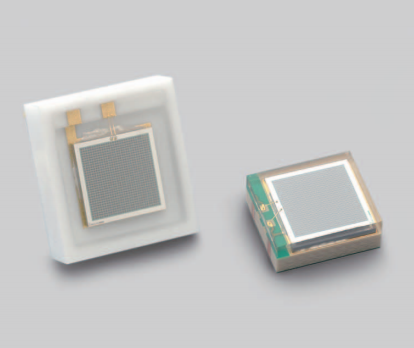
\includegraphics[width=0.5\textwidth]{ImgChap1/sipm}
	\caption{Photograph of 2 3x3mm SiPMs, the right hand model is a surface mounted version that was used in the hodoscope.}
	\label{sipm}
\end{figure}

\subsection{Electronic Boards.}

The SiPMs are mounted mezzanine boards in two groups of 8 with each group supplied by a separate high voltage connection and its own channel by channel adjustable preamplifier boards. There are 15 mezzanine boards in total providing support for the 232 channels of the hodoscope. The all fit into a VME crate along with a control board, with a single low voltage rail supplying PCBs. Through the controller the operation and temperatures of critical components on the boards can be monitored and the high voltage of individual channels adjusted. The SiPMs are gain matched into groups with similar voltage requirements, but adjusting individual channels is necessary for optimal performance. A photo of the front face of the mezzanine boards where the SiPMs are mounted is shown in Figure \ref{electronboards}.

\begin{figure}
	\centering
	\includegraphics[width=0.5\textwidth]{ImgChap1/mezzboards}
	\caption{Photograph of the front face of the mezzanine boards secured in place in the VME crate.}
	\label{electronboards}
\end{figure}

Signals from the amplifier boards are passed to Flash ADCs for processing. \textbf{NEED TO ADD MORE.}

\begin{figure}
	\centering
	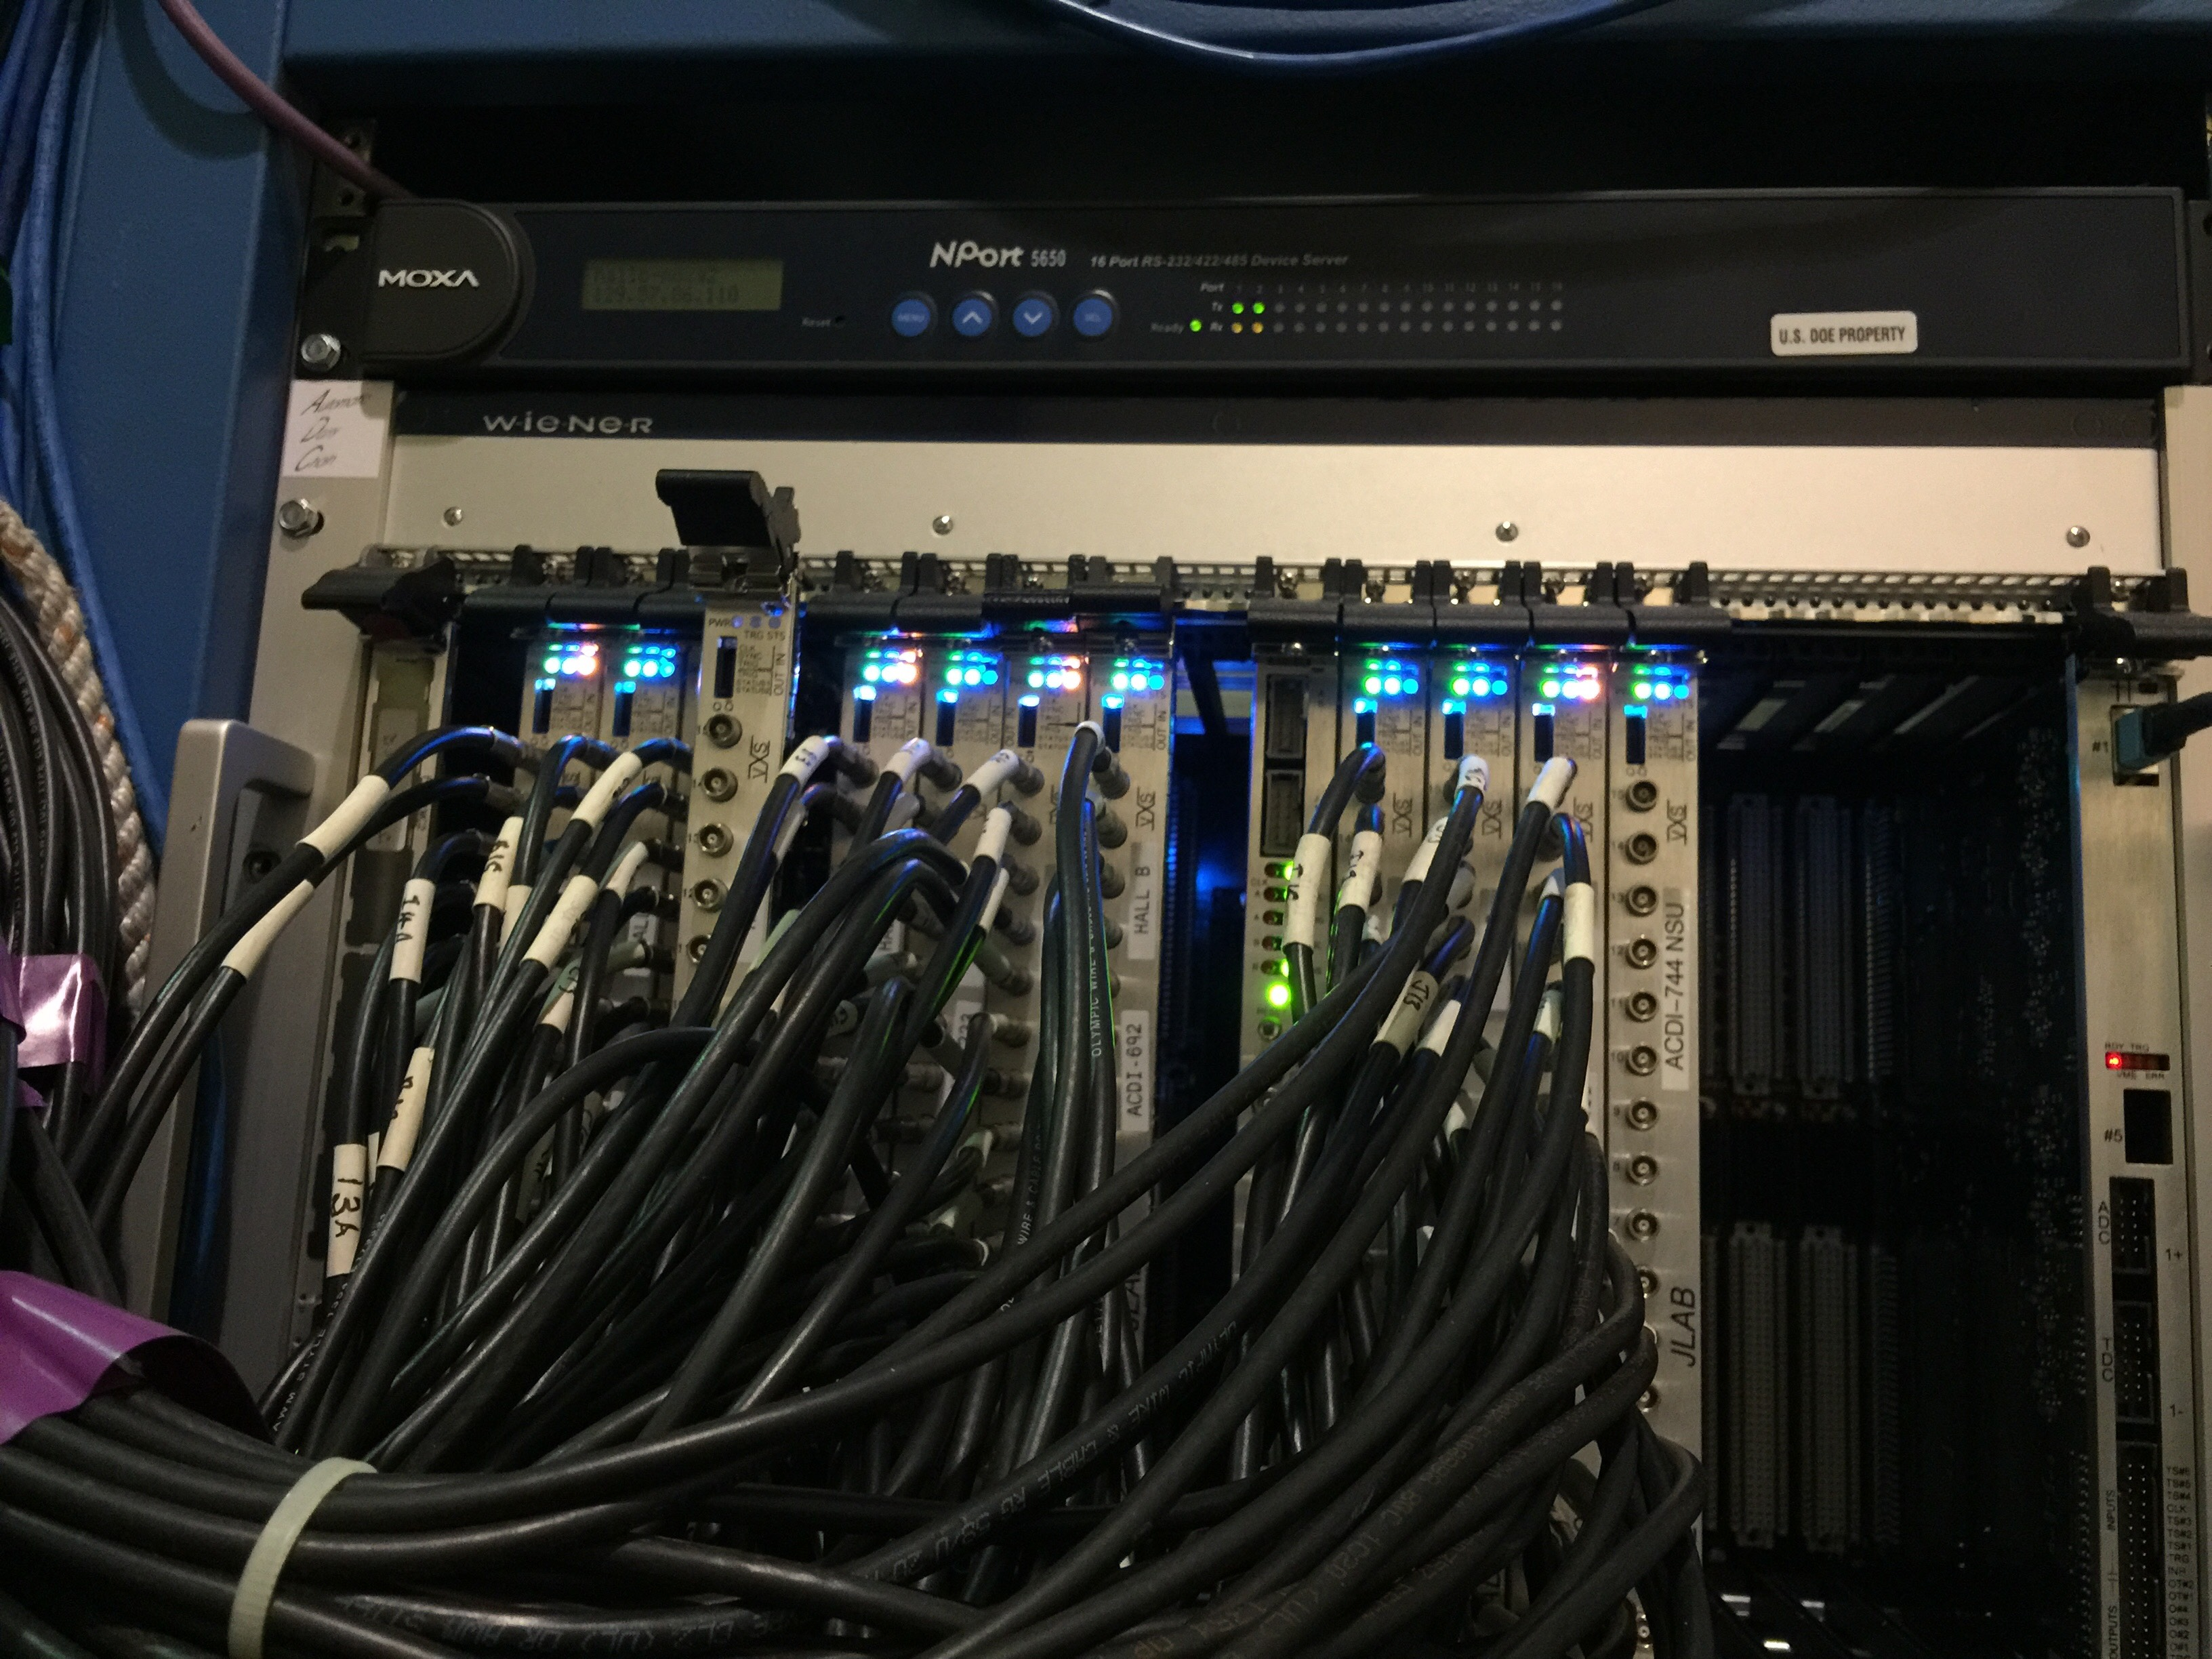
\includegraphics[width=0.5\textwidth]{ImgChap1/FlashADC}
	\caption{Photograph of some of the flashADCs used as read-out from the hodoscope during testing at Jefferson Lab.}
	\label{FlashADC}
\end{figure}

%To achieve this a highly segmented design based on fast responding plastic scintillator tiles   
%
%Describe in more detail the aims and constaints of major design decision of the hodoscope.
%
%Explain decision on choices of tiles, fibres, SiPM etc. Why not other options?
%
%Overall description of the detector



\subsection{Signal Transmission}

For optimal performance of the detector system it is critical to maximise the percentage of photons produced in the scintillators that reach the SiPMs. Improving the capture cross section and transmission of the WLS fibres is essential to this.  Compared to the volume of the scintillators the surface area of the WLS fibres is small and even if a photon enter this region there is a limited photon capture angle for transmission. To improve the chances of capture, each of the tiles is coated in 3 layers of highly reflective $TiO_{2}$ based scintillator paint with a reflectivity of $\sim 96\%$ in photon wavelength range produced by the tiles. Ensuring many passes of the photons are possible before entering the fibres. The ends of the fibres are mirrored used the same material ensure photons that were captured by the fibre but not in the transmission direction of the fibre are reflected back up the fibre towards the SiPMs. 

\begin{figure}
	\centering
	\includegraphics[width=0.5\textwidth]{ImgChap1/meson2}
	\caption{Images of the painted tiles and fibres.}
	\label{PaintedTilesandFibres}
\end{figure}


$TiO_{2}$ paint was selected for its high reflectivity, consistency and ease of application accross the 232 tiles and 784 fibres. Other candidate materials with theoretically higher reflective indices proved either inconsistent or impractical to apply to the geometry and volume of tiles and fibres.

Another critical component in the final output of light at the SiPMs is transmission of the light both within and between material boundaries. Maximising attenuation length in the materials, minimising air gaps and transitions, while keeping those that exist to occur between materials of similar refractive indices. The the quality and consistency of the application of optical cement used between the tiles and fibres, the fusion splice and the precision junction between the optical fibres and the SiPMs are all are the critical points for transmission.

\subsection{Light sealing}

A signal of great amplitude is of limited use unless outside sources of noise can be minimised. In terms of the light yield the essential componants are sealing of the detector system from outside sources of light and isolating each channel from each channel from each other to minimise crosstalk between elements. The entire detector is designed with these twin considerations in mind. 

The reflective coatings around the detector elements maximise their own transmission while simultaneously minimising possible crosstalk. Similar principles follow for the optical fibres, where bend radii are kept above minimum thresholds to increase transmission and reduce crosstalk. 

Points of intersection between different elements of the detector are such as the fishtale connector lids are designed with recesses to provide secure connections between components but also to maximise the length of light path required to pass through, forces light to reflect from multiple matt black surfaces to enter. Reducing the amount of light that passes through any gap. 

\begin{figure}
	\centering
	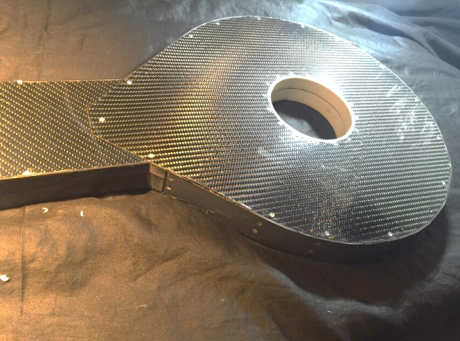
\includegraphics[width=0.7\textwidth]{ImgChap1/sealed}
	\caption{The sealed head of the detector.}		
	\label{sealedlollypop2}
\end{figure}

Most of the surfaces of the detector are made in black for both low transmission and beneficial absorptivity properties. Where possible multiple precautions are engineered into the design of components to minimise the effect of external light sources. For example when groups of fibres pass between the head of the detector and the electronics they are sealed in protective lightproof black PVC sheeting and further sealed by a surrounding layer of tedlar sheeting encompassing all the fibre bundles creating a seamless join between the delta wing of the detector and the entrance to the fishtale connectors. 

%Tedlar sealing.
%
%PVC insulation.
%
%Silicon putty.
%
%Bespoke construction.
%
%Reflective materials.

\subsection{Support structure and Shielding}

Tungsten pipe

Fibre routing through CLAS.

Moeller cone.

\subsection{2 layered design}

Not sure where it's best to insert a section about this.

Thicker layer for increase light output leading to improved timing resolution.

Thinner layer for improved background rejection.

Space limited so a balance between both layers crystal thickness is necessary. Needing to leave space for the support structure and fibres to path out of the detector.
\chapter{Simulations}

\section{Simulations}

Two GEANT4 based simulations of the hodoscope were developed in 2011 by Derek Glazier at The University of Edinburgh. The first modelled individual tile and fibre combinations in the hodoscope and the transport of photons through these to the SiPMs. Using this the dimensions, configurations and properties of the tiles and fibres could be adjusted to model and optimise the design of the system. The second simulation modelled the operation of the entire detector in conjunction with the calorimeter to determine their performance working together. Details of the results from the first simulation will be discussed in this section, with further details available in \cite{FTTDR2012}.

\begin{figure}
	\centering
	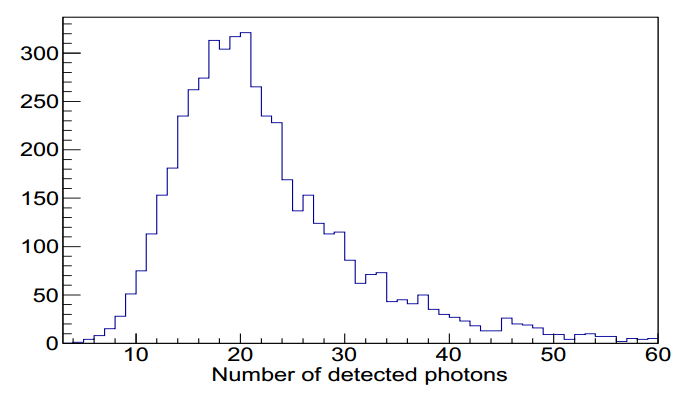
\includegraphics[width=0.9\textwidth]{ImgChap1/mip}
	\caption{Sample results from a validation simulation of the photon output of a MIP in the CLAS inner calorimeter hodoscope. The results matched well with the performance of the detector system. \cite{FTTDR2012} }
	\label{SimulationMIP}
\end{figure}

The simulation determines the energy deposited in the crystals using standard GEANT4 physics models with the properties of the components used (light output, reflectivity, refractive index, etc) inserted to realistically model the detector element design.

The valdity of the simulation was checked by using the same physics to model the CLAS inner calorimeter hodoscope. The output of which is shown in Figure \ref{SimulationMIP} for a MIP, producing a peak of $\sim$18 photoelectrons. This was in good agreement with the performance delivered by the actual detector system.


\subsection{Tile Thickness Simulations}

The amount of energy deposited in a tile by a MIP is proportional to its path length when passing through the scintillator. A thicker tile will result in more photons being released but only a proportion of these will be trapped my the optical fibres. The effect of changing the thickness of the tiles and varying both the number and diameter of optical fibres was simulated, the results of which are shown in Figure \ref{SimulationTileThickness}.


\begin{figure}
	\centering
	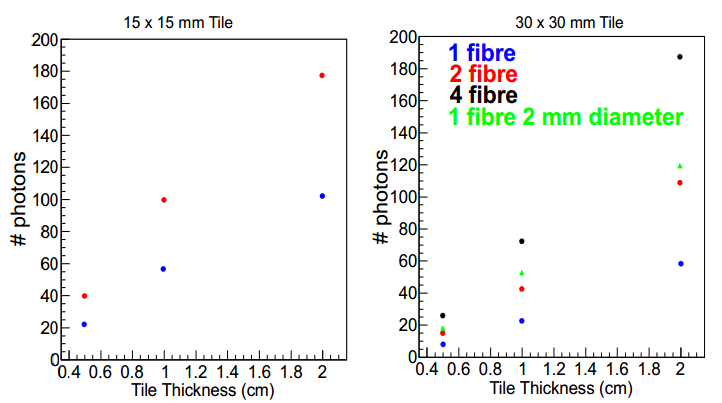
\includegraphics[width=0.9\textwidth]{ImgChap1/tilesim}
	\caption{Simulations of the variation in the photon output of detector tiles with changing thickness and different output fibre configurations. \cite{FTTDR2012}}
	\label{SimulationTileThickness}
\end{figure}

The results show a strong correlation between both increasing tile thickness and number of fibres for both 15x15 mm and 30x30 mm tiles. However there is limited space available for both scintillator and tile routing, so limits must be placed on both. The simulations showed a clear advantage of utilising four 1 mm diameter fibres over one larger 2mm diameter fibre for a 30x30 mm tile, which would occupy a similar volume within the detector.

The simulations indicate that the geometry of the P15 tiles would outperform the larger P30 tiles. A 2 fibre P15 outperforms a 4 fibre P30 at all thicknesses simulated, although the gap closes with increasing tile thickness. However 4 P15s with 2 fibres would require the space for twice as many fibres for the same coverage as 1 P30 with 4 fibres. In addition the smaller tiles would result in a lower acceptance for the detector, with addition space required for reflective materials and unavoidable air gaps between the scintillators. A compromise utilising both designs was selected with a band of P15 tiles surrounding the regions of highest flux at the centre of the detector with the majority of the acceptance covered by the larger P30 tiles. A summary of the simulation results for the performance of the selected thicknesses of the two layers of the detector are shown in Table \ref{SimulationTileThickSummary}.

\begin{table}\centering
	\renewcommand{\arraystretch}{1.3}
	\begin{tabular}{ @{}l  c  c@{}} 
		\toprule
		Tile Type & Thickness & Expected Photons \\
		& {\small [mm]}& \\
		\midrule
		P15 & 7 & 70 \\
		& 15 & 150 \\
		\midrule
		P30 & 7 & 55  \\
		& 15 & 120 \\
		\bottomrule
	\end{tabular}
	\caption{Summary of the expected photon output of the detector tile dimensions selected for use in the hodoscope.}
	\label{SimulationTileThickSummary}
\end{table}

\subsection{Timing Resolution}

Following a similar format to the results for tile thickness, the results for timing resolution are shown in Figure \ref{SimulationTiming}.

\begin{figure}
	\centering
	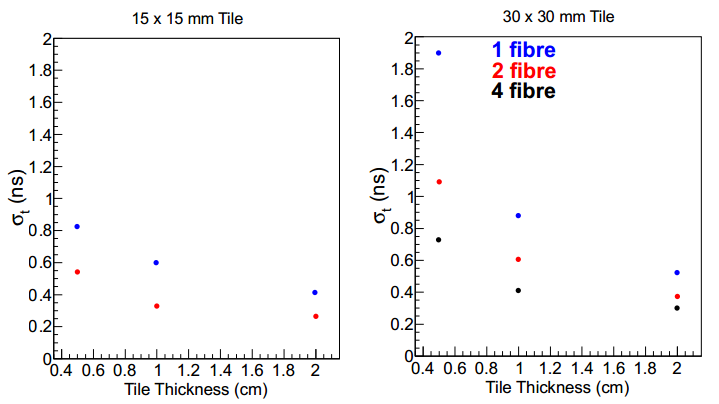
\includegraphics[width=0.9\textwidth]{ImgChap1/timingsim}
	\caption{Results showing how the timing resolution of detector elements varies with thickness and different output fibre combinations. \cite{FTTDR2012}}
	\label{SimulationTiming}
\end{figure}

The critical point to notice is that increasing the number of photons collected improves the timing resolution of the detector elements. The absolute rate of improvement is most significant at lower levels of photon collection, but the effects continues throughout the range of thickness tested in these simulations. The results indicated that sub nanosecond timing resolution is achievable for the detector element design and 0.5 ps levels of timing could be achieved with photon output levels of $\sim$55 photoelectrons. A summary of results for the tiles dimensions used in the construction of the detector are shown in Table \ref{SimulationTileTimingSummary}.

\begin{table}\centering
	\renewcommand{\arraystretch}{1.3}
	\begin{tabular}{ @{}l  c  c  c@{}} 
		\toprule
		Tile Type & Thickness & Expected Photons & Timing Resolution \\
		& {\small [mm]}& & {\small [ns]}\\
		\midrule
		P15 & 7 & 70 & 0.40\\
		& 15 & 150 & 0.30\\
		\midrule
		P30 & 7 & 55 & 0.50\\
		& 15 & 120 & 0.35\\
		\bottomrule
	\end{tabular}
	\caption{Summary of the expected timing resolution of the detector tile dimensions selected for use in the hodoscope.}
	\label{SimulationTileTimingSummary}
\end{table}

\subsection{Fibre Bending}

Light losses due to the bend radius of fibres both within the hodoscope enclosure and while routing through CLAS were also simulated as part of these tests, the results of which are shown in Figure \ref{SimulationBendRadius}. The results matched closely by the results reported by Kuraray to limit the bend radius to no less than 2cm, ideally higher to minimize light losses during transport. 

\begin{figure}
	\centering
	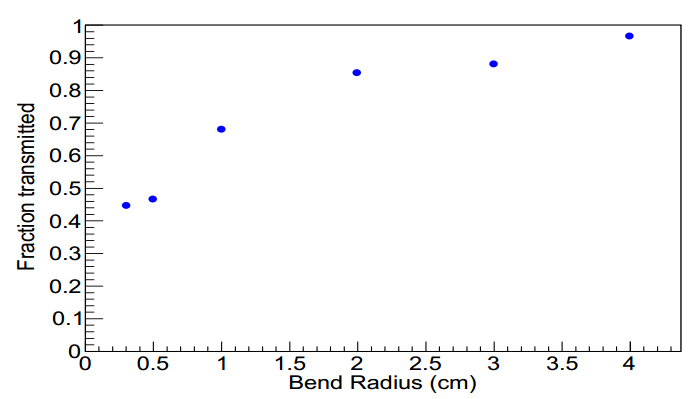
\includegraphics[width=0.9\textwidth]{ImgChap1/bendsim}
	\caption{Results of a simulation measuring the fraction of light loss in a wavelength shifting fibres at different bend radii. \cite{FTTDR2012}}
	\label{SimulationBendRadius}
\end{figure}

\subsection{Radiation Dose}

In addition to the light transport simulations a further study to determine the radiation exposure of the hodoscope was carried out by INFN Genoa. Determining the dose that different elements of the hodoscope would be exposed to ensured they could be suitably resistant and their performance would not degrade significantly over the lifetime of the detector. 
The simulations indicated that without the M\o{}ller shield in place, the largest does would be incurred by the inner pixels of the detector at a rate of 3.8 rad/h. Figure \ref{SimulationRadDose} shows a plot from the INFN simulation, with each pixel representing one of the, 15x15 mm tiles in the calorimeter that is positioned directly behind the hodoscope. 

\begin{figure}
	\centering
	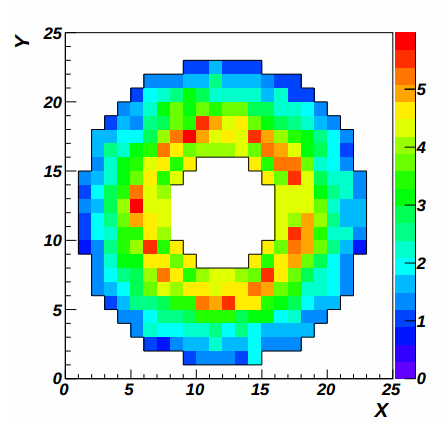
\includegraphics[width=0.9\textwidth]{ImgChap1/raddose}
	\caption{Results from a simulation of the radiation dose experience by the FT-Cal crystals in rad/h at $10^{35}cm^{-2}s^{-1}$ luminosity. Maximum values of just over 5 rad/h were obtained for some of the inner crystals, although averaged over each crystal in the hodoscope this represents a peak of 3.8 rad/h. \cite{FTTDR2012}}
	\label{SimulationRadDose}
\end{figure}

Taking the peak element value of 3.8 rad/h and considering this to be the dose for all elements accross the hodoscope, produces an annual does of 33 krad for each crystal. A large number of studies have shown that exposure to radiation can change the properties of plastic scintillators; reducing the light yield and therefore timing resolution of the tiles. Similar effects have been shown to occur in wavelength shifting fibres and optical cements, reducing their transparency and increasing attenuation length, lowering the performance of the materials.

\textbf{Write a paragraph about literature studies on them, generally done at much higher radiation doses and typically imparted over a much shorter period of time. Studies on the materials used have shown them to be radiation hard to well beyond the expected levels of radiation and much of the damage is expected to be counteracted by annealing processes.}



%Geant4 based simulations were carried out to optimise the design of the detector system. In particular the design of the detector elements was studied as this was the first time such a design had been used before. Keep this short as I wasn't involved in developing, just using this element of the project.

\cite{golovko2008use}


\chapter{Beamtime}

\section{Beamtime}

Throughout the development of the hodoscope many different experiments have been carried out in the lab to gather more data on the performance of the different elements of the hodoscope. Most of these were carried out using radioactive sources or collected data using cosmic rays. Both of these sources are readily available but are either limited by the energy of the source or the rate of the cosmics. To truly test the detectors performance in an environment comparable to which it will be used once installed requires beamtime. There have been 3 beamtests throughout the detectors development, the first carried out at Jefferson Lab and the following two at the Double Annular $\Phi$  Factory for Nice Experiments (DAFNE or DA$\Phi$NE) Beam Test Facility (BTF). Each one was done in conjunction with a prototype of the FT-Cal, simulating their operating environment in CLAS12.

\subsection{First Test: Hall B at JLAB}

The first test used only a single 15 x 15 x 10 mm$^{3}$ tile read out by 2 wavelength shifting fibres. These were set into channels cut into the surface of the tile, rather than inset into holes. The test configuration in Hall B at JLAB is shown in Figure \ref{HallBTestSetup}

\begin{figure}
	\centering
	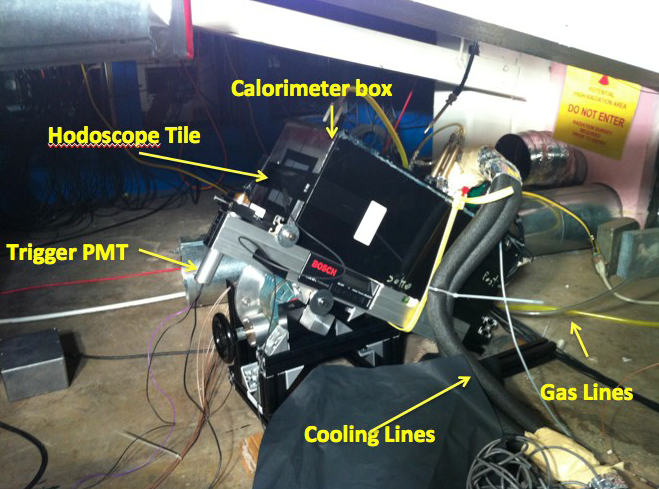
\includegraphics[width=0.7\textwidth]{ImgChap1/firsttest}
	\caption{The set-up for the first beamtest in Hall B.}
	\label{HallBTestSetup}
\end{figure}

The main aim was to provide an initial proof of principle test of the equipment and to provide further information to guide the development of the detector system under beam conditions. The single hodoscope tile was positioned in front of one of the elements of the calorimeter to take coincidence measurements.

The results of the energy deposited in the hodoscope and calorimeter tile can be plotted in 2D to determine the spread of hits measured in the test. An example is shown in Figure \ref{HallBTestResult}, with a clear region of coincident hits measured between the two detector tiles. 

\begin{figure}
	\centering
	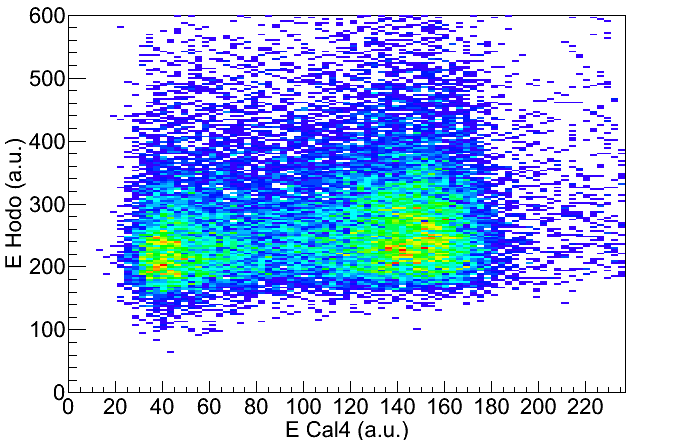
\includegraphics[width=0.9\textwidth]{ImgChap1/HodoTest2}
	\caption{An example of the spread of Energy deposited in the test set-up in Hall B. The energy of hits in the hodoscope vs the calorimeter are shown (terms of the ADC channel). The cluster on the left represents pedestal measurements and the cluster on the right are coincident hits between the two detectors.}
	\label{HallBTestResult}
\end{figure}

This initial test of a simple readout situation was a success and provided plentiful information to improve the design of the detector system. However the light output and isolation of the tiles needed to be improved to reach the design requirement of the system.


\subsection{Second Test: BTF at DA$\Phi$NE}

This following set of beam tests took place at the DA$\Phi$NE $e^{+}e^{-}$ collider siutated at the INFN Frascati National Laboratory, Frascati Italy. This facility primary collides electrons and positrons at a centre of mass energy of 1.02 GeV to produce $\phi$ mesons that primary decay to kaons that are the main focus of the experiments taking place at the accelerator. The leptons are in the facility are first accelerated by a LINAC to 510 MeV before being injected into the accumulator. However when injection is not taking place the beamline can be delivered to a beam test area (BTF). \cite{mazzitelli2003commissioning}. The BTF facility is capable of delivering beam for a wide range of energies and multiplicities and is mainly used for calibration experiments.


\begin{figure}
	\centering
	\includegraphics[width=0.7\textwidth]{ImgChap1/BTF}
	\caption{An arial overview of the accelerator facility at DA$\Phi$NE. \cite{mazzitelli2003commissioning}}
	\label{BTF}
\end{figure}

The tests main purpose was to test a range of hodoscope elements at the same time, in coincidence with multiple calorimeter elements. A total of 8 tiles were prepared 4 larger P30 tiles and 4 smaller p15 tiles, with an even split between thick (15mm) and thin (7mm) tiles. The elements prepared used initial designs for reflective materials, optical connections and electronics with 8 hodoscope channels being read out simultaneously.

\begin{figure}
	\centering
	\includegraphics[width=0.7\textwidth]{ImgChap1/frascatitile}
	\caption{Some of the tiles used during the frascati tests. 2 after being wrapped and 2 before.}
	\label{Frascati2Tiles}
\end{figure}

The Tiles used were positioned in 2 layers, with 2 wider p30s and 2 smaller p15 tiles used in each layer,  with the thicker tiles mounted behind the thinner layer. Each tile was aligned with corresponding elements in the prototype calorimeter for coincidence measurements during the experiment. For ease of readout some fibres were connected using shorter ($\sim$ 0.2m) and other longer ($\sim$ 1m) fibres. A simple diagram of the set-up is shown in Figure \ref{Frascati2SetupDiagram}. 

\begin{figure}
	\centering
	\includegraphics[width=0.7\textwidth]{ImgChap1/frascati1}
	\caption{Schematic set-up for the BTF tile tests. Configuration with the beamline directed into the page with the calorimeter positioned downstream of the prototype hodoscope.}
	\label{Frascati2SetupDiagram}
\end{figure}

The results of the tests were positive successfully taking data from the 8 tiles simultaneously in coincidence with the calorimeter. However there were clear problems with both the overall output of the tiles and the consistency of results between them, an example of these is shown in Figure \ref{Frascati2Results1}. 

\begin{figure}
	\centering
	\includegraphics[width=0.9\textwidth]{ImgChap1/frascatiresults1}
	\includegraphics[width=0.9\textwidth]{ImgChap1/frascatiresults2}
	\caption{Sample results from the first tests run at the BTF (x-axis units are photoelectrons). Results are shown for the 4 thin tiles (Top four frames)} and the 4 thick tiles (Bottom four frames). Results for both single and double electron bunches can be clearly seen, most obviously for the P30 Thick tiles. 
	\label{Frascati2Results1}
\end{figure}

The results obtained are well below the expectations from simulations, however during the tests it was found that some of the tiles experienced both poor and inconsistent optical connections both Tile$\rightarrow$Fibre and Fibre$\rightarrow$SiPM. Attempts were made to adjust these during the tests but more fundamental adjustments to the design were required to resolve some of these problems. The strongest performing tiles were the P30 thick tiles, which averaged $\sim$18 photoelectrons for a MIP. 




\begin{figure}
	\centering
	\includegraphics[width=0.7\textwidth]{ImgChap1/holderboard}
	\caption{A photograph of 8 fibre channels attached to a prototype board supporting the SiPMs.}
	\label{Frascati2SetupDiagram}
\end{figure}




\subsection{Third Test: BTF at DA$\Phi$NE}

A second set of beam studies at DA$\Phi$NE was carried out on prototype hodoscope detector in November 2012. This set of tests used a similar configuration to those utilised at the previous test, but the focus was put onto improving the optical output of the tiles demonstrating the viability of the detector design. A variety of new tiles were tested, including some previously trialled at the previous round of testing. Improvements were made to the reflective wrapping of the tiles and optical isolation of the elements. However the most significant progress was made in the quality of the optical connections tiles-fibres and fibres-SiPMs. Where each group of fibres was glued into a SiPM connector, before being polished using a series of refining grades of optical sandpaper, to ensure a clean optical connection to the SiPMs.

%Tiles used in each round of testing were positioned in 2 layers, with 2 wider p30s and 2 smaller p15 tiles used in each layer. The electronics were positioned to one side of the detector system, outside of the beamline, which necessitated the fibres from some tiles to be longer than others, see Figure \ref{Frascati2SetupDiagram}. 

\begin{figure}
	\centering
	\includegraphics[width=0.7\textwidth]{ImgChap1/frascatiphoto}
	\caption{Photograph of the prototype configuration in situ in frascati, prior to the start of the beamtime.}
	\label{Frascati2SetupPhoto}
\end{figure}

\begin{table}\centering
	\renewcommand{\arraystretch}{1.3}
	\begin{tabular}{ @{}l  c  c  c  c@{}} 
		\toprule
		Tile & Thickness &Fibre Length & Source & Photons \\
		& {\small [mm]}& {\small [m]} & & \\
		\midrule
		P30Thn & 7 & 0.2 & Eljen* & 37 \\
		P30Thn & 7 & 1.0 & Eljen* & 28 \\
		P15Thn & 7 & 0.2 & Eljen* & 23 \\
		P15Thn & 7 & 1.0 & Elgen* & 19 \\
		P30Thk & 15 & 0.2 & NE & 78 \\
		P30Thk & 15 & 1.0 & NE & 35 \\
		P15Thk & 15 & 0.2 & Eljen & 29 \\
		P15Thk & 15 & 1.0 & Eljen & 23 \\
		P30Thk & 15 & 0.2 & Elgen & 46 \\
		\bottomrule
	\end{tabular}
	\caption{Summary of tile performance during the second set of tests at BTF. Tiles marked with a * were also tested at the previous beamtime at BTF, but now with upgraded fibre$\rightarrow$SiPM connections.}
	\label{Frascati2ResultsTable}
\end{table}

Nine different tiles were tested during the beamtime, with the P30Thk tiles being switched between runs. The overall performance of the tiles increased significantly from the results obtained at the previous test, with the best performing tile peaking at just under 80 photoelectrons, shown in Figure \ref{Frascati2Results} However the results were still not consistent across size, thickness and fibre length and the majority of tiles were still performing below the potential indicated by simulations. This set of results was promising and demonstrated the tiles can reach the level of output required for suitable timing resolution of the detector. Further studies were needed to raise the number of photons reaching the SiPMs and improve the consistency of tile performance to allow every detector element to reach the same peak performance. Figure \ref{Frascati2Results} show of plot of the best performing tile in the tests.

\begin{figure}
	\centering
	\includegraphics[width=0.7\textwidth]{ImgChap1/frascati2results}
	\caption{A plot of the strongest performning tile from the second set of tests at BTF. The MIP landau is well seperated from the thermal noise across almost the full range of the ADC, peaking at an energy equivalent to just below 80 photoelectrons.}
	\label{Frascati2Results}
\end{figure}   
\chapter{Construction}

\section{Contruction}

The hodoscope was constructed in a purpose built environment in a re-purposed laboratory at The University of Edinburgh. The space was designed to minimize dust levels, exposure to UV light and provide a temperature controlled environment. The tent was constructed to isolate the detector elements for construction and fitted with an air filtration system, and specialist UV lighting that blocked out wavelengths shorter than the red part of the visible spectrum.

\begin{figure}[!ht]
	\centering
	\includegraphics[width=0.7\textwidth]{ImgChap1/NoUV_setup1}
	\caption{A photograph of the laboratory used for the construction of the hodoscope.}
	\label{HodoTent}
\end{figure}


\subsection{Tile and Fibre Preparation}

A rigorous and meticulous approach to preparing each of the individual tiles and fibres was critical to the absolute performance and consistency accross the many different channels of the detector. Initial testing was of the tiles and fibres was carried out on a small sample of the larger order supplied before the major order that allowed the preparation process to be optimised.

\subsubsection*{Tile Preparation}

The plastic scintillator tiles were cut  to size and polished by the supplier before being outsourced to a specialist firm to drill the channels for the wavelength shifting fibres. All the tiles dimensions were measured and each carefully inspected for signs of crazing or any other damage with any damaged tiles excluded from use in the detector. This data was stored for future use in optimising the arrangement of the tiles in the detector. Initially a subset of these tiles were prepared to check the quality and consistency of the scintillator tiles, ensuring the performance of the detector. Once these checks were passed each tile was hand painted with 3 thin coats of Ti$O_{2}$ reflective paint. Brushing from the centre of each side towards the edge to minimise edge lapping. After painting each side was lightly sanded to produce a smooth finish. The width of the coat of paint was then measured at multiple points using vernier callipers, comparing to the tile dimensions previously collected. This is to ensure a thickness of 0.15-0.2mm for optimal reflective properties, without excessively increasing the dimensions of each tile. This process was repeated for every side of each tile and final dimensions collated for positioning optimisation. Where corrections were needed the painted sides were first smoothed with a layer of P1200 grade sand paper before refining the surface with $3\mu$m grade optical lapping film until smooth.

Small variations across a number of successive tiles can sum up to produced significant asymmetries and misalignments across the detector volume, hence the need for such meticulous control over this process. Figure \ref{elementgap} demonstrates the inherent gaps present within tiles, minimising these is critical to maintain the alignment and acceptance of the detector system.

\begin{figure}[!ht]
	\centering
	\includegraphics[width=0.7\textwidth]{ImgChap1/gap}
	\caption{Illustration of the inherent gaps present between tiles.}
	\label{elementgap}
\end{figure}

\subsubsection*{Fibre Preparation}

Once testing was successfully completed the major batch of clear and wavelength shifting fibres was shipped to Fermi Lab to be cut and prepared for fusion splicing. Each length of fibre was checked for any signs of damage before lengths of 6m of clear fibre were and 10cm lengths of WLSF were polished using the Ice Polishing method \cite{gallas1998polishing}, before being fusion spliced together with the join protected by a protective jacket. The 1 mm diameter fibres were then put into groups of 4 and slid into protective 3mm diameter black PVC sleeving which acts to protect the fibres from damage and seal it from outside sources of light. The final stage of the preparation process was to put a reflective mirror the WLSF end of the spliced fibres. Each end was cleaned using a lens cloth and Isopropanol (IPA) solution to remove any dust. Two thin coats of $TiO_{2}$ were then applied to the end of the fibre and any excess on the sides remove with IPA. The mirroring must reach the very edge of the fibre to effectively reflect the majority of light which is carried near to the edge of the fibre. However it must not exceed the boundary or the fibre will not fit into the channels in the scintillator tiles.


Cleaning, polishing, inspection, consistency checking etc. Testing a subset of the fibre and tiles to ensure consistent quality of the finished product.
\cite{hanlet1999comparison}
\cite{gallas1998polishing}

\subsection{Assembly}

Once the elements were prepared the first stage of the assembly process was to arrange and glue the scintillating tiles onto the carbon fibre sheets that form the base of each layer of the hodoscope.

During construction the hodoscope was split into its two layers and each group of scintillator elements was arranged and affixed to their respective carbon fibre sheets separately before the two layers were combined for later stages of construction. A cross section through the side of the detector including the 4 carbons plates and the separating pillars is shown in Figure \ref{hodocrosssec}

\begin{figure}[!ht]
	\centering
	\includegraphics[width=0.7\textwidth]{ImgChap1/enclosure_hodoscope7}
	\caption{A cross section through a prototype of the hodoscope structure showing the carbon fibre plates and supporting pillars for the two layers.}
	\label{hodocrosssec}
\end{figure}

%\subsection{Component arrangement and Numbering systems}

\subsubsection*{Tile arrangement}

The tiles are cut to size to a tolerance of less than 0.1mm, however these small differences, particularly combined with further uncertainty introduced by the thickness and smoothness of the reflector, can create small but significant gaps between tiles. To maximise the acceptance of the detector an optimisation algorithm was written to arrange the detector tiles to minimize the gaps between them. It also prioritised the minimization in regions close to the beamline which are affected by a higher luminosity than the regions at higher scatter angles.

The regions most strongly affected by any deviation from the standardised size are those where several p15 tiles are grouped together, marked in blue in figure \ref{hodoelements}. In these regions there are twice as many tile edge then in a similar space filled with p30 tiles amplifying the affect of small differences. To compensate for these pressures. one p15 tile in the centre of each row of scintillators around the centre of the detector was cut slightly slimmer to maintain the uniformity of the detector tile arrangement. 

\begin{figure}[!ht]
	\centering
	\includegraphics[width=0.7\textwidth]{ImgChap1/hodoelements}
	\caption{A schematic view of the scintillator tile arrangement in the hodoscope.}
	\label{hodoelements}
\end{figure}
	

The critical central P15 elements were positioned using a 3D printed pastic jig, positionally alligned by affixing to the central ring of the detector. Outside this the optimised P30 tile groupings of even sectors were positioned using a bespoke machined metal jig, the set-up is shown in Figure \ref{tilejig}. This configuration ensured orientation with respect to the tiles in the calorimeter. The critical P30 tiles closest to the centre of the detector, which are exposed to the greatest level of flux, were aligned first with the others progressing radially outwards in the jig. After this the odd sectors were added aligned by the even sectors already in place again working radially outwards in each sector. Finally the inner ring of P15 tiles were added to complete the arrangement.

\begin{figure}[!ht]
	\centering
	\includegraphics[width=0.7\textwidth]{ImgChap1/jig}
	\caption{A photograph of the plastic and metal jigs used to allign the detector tiles.}
	\label{tilejig}
\end{figure}

\begin{figure}[!ht]
	\centering
	\includegraphics[width=0.7\textwidth]{ImgChap1/layout}
	\caption{The optimised configuration of tiles in position on the carbon fibre support plate.}
	\label{optimisedtiles}
\end{figure}

While optimising and quality control can minimize the affects of asymmetries propagating towards the edge of the detector in a design that attempts to maximise acceptance there will always be some. These can be clearly seen in Figure \ref{tileovershoot} with a limited number of tiles extending beyond the limit of the detector volume after positioning. These excesses were cut in the machine workshop in Edinburgh and the process of polishing, sealing and quality control repeating for the new edges.

\begin{figure}
	\centering
	\includegraphics[width=0.7\textwidth]{ImgChap1/layoutzoom}
	\caption{An example of tiles purtruding over the radially limits of the hodoscope.}
	\label{tileovershoot}
\end{figure}

Once all tiles had been positioned and optimised each one was individually lifted using vacuum tweezers and glued into position using two part epoxy adhesive araldite that cured over 2 days. A slow curing Araldite was selected for its known radiation hardness and minimal impact on the tiles during the curing process. After gluing a foam back support layer was placed over the tiles with small weights to minimise the chance of movement during curing. Once all tiles were attached in place a precision survey was carried out to map all the tiles positions in relation to the central structure of the detector. The results of this will be critical when relating data taken from both layers of the hodoscope, along with the forward tagger tracker and calorimeter.


\subsubsection*{Fibre arrangement}
	
Fibre pathing throughout the main detector volume, through the transition into the confined space in the delta wing will be discussed in this section. There is limited space within the detector volume and a large number of fibres to route. As a result some compromise has to be made between ideal routing for each individual fibre, and the collective affect on the system. It is also critical that each scintillating element performs above the design requirements, so tiles which have more restricted pathing need to be prioritised to ensure their light output is sufficient.
		
When optimising the routing it is critical to consider a number of factors
	
\begin{itemize}
	\item Tiles further from the delta wing have more flexibility for routing.  
	\item There is a tight limit on the vertical height between the tiles and the roof of the detector volume. 
	\item Minimising cross over between fibres helps to improve packing efficiency.
	\item Certain tiles cannot be routed to the nearest exit points because it would require too tight a bending radius.
	\item The critical point for the fibre exit is the juncture at the base of the main volume at the edge of the final row of tiles. Where the maximum number of fibres have to fit through a limited space. 
\end{itemize}
		
Considering these factors and testing arrangements with prototypes in the laboratory, lead to the grouping shown in Figure \ref{FibreGrouping}. With 12 groups of 4 bundles with 4 fibres in each one, for each half of each layer, with a mirrored arrangement in the opposite half. 


\begin{figure}
	\centering
	\includegraphics[width=0.7\textwidth]{ImgChap1/groups}
	\caption{The groups of tiles allocated to different columns in the hodoscope delta wing. Column numbers ascend from the closest point to the central pillar in the delta wing outwards towards the edge. The arrangements are mirrored symmetrically for both sides of the detector and apply to both the thick and thin layers.}		
	\label{FibreGrouping}
\end{figure}

Each group was allocated a column in the delta wing, numbered from the centre outwards, with the closest elements to the delta wing filling the lower rows of the columns. In groups which included p15 tiles, which only have 2 fibres per element, 2 tiles were routed into the same fibre bundle. This was essential was space management in the delta wing, and the fibres could be split again to separate SiPM channels upon reaching the electronics. The fibres from tiles further back from the delta wing tended to take a wider arc closer to the edge of the detector, leaving additional room for the densely packed fibres emanating from the p15 tiles at the centre of the detector. 

The bundled fibres in the delta wing are held in place with elasticated cords that pass around each collumn of 4 bundles, though holes at the base of the delta wing and are tied in place at the top of the delta wing. Each collumn of bundles is fixed in place at 2 points and the points shift along the length of the delta wing to minimize the space taken up by the cords. A photograph of the tied bundles pre-trimming of excess is shown in Figure \ref{deltacord}.

\begin{figure}
	\centering
	\includegraphics[width=0.7\textwidth]{ImgChap1/deltacord}
	\caption{The fibre bundles fixed in place in the delta wing.}		
	\label{deltacord}
\end{figure}

			
			
			
			
%In the delta wing and going into the electronics unit.

%Measuring the sizes of each tile to optimise the arrangement through the detector and minimise any gaps, maximising the effective coverage and this acceptance of the detector system. Focusing on the areas of highest flux where detector acceptance is most critical to be near perfect.

%Arranging the position and orientation of the tiles to maximise the efficiency of the fibre packing to minimise the vertical space taken up by the fibres and reducing and pressure load on the fibres. Identifying any critical areas of strain and how to deal with these pressure points.

%Arranging the fibres to fit into bundles, then how they would path through the detector, fit into the delta wing and transition through CLAS to reach the electronics.

%Arranging the bundles on the way to the electronics. The bundles must fit through tight space requirements, where maximising packing efficiency is critical. The fibres must be kept protected from damage and sealed from any outside sources of light or crosstalk.


			



			
\subsection{Gluing} 
			
Once the scintillator tiles were alligned and affixed into position for each of the layers in the hodoscope. The next stage in the consuction process was embed the WLS fibres into the channels in the tiles, following the fibre pathing design taking each fibre through the detector body and into position in the delta wing. This required affixing the fibres into place in a specific order, addresing problematic tiles as a priority and then progressing from the tiles closest to the delta wing moving back up the detector and radially outwards.

The optical glue used to fix the fibres into place was \textbf{GLUE NAME}. A radiation hard clear optical adhesive with a similar refractive index to both the scintillator tiles and WLS fibres. \textbf{GLUE NAME} is a two part adhesive that requires an overnight cure to solidify. The ratio of the components of the two part glue was accurately measured by first measuring the weight of the more viscous component of the glue being mixed on scales accurate to 0.01g. The secondary component was then added by a fine syringe up to the total weight for the exact ratio. The two part where then mixed with a mixing baton for 5 minutes following a figure of eight pattern to evenly mix the components. The combined glue was then placed in a vacuum chamber to remove any air bubbles that had been trapped in the mixture and visually inspected for consistency.

Once the glue was prepared, the tile channels were cleared of any debris using pressurised air before a small quantity of glue was inserted using a syringe directly into the very bottom of each channel. The lengths of fibre to be inserted were given a final clean with IPA, before being inserted one by one into the channels. Insertion of the fibres forced the pooled glue upwards forcing any in the channel up and out of the channel ahead of the glue and creating a smooth even connection between the fibre the the scintillator tile. Once glued in position the fibres were left raised up, so gravity ensured the fibres stayed in position filling the entire length of the channels. Tiles were glued in small batches to ensure ideal conditions for curing. 

The fibres also needed to be glued into the fishtale connectors forming the junction with the SiPMs to ensure a stable connection. In this case the glue joint is not an optical connection and the Araldite glue that was also used for affixing the tiles to the carbon sheets was the proffered option. The fibres for each element were inserted into the channels in the end pieces of the fishtale connectors leaving an overshoot of at least $\sim$5cm. The exact amount was dependent on the fibre path length between the specific tile and SiPM being used for each channel. A small ammount of glue was then applied to a $\sim$2cm lenth of this overshoot next the the connector and this was pushed back into the connector block for curing overnight. Once cured the fibres were trimmed using fibre cutters to before being polished flush with the edge of the connector. The fibres were then smoothed using several grades of optical lapping film down to 3$\mu$m for improved optical transmission. Figure \ref{postgluefishtale} shows the ends of the polished fibre connectors, with the green fibres of the open half of the hodoscope clearly visable. 

\begin{figure}
	\centering
	\includegraphics[width=0.7\textwidth]{ImgChap1/postgluefishtale}
	\caption{Ends of the fishtale connections after the fibres were glued into place the polished. The connectors from the layer of the hodoscope that is currently open are clearly differentiated by the captured green light than is radiating from the end sof the connectors.}		
	\label{postgluefishtale}
\end{figure}



			
%Different types of glue. 
%
%Studies on their transmitivity properties, effect of radiation damage, pot life (too fast and too much heat that will damage the fibres and tiles).
%
%Precise scales and pipettes used to ensure quality and consistency of the mix. Mixed thoroughly and then put under vacuum to remove any air bubbles.
%
%Glue inserted from the base of the channel forcing air out of the channel towards the top.

% something IPA used to clean all elements of any debris before gluing.

%Different glues used for holding the fibres in place in the delta wings and affixing the fibres into the tiles.

\subsection{Sealing the detector system}

Ensuring the detector system is sealed from external sources of light is integral the opperation of the detector system.

\begin{figure}
	\centering
	\includegraphics[width=0.7\textwidth]{ImgChap1/sealed}
	\caption{The sealed head of the detector.}		
	\label{sealedlollypop}
\end{figure}

\subsection{Packing for transport}

Bespoke designed structures was developed to secure and protect the detector while it was transported to Jefferson Lab.

\begin{figure}
	\centering
	\includegraphics[width=0.7\textwidth]{ImgChap1/packing}
	\caption{The design of the packing crate of the FT-Hodo.}		
	\label{packing}
\end{figure}

\begin{figure}
	\centering
	\includegraphics[width=0.7\textwidth]{ImgChap1/packingCAD}
	\caption{A CAD picture of the packing crate of the FT-Hodo.}		
	\label{packingcad}
\end{figure}

\begin{figure}
	\centering
	\includegraphics[width=0.7\textwidth]{ImgChap1/detectorpacked}
	\caption{A photograph of the FT-Hodo packed before being sealed and transported to Jefferson Lab.}		
	\label{packedphoto}
\end{figure}



\subsection{Testing at JLAB}

Construction completed in Edinburgh.

Transported to Jefferson Lab to begin further testing with the calorimeter in January 2016.

Setting up, configuring and continuing calibration of the detector system.

\begin{figure}
	\centering
	\includegraphics[width=0.7\textwidth]{ImgChap1/JLABTestingSetup}
	\caption{Setting up the hodoscope for testing at Jefferson Lab.}		
	\label{JLABSetup}
\end{figure}

\begin{figure}
	\centering
	\includegraphics[width=0.7\textwidth]{ImgChap1/JLABTestingCrate}
	\caption{Setting up the hodoscope for testing at Jefferson Lab.}		
	\label{JLABCrate}
\end{figure}

\begin{figure}
	\centering
	\includegraphics[width=0.7\textwidth]{ImgChap1/JLABTestingHodo}
	\caption{Setting up the hodoscope for testing at Jefferson Lab.}		
	\label{JLABHodo}
\end{figure}

\begin{figure}
	\centering
	\includegraphics[width=0.7\textwidth]{ImgChap1/JLABTestingElectronics}
	\caption{Setting up the hodoscope for testing at Jefferson Lab.}		
	\label{JLABElec}
\end{figure}


\section{Detector Longevity}
Expected effect of running on the detector.

Radiation damage.

Electronic issues.
			
\section{Software Development}
			
Stuff on the operational controls mainly developed by Nick and Gary and how it will be used to operate and calibrate the detector system.
			
Something on the slow controls.
			
How will the trigger system work for the detector while in operation.
			
\section{Commissioning}
Calibrating, optimising, fixing any problems and resolving any unforeseen issues.

\section{Future development}
Upgrades to the electronics crate to provide fan cooling to the SiPM boards. Actually now completed! Allowing them to be running at a higher operating voltage.
\chapter{Sub-Systems, Testing and Development}

\section{Sub-Systems}
In the next section the key interconnecting elements of the detector will be discussed. Covering their development from inception to completion, including testing and key changes to the design direction. Providing detailed analysis beyond the descriptive detail provided in the introduction to the forward tagger.


\subsection{Tiles}

The plastic scintillator tiles were cut and polished by the supplier before being outsourced to a specialist firm to drill the channels for the wavelength shifting fibres.

Design of the tiles.

Why use p15s and p30s and not just p15?

Greater acceptance, less issues with a single failed fibre. Less readout required.
Showers are not contained to a single crystal in the calorimeter anyway.

Geometric limitations of how much space there is for fibres from p15s.

4 P15s require 8 fibres, 1 P30 requires 4. Not enough space for fibres for 4 p15 tiles would have to reduce each one to 1 fibre which outputs less light.

Plastic scintillator produced by X with the properties Y.

Need to have a very fast response time.

Decent light yield to make sure the detector always triggers on each hit and with a high timing resolution. Aiming for 50+ photons arriving for each hit in a detector tile.

Low noise.

Radiation hard.

Cheap.

Emit in a region close to the ideal wavelength for the SiPMs and a suitable absorbtion range for the WLSF.

8 different tile types. P30Thick, P30Thin, P15Thick, P15Thin along with edge and corner variations for each of these tiles.

Specialist company hired to drill the angles holes for the fibres without damaging or crasing the scintillator. Leaving a clear and smooth finish with an exact and consistent finish.

What tests were done on the tiles?


$http://www.southernscientific.co.uk/data/file/7/6/EJ204\%20data\%20sheet.1438855729.pdf$

\cite{jacosalem2007systematic}

\subsection{Optical Fibres}

To transport light from the scintillators to the silicon photomultipliers (SiPM), a combination of wavelength shifting (WLSF) and standard plastic optical fibres were used. The photons enter via a 10 cm of wavelength shifting fibre which absorb before re-emitting the photons in the ideal frequency range for detection efficiency in the SiPMs. These short lengths are fusion spliced to a further 5m of clear optical fibre of matching refractive index, producing a juncture with minimal loss of light. The photons have a much longer attenuation length in the clear fibres minimising the signal loss.

Section on wavelength shifting fibres properties and selection for the hodoscope and comparison to clear fibres.

Section on fusing splicing together the two types of fibre. How the process works and the benefits compared to other methodologies of connecting fibres together. Maybe include this in the optical connections section instead.

Discuss some of the tests carried out of the fibres and the literature results referenced that informs the decisions made. Previous successful usage of kuraray fibres in other high performance detector systems. Combination of internal tests and others studies informed the decision.


1 mm doubleclad wavelength shifting fibre made by kuraray.

Double cladding helps to keep light in the core of the fibre.

S-type improves bend radius at the cost of attentuation length.

Papers showed kuraray fibre of the type we used was the highest performing option.

Fusion spliced to 1mm clear fibre also by kuraray.

Fusion splicing carried out at FermiLab.

~800 fibres spliced.

Short length of wavelength shifting fibre attached to a long clear fibre.

Attenuation length much longer in the clear fibre compared to the clear.

Fibres must be able to be bent in relatively narrow radii without damage or loss of light. 

What tests were done on the fibre?

Attentuation length from frascati tests?

Bend radius tests.

Photon transport tests.

\cite{dyshkant2006quality}
\subsection{Structure}

The superstructure of the detector supports the detector elements and ensures they are isolated from sources of background noise such as ambient light in the detector hall. This structure must be rigid and robust, whilst being composed of materials with low density to minimise scattering effects. There are also strict limitations on its dimensions as the detector system must fit into a limited volume and maximise the space available for the detector elements.

The detector itself is split into two interlocking units which house the respective 7 and 15 mm thick detector elements. They can be removed from each other for maintenance and future applications however while in situe at CLAS12 the layers will form a single unit. Each of these is composed of a top and bottom plate of 0.5mm thick black carbon fibre DETAILS ON THE SHAPE OF THE PLATE. These spaced by a series of \textbf{PLASTIC} collumns around the edge of each plate, which act to support and maintain the rigidity of the structure. At the centre there is a collar made of \textbf{PEAK} that fixes into the support structure that positions the detector onto the supporting beampipe. The thin sheets of carbon fibre are extremely strong in parallel to the direction of the plate, but are very flimsy in response to a transverse force. The other support structures support the transverse load. The spacers and the collar also act as an anchor to lock the two sections of the hodoscope body together through screws that pass from one layer to the other. At the base of the plates is a delta wing which channels the fibres out of the main body of the detector and out into the support structure beyond. Surrounding the outside edge of the detector covering the area between the 4 carbon fibre layers of the detector layers is a curved belt of \textbf{PLASTIC}, with grooves for the plates to fit into. This attaches to the detector through screws that run through the belt and into the spacers around the edge of the detector volume. Combined together these pieces provide the structural rigidity and strength needed to support the mass of the detector system.

\subsubsection*{Fibre Delta Wing}

The fibre delta wing is the exit point of the optical fibres from the detector body. It acts to channel the fibres into the limited space available for their passage. It also holds the protective PVC sheaths in place spreading the load of the fibre bundle across the detector structure. As the main exit point from the head of detector it is essential the component can maintain the light seal required of the detector structure while providing smooth path of the fibres out of the detector.

The delta wing is constructed from 4 main components, 2 3d printed connectors, one for each side of the hodoscope, and 2 carbon fibre lids which are screwed into place, helping to seal the system from outside sources of light. The 2 connectors fit smoothly into one another and their depth varies across the length of the component, as shown in Figure \ref{DeltaWingSide}. This is to minimise the stress put onto the fibres as they transition out from the two different sides of the hodoscope. The two pieces are held together and connected to the carbon fibre plates of the detector by \textbf{PLASTIC} screws adding to the rigidity and improving the structural integrity of the detector system. Within each connector there is minimal structure to maximise the space available for the routing of the fibres. Each connector is mirrored down the centre line of the component and provides routing for 4 layers of \textbf{11 bundles of fibres}. Under each bundle path is situated two sets of indented holes contain flexible ties that can pass around a stack of 4 fibre bundles and fix the stack in place. The sets of holes are staggered across the width of the connection so the extra space required for the ties is spread along the length of the connector. The details of this are shown in Figure \ref{DeltaWingTop}.

The routing of each fibre bundle was designed to optimise the light transport of the fibres, minimise the stress placed on each component and any overlap between fibres in the hodoscope. Inside the deltawing the fibres pass in groups of 4 into protective black PVC tubing 3.6mm in diameter that isolate each group protecting it from any damage and sealing it from outside sources of light. The protected bundles are tightly packed, filling almost the entire internal volume of the delta wing. This adds an additional layer of protection for the light seal between the scintillator tiles and any sources of light outside the detector volume.

\begin{figure}[!ht]
	\centering
	\includegraphics[width=0.5\textwidth]{ImgChap1/deltawingside}
	\caption{Side view of the delta wing connector of the hodoscope}
	\label{DeltaWingSide}
\end{figure}

\begin{figure}[!ht]
	\centering
	\includegraphics[width=0.5\textwidth]{ImgChap1/deltawing}
	\caption{Top down view of the delta wing connector of the hodoscope}
	\label{DeltaWingTop}
\end{figure}



\subsubsection*{Fishtale Fibre - SiPM connector}

The fishtale connections create a sealed juncture between the optical fibres and the Silicon photomultipliers. They act to guide the fibres precisely into position and maintain their optical isolation from the external environment. The connectors are 3d printed to create a consistent precise design to interface to all 30 groups of SiPMs. The fishtale connector is composed of 3 components, the main body comprising most of the length of the connector which takes in the appropriate fibres seperating from the main transport bundle of the detector. An interlocking end piece which interfaces with the electronics board and into which the fibre optic cables are glued. Finally a lipped lid which seals the construction from outside sources of noise. The fibres entry the main body through a flaired opening, which narrow to a channel just wide enough for 8 3.6mm sheaths to fit through, before curving wider, following a similar contour to a wine bottle. The flair entrance enables a wider angle of acceptance of fibre bundles. The narrow opening helps to minimise any light leaks into the component. The widening body allows the fibres to evenly spread out and be guided towards their respective SiPMs with a wide radius of curvature, minimising any loss of light and stress on the fibres. The fibre bundles pass through the main body still incased in their protective casing up until their juncture with a recess into the end piece of the connector, maintaining the isolation of fibre optics. 

\begin{figure}[!ht]
	\centering
	\includegraphics[width=0.5\textwidth]{ImgChap1/Meson2}
	\caption{Fishtale connector image}
	\label{FishtaleComplete}
\end{figure}

\begin{figure}[!ht]
	\centering
	\includegraphics[width=0.5\textwidth]{ImgChap1/fishtail}
	\caption{Deconstructed fishtale connector image showing the different components of the fishtale connector}
	\label{FishtaleDeconstructed}
\end{figure}

The connector positions each fibre less than 1mm away from the SiPMs with an even spread across the surface area of each detector. This alignment maximises the potential light acceptance of the detector spreading the light across the pixels of the SiPM. Another important property is that both the separation distance and spread of the fibres is consistent across different channels to allow proper calibration of the detector system.

\subsubsection*{Electronics Enclosure}

The electronics enclosures is designed to house the electronics rack where all the mezzanine and preamplifying boards are situated along with the control board. Its main purpose is to provide protection from outside sources of light and provide and lightweight and robust containment for the electronic modules both in transit and in situe. Additional space was allocated above and below the electronics rack for a potential later upgrade to the system, introducing additional cooling passing chilled air over the electronic boards to reduce thermally induced dark current in the system. Pictures of the completed unit during testing are shown in Figure \ref{Electronics Enclosure}.

\begin{figure}[!ht]
	\centering
	\includegraphics[width=0.5\textwidth]{ImgChap1/board}
	\caption{Photographs of the electronics enclosure. \textbf{Need a frontal view}}
	\label{Electronics Enclosure}
\end{figure}

%Band around the edge of the detector.
%3d printed components
%delta wing.
%fishtail connectors
%connector blocks with screws.
%central ring fitting onto the tungsten pipe.
%Support structure for the fibres passing through CLAS.
%Electronics crate, light tight and cooled maybe.
%Supastructure for construction, and transport.
%etc.

\subsection{Lightsealing and protection}
How the different sections of the hodoscope are isolated from any outside sources of light and also crosstalk between elements, fibres and the electronics.


\subsection{Silicon Photomultipliers}

Silicon photomulitpliers (SiPM) are a very highly sensitive radiation detector with high efficiency and potential for very precise timing resolution. They are designed to trigger on single photons of light with high efficiency producing a signal with high gain and very low time jitter of <100ps. They are designed to be highly segmented allowing many photons to be detected simultaneously, with each element isolated from one another to avoid unnecessary background noise producing highly precise clean signals.

SiPMs consist of a matrix of highly sensitive micro cell (pixels) all connected in parallel. Each one is composed of a Geiger-Mode avalanche photon diode (GM-APD)with a connected to a resistor for passive quenching, Figure \ref{SiPMCircuit}. When operating above a certain breakdown voltage the diode rapidly discharges once triggered by a photon or another source of noise producing a signal with a high gain, before the resistor acts to quench the discharge and the cell will switch to a recovery mode where the capacitor in the diode is recharged ready to trigger again. 

\begin{figure}[!ht]
	\centering
	\includegraphics[width=0.5\textwidth]{ImgChap1/SiPM1}
	\caption{A schematic representation of the parallel arrangement of Geiger-Mode avalanche photo diodes with quenching resistors in a silicon photomultiplier. \cite{website:AdvanSiDSiPMpdf}}
	\label{SiPMCircuit}
\end{figure}

\begin{figure}[!ht]
	\centering
	\includegraphics[width=0.5\textwidth]{ImgChap1/Meson2}
	\caption{Picture of a typical SiPM signal showing the rapid discharge phase followed by the slower recharge phase.}
	\label{SiPMDischargeRecharge}
\end{figure}

\subsubsection*{Photon Detection Efficiency}

The probability of a pixel triggering on the arrival of a incoming photon to the SiPM is known as the photon detection efficiency (PDE). This is defined as a product of three factors, quantum efficiency, triggering probability and geometry efficiency: 

\[ PDE(OV) = Qe \times Pt(OV) \times Ge \]

Quantum efficiency (Qe) expresses the probability that a photon transitions into and is absorbed by the silicon and is converted in an electron/hole pair. Qe is a function of the photons wavelength and and angle of incidence upon the SiPM. This factor is the critical reason for the wavelength shifting fibres used in the hodoscope. Triggering probability (Pt) is the likelihood that an electron/hole pair successfully triggers a sustained avalanche process resulting in a current pulse. This value is highly dependent on the overvoltage, above breakdown, applied to the circuit. Rising rapidly with increasing voltage. Pt is also wavelength dependent as the probability of generating an avalanche depends on the creation position of the electron/hole pair, which is dependent on the wavelength of the incident photon. The geometry efficiency also known as the fill factor, is a function of the amount of dead area present on the surface of the SiPM. This is a necessity to accommodate structures to isolate the pixels from one another, however with improved designs and advancing techniques for silicon lithography, the active area of the device can be optimised.

\subsubsection*{Sources of Noise}

The primary source of noise in SiPMs is the dark count rate which appear as uncorrelated pulses in the absence of light. These are a result of electron/hole pairs created by thermal excitations in the active region of a GM-APD, mimicking the appearance of a genuine single photo electron trigger pulse. The dark count rate (DCR) for a SiPM is dependent on temperature, approximately doubling every 10$^{\circ}$C. It scales directly with the area of the device and is an increasing function of the overvoltage applied to it. During operation the DCR for the hodoscope will be close to 1Mhz, however because the pulses are uncorrelated, have short rise and fall times and their amplitudes are tiny compared to a signal pulse, the dark events can be filtered with a simple discriminator at the level of 1.5 photo electrons. \cite{website:AdvanSiDSiPMpdf}

In addition to the primary noise, there are two sources of correlated noise in SiPMs. Afterpulsing (AP) and optical crosstalk (OC). Both of these types of events originate from an existing current event (Either a photon event or a dark event) and are largely dependent on the current density of the original event and the trigger probability Pt. Afterpulsing results from charge carriers trapped in silicon defects during discharge that are released later during the recharge phase of a cell. This results in a new current pulse produced on the tail of the true event, typically a few ns after the original peak. Optical crosstalk involved photons that are produced during an avalanche leaking into the active area of a neighbouring cell triggering another avalanche, known as direct OC, or is re-absorbed into an inactive region of a cell. Those in the inactive region can then diffuse back into the active region of the cell causing another pulse with a short time delay (the order of a few ns) with respect to the original signal. Both AP and OC increase more than linearly with overvoltage and quadratically with cell size, for more details see \cite{gola2012sipm}.


\subsubsection*{Operation in the hodoscope}

SiPMs high efficiency, high gain, fast timing responce and ability to trigger on single photons make them ideal for a fast timing scintillating detector such as the FT-Hodoscope. They are used in place of standard photomultiplier tubes as the detection mechanism for the photons produced in each scinillator tile. Each tile is read out by a 3x3mm array of Hamamatsu SiPMs with a pixel pitch of 75 $\mu m$ and a fill factor of 82$\%$ this provides 1600 pixels for a maximum expected signal size of 200 photons. Each tile is connected to the SiPMs by fibres, which shift the wavelength of the photons into the ideal range to maximise the quantum efficiency of the SiPMs. The gain of the detectors is very sensitive to the voltage applied, they require a supply stable to within 0.01V to maintain a consistent response level. The operating voltage for each SiPM is individually calibrated and adjusted using variable resistors assigned to each channel. 

Another consideration is the operating temperature of the SiPMs, as this affects both the dark count rate and the gain of the channels. Keeping the temperature at the lower end of the operating range keeps the dark noise to a minimum and it needs to be stable to properly calibrate the gain of the detector. At lower temperatures, that suppress the level of dark noise in the detector, higher overvoltages can be applied to the system, increasing the probability that a photon generated electron/hole pair will trigger an avalanche, increasing the photon detection efficiency of the SiPM. A typical signal from a minimum ionizing particle interacting with a detector element in the hodoscope, will result a signal with a magnitude of between 40 and 100 photoelectrons. This is far larger than the levels of signals produced through dark noise, typically 1-3 photoelectrons when crosstalk is included. As a result the signal peaks can be easily seperated from the dark noise from a simple discriminator cut at the 5-10 photoelectron level without signal loss. As a result, although desirable to maintain operation at a lower temperature, the main consideration for the hodoscope is temperature stability during operation. While in operation in hall B the detector will be maintained at a nearly constant temperature by the atmosphere control systems in the hall.

When a large number of photons arrive at the detector, several parallel cells can trigger simultaneously, the amplitude and area of the pulse generated is proportional to the number of cells that fired. This allows both the integral of the pulse and the pulse height to be used to determine the amount of photoelectrons generated in the SiPMs. A signal of around 10 photoelectrons in magnitude would be enough to have confidence that a pulse is a signal not generated through thermal excitations. However, simulations indicate that producing a signal of 40+ photoelectrons is required to produce the <500 ps timing resolution the detector is designed to surpass.





%Short Paragraph about how they fundamentally work, how they recover and when they are ready for operation again. Cover breakdown voltage etc. Can talk about how this is affected by temperature here maybe?
%
%Photon detection efficiency, what affects this etc? 
%
%Noise sources.

%How they fit into the operation of the hodoscope.
%
%High frequency dark current.
%High gain for small signal.
%High signal to noise ratio when triggered.
%Very sensitive to light leaks.
%Very sensitive to voltage range. Requires a relatively low high voltage at around 70V. But ideally requires a HV sensitve to 0.01 V. for effective calibration.
%Sensitive to temperature range.
%Do not work up to a certain voltage then rise in gain quickly beyond this.
%Noise peaks can be used for calibration.
%Different pixel sizes. A single pixel can only fire once for each photon arriving in an event. Need enough pixels so some are not lost to double hits.
%Photon conversion efficiency, Probability for a photon arriving to cause an avalanche. Function of available live area, voltage and SiPM type. Newer versions greatly improved these properties.
%Output from the detector needs to be spread accross the surface of the SiPM to maximise light trigger efficiency.
%3x3 arrays of sensors used for this detector system. $75\mu$m pixels. Ammount of dead area reducing with new generations.
%Reduction in cross talk between pixels. Multi pixel noise mostly due to cross talk between nearby pixels causing near simulataneous firing.
%Works in strong magnetic fields, not necessary in this experiment but may be of relevance in the future. Normal PMTs cannot work in that environment.
%Tiny size allows them to be packed very densely allowing possibilities for extremely finely segmented detectors with individual read-out for each channel.
%
%Fundementals, how to they work? Limited information on the electronics as this is not an area of expertise.
%Focus more on their strengths and weaknesses and applications to physics.
%Discuss quantum efficiency, trigger probability and fill factor combining to produce the photon detection efficiency.
%Discuss gain and the factors that influence it.
%Discuss noise, both primary (dark noise) and correlated (afterpulsing, crosstalk etc.)

\cite{barbosa2012silicon}
\cite{degtiarenko2011calculation}
\cite{lightfoot2008characterisation}
\cite{website:AdvanSiDSiPMpdf}

\subsection{Electronics}

The electronic boards used for mounting the SiPMs and the pre-amplification stage of signal processing were designed and assembled by colleagues at the L' Istituto Nazionale di Fisica Nucleare in Genoa. The designs passed through several prototypes that were tested and evaluated in Edinburgh before a final design was reached. In this section some further details of these boards along with information on the flash analogue to digital converters used to process this signal post amplications will be discussed.

\subsubsection*{Mezzanine and Pre-application Boards}

On each mezzanine PCB is mounted 2 groups of 8 SiPMs with each set having access an individual high voltage supply, Figure \ref{MezzPCB}. Each board fits into a standard electronics rack, with 15 boards required to supply the 232 channels necessary for the different elements of the hodoscope, leaving 8 channels of free capacity. An additional pre-amplifier board is required for each group of 8 SiPMs and these are connected to the back of each mezzanine board. The pre-amps are designed to allow the full dynamic range of signals produced in the SiPMs to be processed, with clean signals from 1 photon electron up to over 200 for particularly energetic depositions. Signals refined in the pre-amps are read-out through lemo cables out of the back of the electronics crate. 

The SiPMs used on the boards are gained matched into their groups of 8 ensuring a tailored voltage can be applied to each grouping. In addition the voltage supplied to each channel on the preamplifier boards can be adjusted within a 2V range through a variable resistor for precision calibration of each channel. Figure \ref{PreAmp}. Figure \ref{ElectronicsCrate} All of the boards are managed through a single control board which also serves as the input point for the low voltage supply that is spread accross all the boards in the crate. Through the user interface the controller board can be used to adjust the voltage supplied to each channel, monitor the temperature of each SiPM and provide additional higher level functionality for the control software.

\begin{figure}[!ht]
	\centering
	\includegraphics[width=0.5\textwidth]{ImgChap1/MezzBoards}
	\caption{The front face of the mezzanine boards PCBs where the SiPMs are mounted.}
	\label{MezzPCB}
\end{figure}


\begin{figure}[!ht]
	\centering
	\includegraphics[width=0.5\textwidth]{ImgChap1/Meson2}
	\caption{One of the preamplification boards.}
	\label{PreAmp}
\end{figure}

\begin{figure}[!ht]
	\centering
	\includegraphics[width=0.5\textwidth]{ImgChap1/Board_hodoscope}
	\caption{Overview of the amplifier crate.}
	\label{ElectronicsCrate}
\end{figure}

\subsubsection*{Flash ADCs}

The flash ADCs process the output signal from the electronics taking a snapshot of the signal trace of all the channels in the ADC. \textbf{NEED TO DO MORE READING ON FLASH ADCS TO FLESH THIS SECTION OUT} 

\begin{figure}[!ht]
	\centering
	\includegraphics[width=0.5\textwidth]{ImgChap1/FlashADC}
	\caption{Photograph of the flashADC.}
	\label{FlashADC}
\end{figure}


%Mezzanine and pre amp boards were developed and designed in Genoa with some feedback from our testing. 
%
%Designed to work with the silicon photo multipliers. Levels of gain are critical to allow for the full dynamic range of signals to be captured. The extremely low levels of noise compared to the signal amplitude allow very high signal to noise ratio to be achieved with a low threshold discriminator.
%
%Control boards. Adjusting the voltage and monitoring the temperature for each channel.
%
%High and low voltage units, stability and precision voltage levels are critical.
%Flash ADCs.


\subsection{Reflective materials}

High performance reflective materials are critical for optimising the optical properties of the detector. The material used to surround the scintillating tile elements requires the following properties:
\begin{itemize}
	\item High co-efficient of reflectivity  
	\item Consistent performance across tiles
	\item Minimal thickness
	\item Radiation Hard
\end{itemize}

These qualities are required to maximise the light collection of the wavelength shifting fibres improving the timing resolution of the detector. To provide consistent performance across individual elements and also over the lifetime of the detector. Finally to optically isolate each element ensuring there is no potential for crosstalk and minimising the affect of any light leaks into the system.

A high co-efficient of reflectivity is critical to keep photons produced through scintillation inside the detector elements and provide additional opportunities for photons that aren't quickly captured by the wavelength shifting fibres to reflect off the surfaces and be collected by the fibres. The co-efficient of reflectivity for a material is a function of the wavelength of light that it encounters. In this case the critical range is the emission spectrum of EJ-204, Figure , which ranges between 380nm and 500nm, peaking at around ~410nm. The higher the co-efficient of the material across the active range of the material, the higher than potential light yield from the tile.


\begin{figure}[!ht]
	\centering
	\includegraphics[width=0.5\textwidth]{ImgChap1/Meson2}
	\caption{Reflection coefficient for several reflectors as a function of wavelength.  \cite{janecek2012reflectivity}}
	\label{ReflCoef}
\end{figure}

Consistency of response to a incoming charge particle is very important in a highly segmented detector such as the hodoscope, if results from different elements are to be interpreted together. The reflective material itself must be consistent in both its response to photons but also in its juncture to the detector elements. It must be able to be moulded with precision to the shape of the detector blocks without uneven surfaces or air gaps and maintain its shape over the lifetime of the detector under the harsh radiation of the beamline. A material which may theoretically be superior in an idealised situation. May not perform or have inconsistent results when applied over many different elements. As a result systematic testing is required to ensure any materials forfill the design requirement and ease of application becomes a more significant factor than one may a priori consider.

One of the typical disadvantages of segmented detectors is a reduction in the active area of acceptance with any gaps between elements. To keep this reduction to a minimum the tiles need to be of a uniform size that will tessellate with minimal area covered by non active materials such as a reflective material. Therefore the ideal reflector is formed of a vanishingly thin layer of the material, however the reflectivity of a material is also dependent on its thickness, with multiple layers improving the co-efficient of reflectivity. In addition with minimal thickness comes fragility and often inconsistency. A balance between these factors is required.

During operation the detector and its reflective elements will be subjected to significant levels of radiation, with a typical flux of \textbf{PLACEHOLDER} krads. The reflective materials need to maintain their performance above design requirements without significant degradation over the lifetime of the detector. Replacement of the material during its lifetime will not be possible without substituting the complete detector element and possibly causing further problems with nearby elements. Only materials known to be radiation hard under these conditions were considered for use in the detector.  

Considering only materials that fulfilled the previously discussed criteria sample tiles were prepared with the reflectors shown in table \ref{ReflMatProp}. For each material tests were carried out using several samples of both p30 thin and p30 thick tiles, checking for consistency of results and any affects of the varying geometry. It also provided experience in the difficulty associated with preparing the tiles with each reflector. Considering that batch production would be required for the final system. To limit the possible variance of optical connections between the tile and the silicon photomultipliers, a simple air connection between the fibre and the tile was used which allowed the rest of the test configuration to be maintained constant for all tests. Tests were carried out using both Sr\textsuperscript{90} and Bi\textsuperscript{207} sources, both dominantly $\beta$ emitters with a range of peak energy commissions. Although data collected utilising cosmic rays would provide a more precise measure of photon output, tests conducted using sources can be completed much more quickly with statistically significant results. The trigger frequency for each tile-reflector configuration was measured for series of trigger values for a discriminator. \textbf{SEARCH OLD LAPTOP FOR FURTHER DATA ON THE RESULTS OF THESE TESTS}


	\begin{table}\centering
	\renewcommand{\arraystretch}{1.3}
	\begin{tabular}{ @{}l  c  c  c@{}} 
		\toprule
		Reflector & Reflection Coeficient & Thickness & Reference \\
		& {\small @440nm}& {\small [mm]}&  \\
		\midrule
		Titanium Dioxide Paint & 0.955 & 0.14-0.18 & \cite{janecek2012reflectivity}\\
		PTFE Tape & 0.99 & n x 0.08 &\cite{janecek2012reflectivity}\\
		Tyvek\textsuperscript{\textregistered} Paper & 0.97 & n x 0.11 & \cite{janecek2008optical} \\
		Aluminium Foil & 0.78 & 0.025 & \cite{janecek2008optical}\\
		\bottomrule
	\end{tabular}
	\caption{Properties of reflectors selected for testing}
	\label{ReflMatProp}
	\end{table}

\textbf{THE KEY RESULTS OF THE TESTS ARE SHOWN IN FIGURE}

\begin{figure}[!ht]
	\centering
	\includegraphics[width=0.5\textwidth]{ImgChap1/Meson2}
	\caption{Test results of the different reflective materials. Rate at different levels of the discriminator.}
	\label{ReflTestResults}
\end{figure}

Taking into account the literature and tests carried out the tiles. Titanium dioxide paint was selected as the material which best satisfied the demands required of the material, with a high reflective index, consistent results and ease of application. The PTFE was both thin and highly reflective, but the difficulty in wrapping the tiles with their projecting fibres in a consistent manner, was a major downside to this choice of reflector. A combination approach applying PTFE to most of the tile and covering the awkward areas with titanium dioxide paint was also considered, but discarded as the performance of PTFE was comparable to the paint in the tests carried out.

%Aluminium foil was used 
%Specular and diffuse reflectors.
%
%
%Transition between materials important. Light loss at boundary. Change of refractive index.
%Reflective paint, alumised mylar, aluminised sputtering, tyvek, ptfe etc.
%Discussion of diffuse reflectors vs specular reflectors.
%Issues with wrapping of the tiles.
%Mirroring the ends of the fibres.
%Very important to achieve consistency accross the tiles.
%High reflectivity essential to achieve a large photon output after multiple reflections.
%High reflectivity also essential to maintain optical isolation between elements and minimise crosstalk.
%Thickness of material a major concern as this limits the acceptance of the detector. Want to be as thin as possible.
%Cost also a consideration, sputtering a large number of tiles would be very expensive.
Variation of results of studies in the literature. Partly dependent on the test conditions favouring one configuration over another. Essential to carry out bespoke studies for the detector system, to ensure the right option was selected.
\cite{janecek2012reflectivity}
\cite{janecek2008optical}
\cite{weidner1981reflection}
\textbf{Need to find the other references that were used to make this decision}

\subsubsection{Mirroring of the end of the fibres}

Wavelength shifting fibres operate by absorbing a photon before remitting it in a new frequency range. For this photon to be captured and transmitted down the length of the fibre, it needs to be produced in a narrow emission of of a few degrees. The vector of re-emission is not dependent on the angle of incidence of the original photon. As a consequence, mirroring the scintillor end of the fibre, allows the angle of acceptance for capturing the photon within the fibre to potentially be almost doubled. This comes at the cost of blocking any photons that may have entered the fibre through the end of the fibre, but in a fibre of any significant length the benefits outweigh the downsides.

The ideal reflector for this purpose shares many of the same characteristics as for the scintillators, but it also has the conform to the limitations of attaching to the end of a fibre at the end of a narrow channel.  To be effective the reflector needs to cover the full area of the fibre, particularly as the multi-layered design of the fibres results in the majority of light being transported in a narrow region near the edge of the fibre. However if it is fractionally larger than the fibre it will either not fit, damage or be damaged when placed into the channel. In most examples in the literature such as the study done by Joram \cite{joram2014mirroring}. The mirrored fibres were placed in flat channels which pass all the way across the scintillator where there was easy access to the ends of the fibres. However the design of the hodoscope restricts this access and tests using an idealise reflector such as thin disks of aluminised mylar were inconsistent in tests. After these the titanium dioxide paint used as the reflector on the scintillators was considered along with aluminium sputter depsoition, which would deposit a thin layer of aluminium directly onto the fibres. However the latter option was ruled out on cost effectiveness after tests using the reflective paint proved highly effective and consistent. 

\cite{joram2014mirroring}
\subsection{Optical Connections and transport}

Transitions between transport materials are a critical element of efficient photon transport. A simplistic overview of each photons journey in a channel would start with production in the scintillating tiles, transport through the optical fibres before arrival at the the SiPMs. However there are transition points between the tile and WLS fibres, WLS fibres and clear fibres, and from the clear fibres to the SiPMs. Along with the less obvious transitions between layers in the fibres.  

Transparent materials with similar refractive indices minimise the amount of photons lost at the boundary between materials. How much of this is due to internal reflections? Consider transition radiation at boundaries, cherenkov radiation and any other effects that may contribute to the loss in signal strength.

Discussion on ideal optical properties, however these must maintain their quality under radiation and age. Affects of any annealing. Consistent properties essential for proper calibration of the equipment over time.

Possible discussion on fusion splicing could go here instead of in the optical transport section. Or could combine the two together.

Optical glues and their properties. Transmission ideal, similar refractive index, hermetic and uniform response. Radiation hard. Tested under similar conditions. Will not damage the fragile materials around it.

Comparison to an air connection, why use glue if an air connection would do? Not possible in this case due to the tension in the fibres and orientation of the hodoscope. The fibres would simply fall out of the holes! Ensuring the fibres fill the entire length of the channel, extremely important to maximise the light output of the tiles and also maintain uniform response of all the channels.

Air connection used for the SiPMs but the fibres are fixed into the connectors. Gluing the fibres to the SiPMs would make mainanence impossible. 

Glues, fibre joins, fusion spicing, fibre to SiPM.

\subsection{Fibre Routing}

How the fibres are routed through the hodoscope and the constraints on this.

After exciting the tiles the fibres are constrained by the limited space available above the tiles across the body of the detector. This vertical space situation is most acute around two particular areas.

The areas in the detector where there is a high density of fibres. In particular the lower rows of tiles in the detector where there is the greatest density of fibres. 

Secondly when exciting the P15 tiles where the angle of exit is highest and therefore the required bend radius is at its minimum.

\begin{figure}
	\centering
	\includegraphics[width=0.6\textwidth]{ImgChap1/hodoorientation}
	\caption{Diagram of tile orientation within the hodoscope.}
	\label{TileOrientation}
\end{figure}

\subsection{Glues}

Discussion on the different types of glue used. What are their properties that make them suitable for the tasks they were selected for? Why there were selected over other comperable options.

\cite{kobayashi1991transmittance}
\cite{kirn1999absorption}
\cite{clements2006selection}
\cite{montecchi2001study}
\cite{cohen2003optical}
\cite{cohen2001optical}
\cite{va2014optical}

\subsection{Forward Tagger Flasher Flasher}

Used for measuring the change sensitivity of the fibres and tiles over time, by using a driver of constant manitude to radiate the system and measure the level of output throughout the lifetime of the detector. Figure \ref{flasher}.

\begin{figure}
	\centering
	\includegraphics[width=0.6\textwidth]{ImgChap1/flasher}
	\caption{Flasher being tested.}
	\label{flasher}
\end{figure}


\subsection{Effect of radiation on different components}
Critically the effect on the scintillator tiles and the light transport components along with the SiPM. 

Mostly just the components that are part of the lollypop will be under significant levls of radiation.

Discuss the annealing process for the scintillator and fibres. How this offsets the damage that the radiation will do.

The detector is shielded from much of the intense radiation by the moeller cone. 

\cite{bross1990radiation}
\cite{barsuk2000radiation}
\cite{protopopov1993radiation}

\subsection{Configuration}
Far more detailed discussion of the overall design of the hodoscope, along with limitations and conflicting objectives for its design.

\subsection{Numbering system for the elements of the detector system} %Put this is in the design/tdr section

The detector elements are split into 8 sectors as shown in Figure \ref{hodoelements}.  With tiles numbered top to bottom and left to right. Sector 1 is rotationally symmetric to the other corner sectors about the centre point of the detector with order 4. The tiles are numbered to fit in with this rotation through 90 degrees through the odd numbered sectors. The same principles apply to the even numbered sectors. This numerical design is advantageous for simulations simplifying the definition of the geometry and read out of the detector.

\begin{figure}
	\centering
	\includegraphics[width=0.6\textwidth]{ImgChap1/hodoelements}
	\caption{Flasher being tested.}
	\label{hodoelements2}
\end{figure}

\subsection{Repairs and maintenance}
Ideally the detector should be modular with components easily replacable both in time line to produce and ease of installation.
\subsection{Transferable use in the future}
Create a flexible design that could be used as part of another project once the life cycle of MesonEx is complete.

\subsection{Additional bits}
Designed to fit in limited space between X and Y.

To maximise this space need to readout externally.

2 layed design, thick and thin. Thick for high timing resolution and thin to improve background rejection.

Detector needs to be constructed mainly from low Z materials that will have a minimal chance for scattering the charged particles. Hence the plastics mainly used throughout the construction.

Designed to be modular with replacable components, easy to repair and use in the future.

Detector needs to be reasonable robust and be able to be transported large distances without damage.

Detector will need to be operated and maintained by staff at the lab who are not so familiar with the intricacies of the detector.

Detector response should be uniform and consistent throughout the detector volume. Within some margin for calibration.
\section{Testing}
While designing each element of the detector.

Sample testing on arrival.

During construction.

Beam tests.

Photon Output.

Bend radius.

Calibration using different ratioactive sources, or cosmic rays. Problems and benefits of each method of testing.

Ideally testing the equipment with a beam similar in nature to the processes that will be carried out at JLAB. However there is limited availability of beam time and compromises are needed between rate and precision. Source vs cosmic normally.

Construction stress tests.
\section{Development}
developed over a period of 3-4 years. Starting preliminary design goals and simulations the every element of the detector has been carefully developed to fulfil the design aims of the experiment.

Taking into account new developments in technology.
Changes and extensions to the design brief. Requiring the project to do more in less space.

Not sure if this is a useful section to include. 
\chapter{Analysis of the $\gamma p \rightarrow \omega\pi\pi$ decay channel}

Aims of this study?
Extract interesting physics form the decay channel not previously studied.
Very complicated final state, many possible intermediate states with overlapping mass ranges.
Multiplicity of pions a significant barrier to isolating decays.
Expected to be a channel of significant interest for data analysis at higher energies in CLAS12
Software development for improving the efficiency of colaborative efforts
Applications to CLAS12 development

\section{Theory}
May have some significant overlap from the theory relating to the hodoscope so will have to be selective in this section.

Further discussion about the analysis process, problems and techniques for extracting information. 
Some brief discussion on partial wave analysis? 
What are some of the problems and limitations in these techniques?

\section{Literature Review} 
 Discussing of previous work on the area looking at the same analysis channel.
 What can be learned from the previous studies.
 What can be extended?
 What are the limitations of previous work that can be expanded on this work?
 
\section{Filtering}

\subsection{CLAS Cooking}
Start of with the general CLAS cooking process.
Well established and understood high statistics dataset and run period with extensive previous publications and reviews of the run period
Discuss how the initial stage conversion from detector signals to processable datasets is done. 
What assumptions and corrections are established.
Limitations of the process
\subsection{g11 filter code}
Structure written by Marco Battaglieri and cross checked by many members of the CLAS collaboration. 
Fortran based.
Filter the large datasets into multiple files less than 2 GB for further analysis in ROOT.
Wide cuts and selections.
Some corrections applied as part of the filter code.
Filter iteratively refined to find the best options for selection.

\section{Framework}
Standardised, customisable framework to optimise and accelerate the process of meson spectroscopy analysis. Cite the HASPECT paper somewhere relevent here.
Developed to be scalable and parralisable taking advantage of well established and developed tools already present in ROOT.
Makes use of the TSelector framework
Customisable by each user, allowing them to tailor the software to fit their needs.
Consistancy of structure allows the program to be cross checked more efficiently by the collaboration.
Efficient development allows a faster transition between data collection and high level physics analysis. With less time spent in the complicated but largely standardised procedures for reading in and processing data. Transfering this information into formats more useful for physics analysis such as creating particle objects with mass, momentum etc.

\subsubsection{Code Structure}

After the g11 filter code, the skimmed data is split into $<2Gb$ root files for further analysis. 

The rest of the analysis code is split into a number of stages which allow flexibility and the ability for the analysis to diverge at different stages. Shorter codes also allow the program to be run more efficiently with just necessary stages run each time.

\begin{itemize}
	\item	Conversion to particle 4 Vectors
	\item   Additional datamembers and Corrections applied
	\item   Generate histograms for sideband or weights for sWeights
	\item	Apply background subtraction methodolgy and generate histrograms. 
\end{itemize}



\section{Corrections}
Energy Corrections, Momentum Corrections, Tagger Corrections, Mass corrections in the code.
\section{Simulations}
EdGen
GEMC
GPP

Discuss the particle generator, and the simulations for passing these through the CLAS detector.
Discuss the role simulations play in better understanding both the results of the data analysis and guiding the direction of its progress. Where are likely to be the key areas of interest? Does the empirical evidence agree with the simulated expectations?


\section{$p\gamma \rightarrow p\omega\pi^{+}\pi^{-} \rightarrow \pi^{+}\pi^{-}\pi^{+}\pi^{-}(\pi^{0})$}
Studies looking at the reaction with just a missing $\pi^{0}$ largely similar principles to the previous work in the area but with much higher statistics and more sophisticated background subtraction methods.
\section{$p\gamma \rightarrow p\omega\pi^{+}\pi^{-} \rightarrow \pi^{+}\pi^{-}(\omega)$}
Studies looking at the reaction with a missing $\omega$ increasing the statistics at the cost of increased levels of background.
Attempts to extract the signal out of the background with various methods of background separation

\subsection{Sideband Subtraction}

One of the most common methods of background subtraction in current usage. The principle is to isolate a signal region from a phase space background that is continuous across the signal region. A simplistic example would be a polynomial background across a mass range with a gaussian shaped signal limited to a specific mass range. To separate the background in the signal region, data is collected from a phase space either side of the signal region equivalent to the size of the signal region. The left and right side band regions are combined and normalised to the width of the signal region. They are then subtracted from results in the signal region to leave just the signal component in the area.

\begin{figure}
	\centering
	\includegraphics[width=0.5\textwidth]{ImgChap1/meson2}
	\caption{Picture showing how a typical sideband subtraction would work.}		
	\label{sidebandsub}
\end{figure}

The method assumes the the background is continuous across the region and representative of the background in the signal region. 

Studies done during my analysis have shown that it is important to systematically check this assumption holds true for the data being analysed. In the analysis carried out there was large asymmetric contribution from the sidebands. Causing artefacts to to pe produced in the signal region.

\subsection{Code Structure}



\subsection{sWeights Background Subtraction}

explantion of how sWeights uses a single fitting variable to asign a weight to each individual event based on how well it conforms to the shape of the fit. The fit is done using one or more signal and background functions to describe the data across the fitting range. Determining a likelyhood of weather the event is signal or background. The weighted events then produce plots for both the signal and background contributions to any histogram.

Highly dependent on the quality of fit carried out to properly assess the signal and background contribution.

The variable used for the fit is critical as all other assumptions are based on how well the data confines to this measure.

Mathematics that define how the methodology works non trivial, and hard to properly understand the working of the model compared to something as simplistic as sideband subtraction.

Cannot reproduce the signal and background portions of the key separation variables due to the data of how the function works. In my case this is the missing mass of the system.

\begin{figure}
	\centering
	\includegraphics[width=0.5\textwidth]{ImgChap1/meson2}
	\caption{sWeeights fit of a discriminating variable.}		
	\label{sWeights}
\end{figure}

\subsection{Van Hove Plots}

Van hove plots separate reactions based on the kinematics of the particles involved. In simplistic terms in separates reactions in to sector based on whether each individual particle is travelling forward or backwards in the frame of reference of the reaction. For $\omega\pi\pi p$ this results in 14 possible sectors with different combinations of particles propagating either forward or backwards in reaction frame.

Technique attempts to isolate reactions that favour certain kinematics over others. For example may separate s-channel N* resonances for more t-channel favoured meson resonances.

This comes at the cost of statistics, particularly for reactions with a greater multitude of particles. For 3 particles there are only 6 combination, compared to the 14 of 4. If we were to consider the $5\pi p$ system  or even the $4\pi p2\gamma $ of the final state of this reaction the number of sectors would be \textbf{TBD}. Splitting the data up into so many sectors greatly limits to the statistics of the datasets.

There are also issues with the accuracy of detectors determining the precise momentum of particles, particles in cases where there are missing particles. Leaving greater uncertainty in the results. This can lead to misidentification or bleeding from one sector into another.

\section{Partial wave analysis}
Probably this section will be removed
\section{Results}
TBD

\section{Applications to CLAS12 development}

Higher energies will allow better access to the states around 1670 and beyond.
The forward tagger will allow detection of many of the forward angle pions that are currently lost down the beamline.
\chapter{Analysis of previous work analysing the $\omega\pi\pi$ decay channel}

\section{List of Papers}

\section{Overview}

In the energy range available in the G11 dataset the decay channel open to a wide range of possible decay routes through 7 different intermediate meson states ending in $\omega\pi\pi$. However the properties of most of these mesons are poorly understood with great uncertainty in the mass, decay width and branching ratios for the particles decaying to $\omega\pi\pi$, shown in the table below.

\begin{center}
	\begin{tabular}{|l|c|c|r|}
		\hline
		Meson & Mass (MeV) & Branching Ratio & p(MeV/c)  \\ \hline
		$a_2(1320)$ & $1318.3 \pm 0.5$ & $(10.6 \pm 3.2)\%$  & 366\\
		$\omega(1420)$ & $1400-1450$ & seen & 444 \\
		$a_0(1450)$ & $1474 \pm 19$ & seen & 484 \\
		$\omega(1650)$ & $1670 \pm 30 $ & seen & 617 \\
		$\omega_3(1670)$ & $1667 \pm 4$ & seen & 615 \\
		$\pi_2(1670)*$ & $1672.2 \pm 3.0$ & $(2.7 \pm 1.1)\%$ & 304 \\
		$\Phi(1680)$ & $1680 \pm 20$ & not seen & 623 \\
		\hline
	\end{tabular}
\end{center}
*Going via $\omega\rho \rightarrow \omega\pi\pi$ 

Amongst these states only the a2(1320) is easily distinguishable from other potential decays routes with a relatively narrow decay width and a clear separation in mass from other decay paths. The two states around 1450 MeV and the 4 states around 1670 MeV are much more challenging to isolate with the possible exception of the $\pi_2(1670)$ as a cut can be placed on the mass of the $2\pi$ around the mass of $\rho$.

\subsection{Previous studies looking at decays of $a_2(1320)$ to $\omega\pi\pi$}
There is limited previous work considering the decay of an $a_2(1320)$ to $\omega\pi\pi$. According to the particles data group there are no studies able to suitably determine the mass of the particle or the width of the decay. However there are 4 papers which provide data for branching ratios of the decay with respect to the majority $3\pi$ mode, typically via the $\rho\pi$ channel. These papers and their results are reviewed in the following section.

All the papers date from 1973-74 and use data collected from hydrogen or deuterium bubble chambers. The studies mostly used pion beams although the data from Defoix et al. was taken from a proton anti-proton experiment. The number of $A_2(1320)$ observed varies between 60 and 279 giving pretty limited statistics on the decay channel and from these determine branching ratios of between 0.10$\pm$0.05 and 0.28$\pm$0.09, normally for $\Gamma(A_{2}\rightarrow\omega\pi\pi)/\Gamma(A_{2}\rightarrow\rho\pi)$.

Defoix et al.\cite{defoix1973evidence} considered data taken from the CERN 80 cm hydrogen bubble chamber exposed to a proton-antiproton beam of 715 MeV/c. The studied considered the decay channel $\bar{p}p\rightarrow\omega^0\pi^+\pi^+\pi^-\pi^-$. This channel results in a total of 9 different possible $\omega^0\pi^+\pi^-$ combinations of which at most only one would be from the reaction of interest. Fits a Gaussian and a polynomial background to the mass plots of each 3 pion combination attempting to estimate the true number of omega events but simply combines all combinations in the analysis plots. Finds a significant enhancement at 1315 MeV by fitting a Breit-Wigner to a simple production prediction. Interprets this structure as a $a_2(1320) \rightarrow \omega^0\pi^+\pi^-$ decay mode instead of the more common $a_2(1320) \rightarrow \rho^{\pm}\pi^{\pm}.$ The paper also demonstrates a strong correlation of this decay with a $\omega\pi$ intermediate channel around 1040 MeV. However these results are no longer taken as part of the determining datasets by pdg. More recent data indicates there is a b1(1235) decay channel which decays to $\omega\pi$ however this is at a significantly higher mass and is not a known decay mode of the $a_2(1320)$.

U. Karshon et al.\cite{karshon1974structure} present data from a 4.93 GeV/c $\pi^+$ beam taken utilising the 82-in hydrogen bubble chamber at the Stanford Linear Accelerator. An enhancement is observed around the $a_2(1320)$ mass for $\omega\pi^+\pi^-$ in the reaction $\pi^{+}p \rightarrow p\pi^+\pi^+\pi^-\pi^+\pi^-\pi^0$ where $\omega \rightarrow \pi^+\pi^-\pi^0$. This study does not attempt to distinguish directly the combination of pions that were from the omega decay. They simply define $\omega$ events with the cut $0.76 \le M(\pi^+\pi^-\pi^0) \le 0.81 GeV$. This could lead to multiple combinations per event and it is not clear whether they select the closest value to the known $\omega$ mass or just let all combinations that pass the cut through. For each event selection 4 different methods of fitting were applied to the data. This involved fitting the data with a relativistic Breit-Wigner for the signal and one of 3 different types of phase space background, or alternatively a hand drawn background shape. Branching ratios for the channel in comparison to the dominant $a_2(1320)$ decay mode of $\rho^{\pm}\pi^{\pm}$ were calculated for each fitting method, taking the mass of the $a_2$ to be 1335 MeV and the width to be 100 MeV. Averaging over these methods they obtained $\Gamma(A_{2}^{0}\rightarrow\omega\pi\pi)/\Gamma(A_{2}^{0}\rightarrow\rho\pi)=0.29\pm0.08$. The study also interprets results of the decay for a charged $\omega^{+}$ again using a nonrelativistic Breit-Wigner along with a hand drawn background to fit to the data. For these results a branching ratio of $\Gamma(A_{2}^{+}\rightarrow\omega\pi\pi)/\Gamma(A_{2}^{+}\rightarrow\rho\pi)=0.10\pm0.04$ is obtained. In the particle data group listing the value used is an average of the two results and taken to be $\Gamma(A_{2}\rightarrow\omega\pi\pi)/\Gamma(A_{2}\rightarrow\rho\pi)=0.18\pm0.08$.

V. Chaloupka et al.\cite{chaloupka1973measurement} studied several different branching ratios for decays from the $A_2$ meson including the $\omega\pi\pi$ mode of interest to this study. The data was collected using a 2m hydrogen bubble chamber at CERN that was exposed to a 3.93 GeV/c beam of negative pions, leading to the reaction $\pi^{-}p\rightarrow pA_{2}$. Fitting the $M(\pi^{+}\pi^{-}\pi^{-}+neutrals)$ spectrum with a relativistic Breit-Wignar and a third order polynomial, fixing the mass and width to be those determined by the $\rho\pi$ mode data ($1306\pm9$ and $99\pm15$ MeV resepectively). Placing cuts of missing mass squared $< 0.3 GeV^{2}$ and Mandelstam $t < 1.0 GeV^{2}$. A branching ratio $\Gamma(A_{2}\rightarrow\omega\pi\pi)/\Gamma(A_{2}\rightarrow\rho\pi)=0.10\pm0.05$ is determined based on a sample size of 273 events. This study does not discuss the combinatorial background inherent in this channel and discusses their method of selection for identifying $\eta$ events in another decay mode of the $A_2$ with a simple cut around the $\eta$ mass. As it is not specified differently it is likely a similar approach was taken to the $\omega$ decay mode. 

J. D\'{\i}az et al.\cite{diaz1974evidence} presented evidence for $\omega\pi\pi$ decay modes of $A_2$ and $\omega_{3}(1670)$. The study analysed data produced with a 6 GeV/c positive pion beam incident on a deuterium bubble chamber at the Argonne national laboratory. Considering the reaction $\pi^{+}d \rightarrow p_{s}n\pi^+\pi^-\pi^+\pi^-\pi^0$ where $p_s$ refers to the spectator proton. The study identified significant enhancements at 1.3 and 1.65 GeV in the $M(\omega\pi\pi)$ spectrum fitted with a combination of 2 Breit-Wigner functions and a modified phase space background. The cuts applied ensure limited influence of the spectator proton with a maximum momentum of $<$ 0.250 GeV/c and require a $3\pi$ mass combination $750\le M_{3\pi} < 825$ MeV near the $\omega$ mass. However the study does not try to resolve between the different pion combinations and simply chooses selections that fit in the necessary mass range. There is also no discussion of the additional potentially overlapping states close to the enhancement at around 1.65 GeV apart from their selection of what is now known as the $\omega_{3}(1670)$. The study analyses both the $3\pi$ and $5\pi$ decay channels from the $A_2$ and uses these to calculate a branching ratio of $\Gamma(A_{2}\rightarrow\omega\pi\pi)/\Gamma(A_{2}\rightarrow\rho\pi)=0.28\pm0.09$.

At the time of writing none of the analyses used by the PDG to provide values for the $a_{2}(1320)$ mass and decay width studied the $A_{2}\rightarrow\omega\pi\pi$ decay mode. The only studies highlighted provide evidence for the branching ratio of the particle to this decay state. Each of these studies were quite limited in their statistics and their methods for background subtraction and fitting. Mass spectrums were fitted by selecting either a Gaussian or a type of Breit-Wigner in combination with a polynomial or unspecified modified phase space background, or even in some cases a hand-drawn background. Little justification for these choices was provided beyond that adding a typical resonant structure such a Breit-Wigner improved the quality of the fit. Several mentioned but none properly addressed the combinatorial background inherent in this channel and made little attempt to remove any bias created by selecting combinations that fitted with expectations for the $\omega$ or $A_2$ mass. The results of these studies varied significantly in their conclusions with quite large errors arising from the methodology. Also of note is that none of these studies used a photon beam as was used in the g11 experiment at CLAS.







\section{additional useful bits}

\begin{center}
 \begin{tabular}{|l|r|}
 	\hline
 	Channel & Branching Ratio  \\ \hline
 	$\omega \rightarrow \pi^+\pi^-\pi^0$ & $89.2\% \pm 0.7\%$ \\
 	$\omega \rightarrow \pi^0\gamma$ & $8.28\% \pm 0.3\%$ \\
 	$\omega \rightarrow \pi^+\pi^-$ & $1.53\% \pm 0.1\%$ \\
 	\hline
 \end{tabular}
 \end{center}
 
 \begin{enumerate}
 	\item $\pi^{-}_{1}\pi^{+}_{1}$
 	\item $\pi^{-}_{1}\pi^{+}_{2}$
 	\item $\pi^{-}_{2}\pi^{+}_{1}$
 	\item $\pi^{-}_{2}\pi^{+}_{2}$
 \end{enumerate}
 
 

%\section{Thesis Plan}

% \begin{enumerate}
%   \item Theory 
%   \item Hodoscope
%   \begin{enumerate}
%     \item Background
%     \item Design
%     \item Simulations
%     \item Development
%     \item Tiles
%     \item Fibres
%     \item Structure
%     \item Electronics
%     \item Contruction
%     \item Commissioning
%     \item Future development
%   \end{enumerate}
%   \item Analysis
%   \begin{enumerate}
%     \item Theory
%     \item Framework
%     \item Simulations
%     \item Partial wave analysis
%     \item Results
%     \item Applications to CLAS12 development
%   \end{enumerate}
%   \item Section for thanks
% \end{enumerate}

% \appendix
% \addtocontents{toc}{\protect\tocappendix}
% \chapter{The First Appendix}

Lorem ipsum dolor sit amet, consectetur adipiscing elit. Sed adipiscing porttitor turpis sed congue. Phasellus ac magna mi. Vivamus et dolor justo. Vivamus ligula dolor, consequat et sodales eget, mattis at ligula. Nulla arcu nisi, porttitor a ornare eget, luctus eget mi. Vivamus adipiscing turpis in ligula tempus blandit. Vestibulum rutrum sodales quam, quis blandit mauris sollicitudin in. Maecenas lacinia gravida velit nec venenatis. Curabitur eget orci aliquet augue adipiscing bibendum. Sed in tortor metus. Ut sit amet nisl odio. Maecenas accumsan, mauris a auctor egestas, nisl ante imperdiet arcu, ac volutpat erat neque rutrum turpis. Pellentesque ut est et lectus interdum fringilla sit amet non purus. Aliquam erat volutpat. Etiam rhoncus, leo vel facilisis lacinia, quam augue ultricies dui, nec feugiat nunc sapien quis diam.

Fusce vitae placerat purus. Sed porttitor, odio eu aliquam volutpat, arcu lectus vulputate nibh, non malesuada lectus arcu at enim. Sed arcu ante, faucibus eu pellentesque eu, ornare consequat nulla. Nunc consectetur, mauris vel elementum ullamcorper, nisi purus molestie mauris, quis lobortis libero orci id turpis. Duis sagittis nibh et nisl sagittis pulvinar. Ut imperdiet blandit feugiat. Etiam sit amet gravida sapien. Vestibulum dignissim eleifend aliquet. Suspendisse laoreet elementum massa, vitae pulvinar lorem viverra quis. Sed aliquet, erat eu aliquet ullamcorper, augue ligula bibendum ante, at euismod neque tellus eget elit. In congue, lorem eget consectetur bibendum, nibh est dignissim arcu, nec faucibus neque erat eu tellus. Nam ac augue purus.

Lorem ipsum dolor sit amet, consectetur adipiscing elit. Etiam ipsum sapien, blandit quis condimentum nec, blandit sed mauris. Nulla facilisi. Aliquam pretium, est quis lobortis cursus, elit lorem pulvinar turpis, sed malesuada nulla magna at mi. Suspendisse potenti. Proin egestas turpis id nulla pretium elementum. Suspendisse potenti. Quisque vitae fermentum risus. Vivamus ut urna consectetur sem accumsan vestibulum eget ut augue. Vivamus facilisis posuere nunc, ut sagittis quam sodales ut. Donec ut nunc quis elit ultricies pulvinar. Vivamus varius elit quis libero semper molestie id ac ligula. Lorem ipsum dolor sit amet, consectetur adipiscing elit.

Quisque sit amet justo quis nibh elementum iaculis quis a dui. Vestibulum ante ipsum primis in faucibus orci luctus et ultrices posuere cubilia Curae; Maecenas nec egestas dolor. Nam massa erat, vulputate vel ultrices sit amet, aliquet vel massa. Nulla iaculis venenatis urna nec commodo. Fusce ac eros a arcu ullamcorper pharetra in non sapien. Vivamus tempor fermentum enim, eu consequat nibh porttitor sed. Quisque pellentesque eleifend felis, id dictum massa placerat fringilla. Mauris a dolor ipsum, at tincidunt arcu. Maecenas vitae massa arcu, sed commodo dui. Vestibulum aliquam ultrices odio, ut aliquet eros venenatis vel.

Morbi vestibulum massa eget risus lacinia id rhoncus elit feugiat. Vivamus venenatis, metus a elementum volutpat, neque nunc tempor felis, tristique sagittis nibh augue varius risus. Maecenas feugiat tincidunt sapien, et rutrum lorem tincidunt quis. Cum sociis natoque penatibus et magnis dis parturient montes, nascetur ridiculus mus. Proin eget nulla id felis cursus elementum vel quis lectus. Aenean posuere tortor eu ipsum interdum egestas. Vestibulum sed eros id enim tincidunt aliquet. Etiam eu rutrum quam. Phasellus commodo dolor vel eros laoreet tincidunt. Etiam interdum consectetur erat, in tempor lectus feugiat id. 

\backmatter

\singlespace

\phantomsection
\addcontentsline{toc}{chapter}{\bibname}
% Choose a bibliography style to suit your taste here
% This one was downloaded from http://web.reed.edu/cis/help/latex/bibtexstyles.html (June 2012)
\bibliographystyle{ChicagoReedweb}
\bibliography{Hodoscope/chapter1/chapter1bib,Analysis/chapter2/chapter2bib,literaturereview1/litrev1bib}

\end{document}
